\documentclass[a4paper,12pt]{mwart}

\usepackage[english,polish]{babel}
\usepackage[utf8]{inputenc}
\usepackage[T1]{fontenc}
\usepackage{indentfirst}
\usepackage{polski}
\frenchspacing

\usepackage{dirtree}
\usepackage{enumerate}
\usepackage{graphicx}
\usepackage{float}
\usepackage{makecell}
\usepackage{siunitx}
\sisetup{output-decimal-marker = {,}}
\usepackage{icomma}
\let\lll\undefined
\usepackage{amsmath, amssymb, amsfonts}
\usepackage{mathtools}
\usepackage{setspace}
\usepackage{import}
\usepackage[all,defaultlines=2]{nowidow}
\usepackage{pgfplots}
\pgfplotsset{compat=1.15}

\usepackage[%
style=numeric,
sorting=none,
language=autobib,
autolang=other,
backend=biber,
]{biblatex}

\usepackage{listings}
\usepackage{color}

\floatstyle{plaintop}
\ifcsname{chapter}\endcsname%
    \newfloat{program}{!tbh}{lop}[chapter]
\else%
    \newfloat{program}{!tbh}{lop}
\fi
\floatname{program}{Kod źr.}

\definecolor{mygreen}{rgb}{0,0.6,0}
\definecolor{mygray}{rgb}{0.5,0.5,0.5}
\definecolor{mymauve}{rgb}{0.58,0,0.82}

\lstset{ %
  backgroundcolor=\color{white},     % choose the background color
  basicstyle=\ttfamily\footnotesize, % size of fonts used for the code
  breaklines, breakatwhitespace,     % automatic line breaking only at whitespace
  commentstyle=\color{mygreen},      % comment style
  numbers=left,
  showstringspaces=false,
  numberstyle=\tiny,
  frame=l,
  language=Python,
  escapeinside={\%*}{*)},            % if you want to add LaTeX within your code
  keywordstyle=\color{blue},         % keyword style
  stringstyle=\color{mymauve}        % string literal style
}

\lstset{%
  literate={ą}{{\k{a}}}1
  {ć}{{\'c}}1
  {ę}{{\k{e}}}1
  {ó}{{\'o}}1
  {ń}{{\'n}}1
  {ł}{{\l{}}}1
  {ś}{{\'s}}1
  {ź}{{\'z}}1
  {ż}{{\.z}}1
  {Ą}{{\k{A}}}1
  {Ć}{{\'C}}1
  {Ę}{{\k{E}}}1
  {Ó}{{\'O}}1
  {Ń}{{\'N}}1
  {Ł}{{\L{}}}1
  {Ś}{{\'S}}1
  {Ź}{{\'Z}}1
  {Ż}{{\.Z}}1
}

\AtBeginDocument{
  \renewcommand{\tablename}{Tab.}
  \renewcommand{\figurename}{Rys.}
}

\usepackage{placeins}

\let\Oldsection\section
\renewcommand{\section}{\FloatBarrier\Oldsection}

\let\Oldsubsection\subsection
\renewcommand{\subsection}{\FloatBarrier\Oldsubsection}

\let\Oldsubsubsection\subsubsection
\renewcommand{\subsubsection}{\FloatBarrier\Oldsubsubsection}


\usepackage{csquotes}
\DeclareQuoteAlias{croatian}{polish}

\addbibresource{bibliografia.bib}

\begin{document}

\onehalfspacing
\begin{flushleft}

  \textbf{Szymon \MakeUppercase{Mikulicz}} \\
  \textbf{Marcel \MakeUppercase{Piszak}} \\
  \vspace*{12pt}

  \MakeUppercase{\textbf{Wibroakustyczna stacja pomiarowa oparta o mikrokomputer Raspberry Pi}} \\
  \vspace*{6pt}
  \MakeUppercase{\textbf{Vibroacoustic measuring station based on Raspberry Pi microcomputer}} \\
  \vspace*{12pt}

  AGH Akademia Górniczo-Hutnicza \\
  Wydział Inżynierii Mechanicznej i Robotyki \\
  Katedra Mechaniki i Wibroakustyki \\
  \vspace*{6pt}

  czilukim@o2.pl \\
  marcel.piszak@wp.pl \\

\end{flushleft}

\noindent
\textbf{Streszczenie} \\
Treść streszczenia
\vspace*{24pt}

\noindent
\textbf{Abstrakt} \\
Współczesne rozwiązania dedykowane do pomiarów drgań budynków proponowane przez
popularnych producentów sprzętu pomiarowego charakteryzują się dużym stopniem
skomplikowania. Celem niniejszego projektu było zbudowanie prostego i
przystępnego cenowo systemu pozwalającego na pomiar i analizę drgań budynków
zgodną z normą PN-B 02170:2016-12. Postanowiono stworzyć system pomiarowy
oparty na platformie Raspberry Pi® oraz wykorzystujący akcelerometry typu MEMS
w celu minimalizacji kosztów i rozmiarów stacji. Oprogramowanie kontrolujące
akwizycję oraz analizę danych napisano przy użyciu języka Python i odpowiednich
bibliotek. Skonstruowanie oraz uruchomienie zaprogramowanego układu ma
bezpośrednio przyczynić się do realizacji większego projektu obejmującego
połączenie takich jednostek analizujący drgania na większym obszarze.
\vspace*{24pt}


\section{Wstęp}

Pomiary drgań są ważnym elementem oceny wibroakustycznej w technice. Jednym
z wielu pól na których można je stosować jest badanie wpływu wibracji
podłoża na budynki. Źródła drgań oddziałujące na obiekty budowlane są
zróżnicowane, ale najczęściej pochodzą od wszelkich środków transportu
eksploatowanych w bezpośredniej bliskości zabudowy. W miastach wzmożona
komunikacja samochodowa, ruch tramwajowy, a nawet metro potrafią powodować
występowanie drgań o dużych amplitudach przyspieszeń. Z kolei konstrukcje
budynków poddawane długotrwałej ekspozycji na drgania mogą ulegać
uszkodzeniom, a w skrajnych przypadkach zniszczeniu. Dodatkowo na terenach
miejskich często można spotkać budynki wymagające dużego ograniczenia wpływu
drgań za względu na pełnione funkcje. Różnego rodzaju laboratoria, szpitale
czy przemysł precyzyjny nie dopuszczają występowania drgań o amplitudach
uniemożliwiających pełnienie danej funkcji przez mieszczący je budynek.

Istnieją różne metody pomiaru oraz analizy drgań oddziałujących na budynki
jednak pewne dokumenty normatywne pozwalają na określenie wpływu drgań oraz
weryfikację pomiarową i późniejsze porównania, czy też odniesienie wyników
do wartości dopuszczalnych. Norma PN-B 02170:2016-12 pod tytułem ,,Ocena
szkodliwości drgań przekazywanych przez podłoże na budynki'' \cite{norma}
zawiera przede wszystkim metodykę oceny wpływu drgań, ale można w niej
znaleźć również unormowane zasady wykonywania pomiarów.

\section{Przegląd dostępnych rozwiązań}

Na przestrzeni ostatnich lat popularne stało się wykorzystanie platform
komputerowych wspierających naukę programowania takich jak Arduino czy Raspberry
Pi do tworzenia wszelkiego rodzaju jednostek pomiarowych. Takie aplikacje
znajdują również zastosowania w pomiarach wibroakustycznych. Platforma Raspberry
Pi, ponieważ w zasadzie jest samodzielnym komputerem z systemem operacyjnym
opartym na jądrze Linux, daje duże możliwości tworzenia samodzielnych systemów
pomiarowych. Do tej pory dominującym podejściem pomiarowym drgań oraz hałasu
jest wykorzystanie analogowego przetwornika będącego osobnym elementem toru
pomiarowego. Sygnał analogowy jest przesyłany z reguły do karty pomiarowej, a
następnie, pod postacią cyfrową, trafia do komputera który jest odpowiedzialny
za jego analizę. W wielu przypadkach duża dokładność pomiaru wymusza
zastosowanie profesjonalnych, wyspecjalizowanych przetworników, ale niekiedy
zdarza się, że sygnał pomiarowy nie wymaga bardzo dużej rozdzielczości lub
częstotliwości próbkowania. Podejmowano już pracę nad stworzeniem systemów
analizy drgań opartym na platformie Raspberry Pi. Przykładem może być praca pod
tytułem ,,Development of a system for monitoring vibration accelerations based
on the Raspberry Pi microcomputer and the ADXL345 accelerometer''~\cite{art1}.
Autorzy publikacji skupili się na opracowaniu systemu monitorowania i analizy
drgań na podstawie widma, tak aby łatwo dało się go dostosować do środowiska
działania. 

\section{Założenia projektowe}

Głównym założeniem projektu była prostota konstrukcji, dostępność elementów i
ich zgodność z wymogami pomiarów określonych w normie \cite{norma}. Charakter
sygnału drgań mierzonego na potrzeby normy określają następujące parametry:
\begin{itemize}
  \item Pasmo częstotliwości od \SI{0,5}{\hertz} do \SI{100}{\hertz}
  \item Amplituda prędkości drgań od \SI{e-4}{\metre\per\second} do \SI{1}{\metre\per\second}
  \item Amplituda przyspieszenia drgań od \SI{e-3}{\metre\per\square\second} do \SI{10}{\metre\per\square\second}
\end{itemize}
Norma wskazuje również na posiadanie możliwości zapisu w pamięci urządzenia
zarejestrowanych wibrogramów. Analiza powinna być prowadzona w pasmach
tercjowych. W procesie przetwarzania i analizy sygnału wykorzystano wyłącznie
biblioteki na licencji wolnego oprogramowania, a cały kod napisany podczas jego
realizacji umieszczono na platformie GitHub.

\section{Opis realizacji projektu}

Stacja pomiarowa będąca przedmiotem niniejszego projektu została oparta o
platformę Raspberry Pi 3 model B. Jako czujnik drgań wybrano moduł
akcelerometru MEMS MMA8451 firmy Adafruit~\cite{mma8451}. Jest on niewielkich
rozmiarów, pozwala na pomiar przyspieszenia drgań w trzech osiach jednocześnie.
Posiada wbudowany, 14-bitowy przetwornik analogowo-cyfrowy oraz ma możliwość
komunikacji z mikroprocesorem za pomocą interfejsu I\textsuperscript{2}C. Warto
także zaznaczyć, że akcelerometr ten pozwala na wybór jednego z trzech
dostępnych zakresów pomiarowych: $\pm$\SI{2}{\g}, $\pm$\SI{4}{\g} oraz
$\pm$\SI{8}{\g}.  Częstotliwość próbkowania także może być zmieniana przez
użytkownika, a jej największa wartość to \SI{800}{\hertz}. Akcelerometr posiada
również wiele wbudowanych funkcji, między innymi filtr górnoprzepustowy.

Jako system operacyjny dla mikrokomputera wybrano Rasbian -- przygotowaną
specjalnie dla Raspberry Pi dystrybucję Linuxa. Wybrano wersję Lite, jedynie z
obsługą z poziomu terminala. Komunikacja z komputerem pozwalająca na
oprogramowanie oraz obsługę stacji odbywała się przez protokół SSH.
Mikrokomputer posada zarówno złącze Ethernet jak i moduł Wi-Fi, co umożliwia
podłączenie go do sieci LAN. Użyto kart pamięci o pojemności 16 GB aby możliwe
było chwilowe zapisywanie pełnych przebiegów sygnałów drganiowych.

\begin{figure}[!tbh]
  \centering
  \import{vecgraphics/}{schemat.pdf_tex}
  \caption{Schemat stworzonego systemu pomiarowego}
  \label{fig:schemat}
\end{figure}

Użyty do komunikacji z mikroprocesorem protokół I\textsuperscript{2}C jest
protokołem szeregowym oraz synchronicznym. Jego warstwa fizyczna składa się z
linii danych (SDA) oraz linii zegarowej (SCL). I\textsuperscript{2}C korzysta z
logiki odwróconej, a jego warstwa łącza danych oparta jest o system bajtowy. Po
przesłaniu 8-bitowej ramki danych następuje wysłanie bitu potwierdzającego
odbiór. Aby transmisja była możliwa konieczne jest zastosowanie rezystorów
podciągających do linii zasilania. Zostały one uwzględnione przez producenta
modułu akcelerometru i są umieszczone na płytce drukowanej. Dodatkowe dwie
linie to zasilanie modułu, którego napięcie, dzięki wewnętrznemu regulatorowi
napięcia, może zawierać się w przedziale od $+$\SI{3.3}{\volt} do
$+$\SI{5}{\volt} (VIN) oraz potencjał masy (GND).  Ostatnią linię stanowi linia
sygnału przerwania (I1), której działanie zostanie opisane później.

\begin{figure}[!tbh]
  \centering
  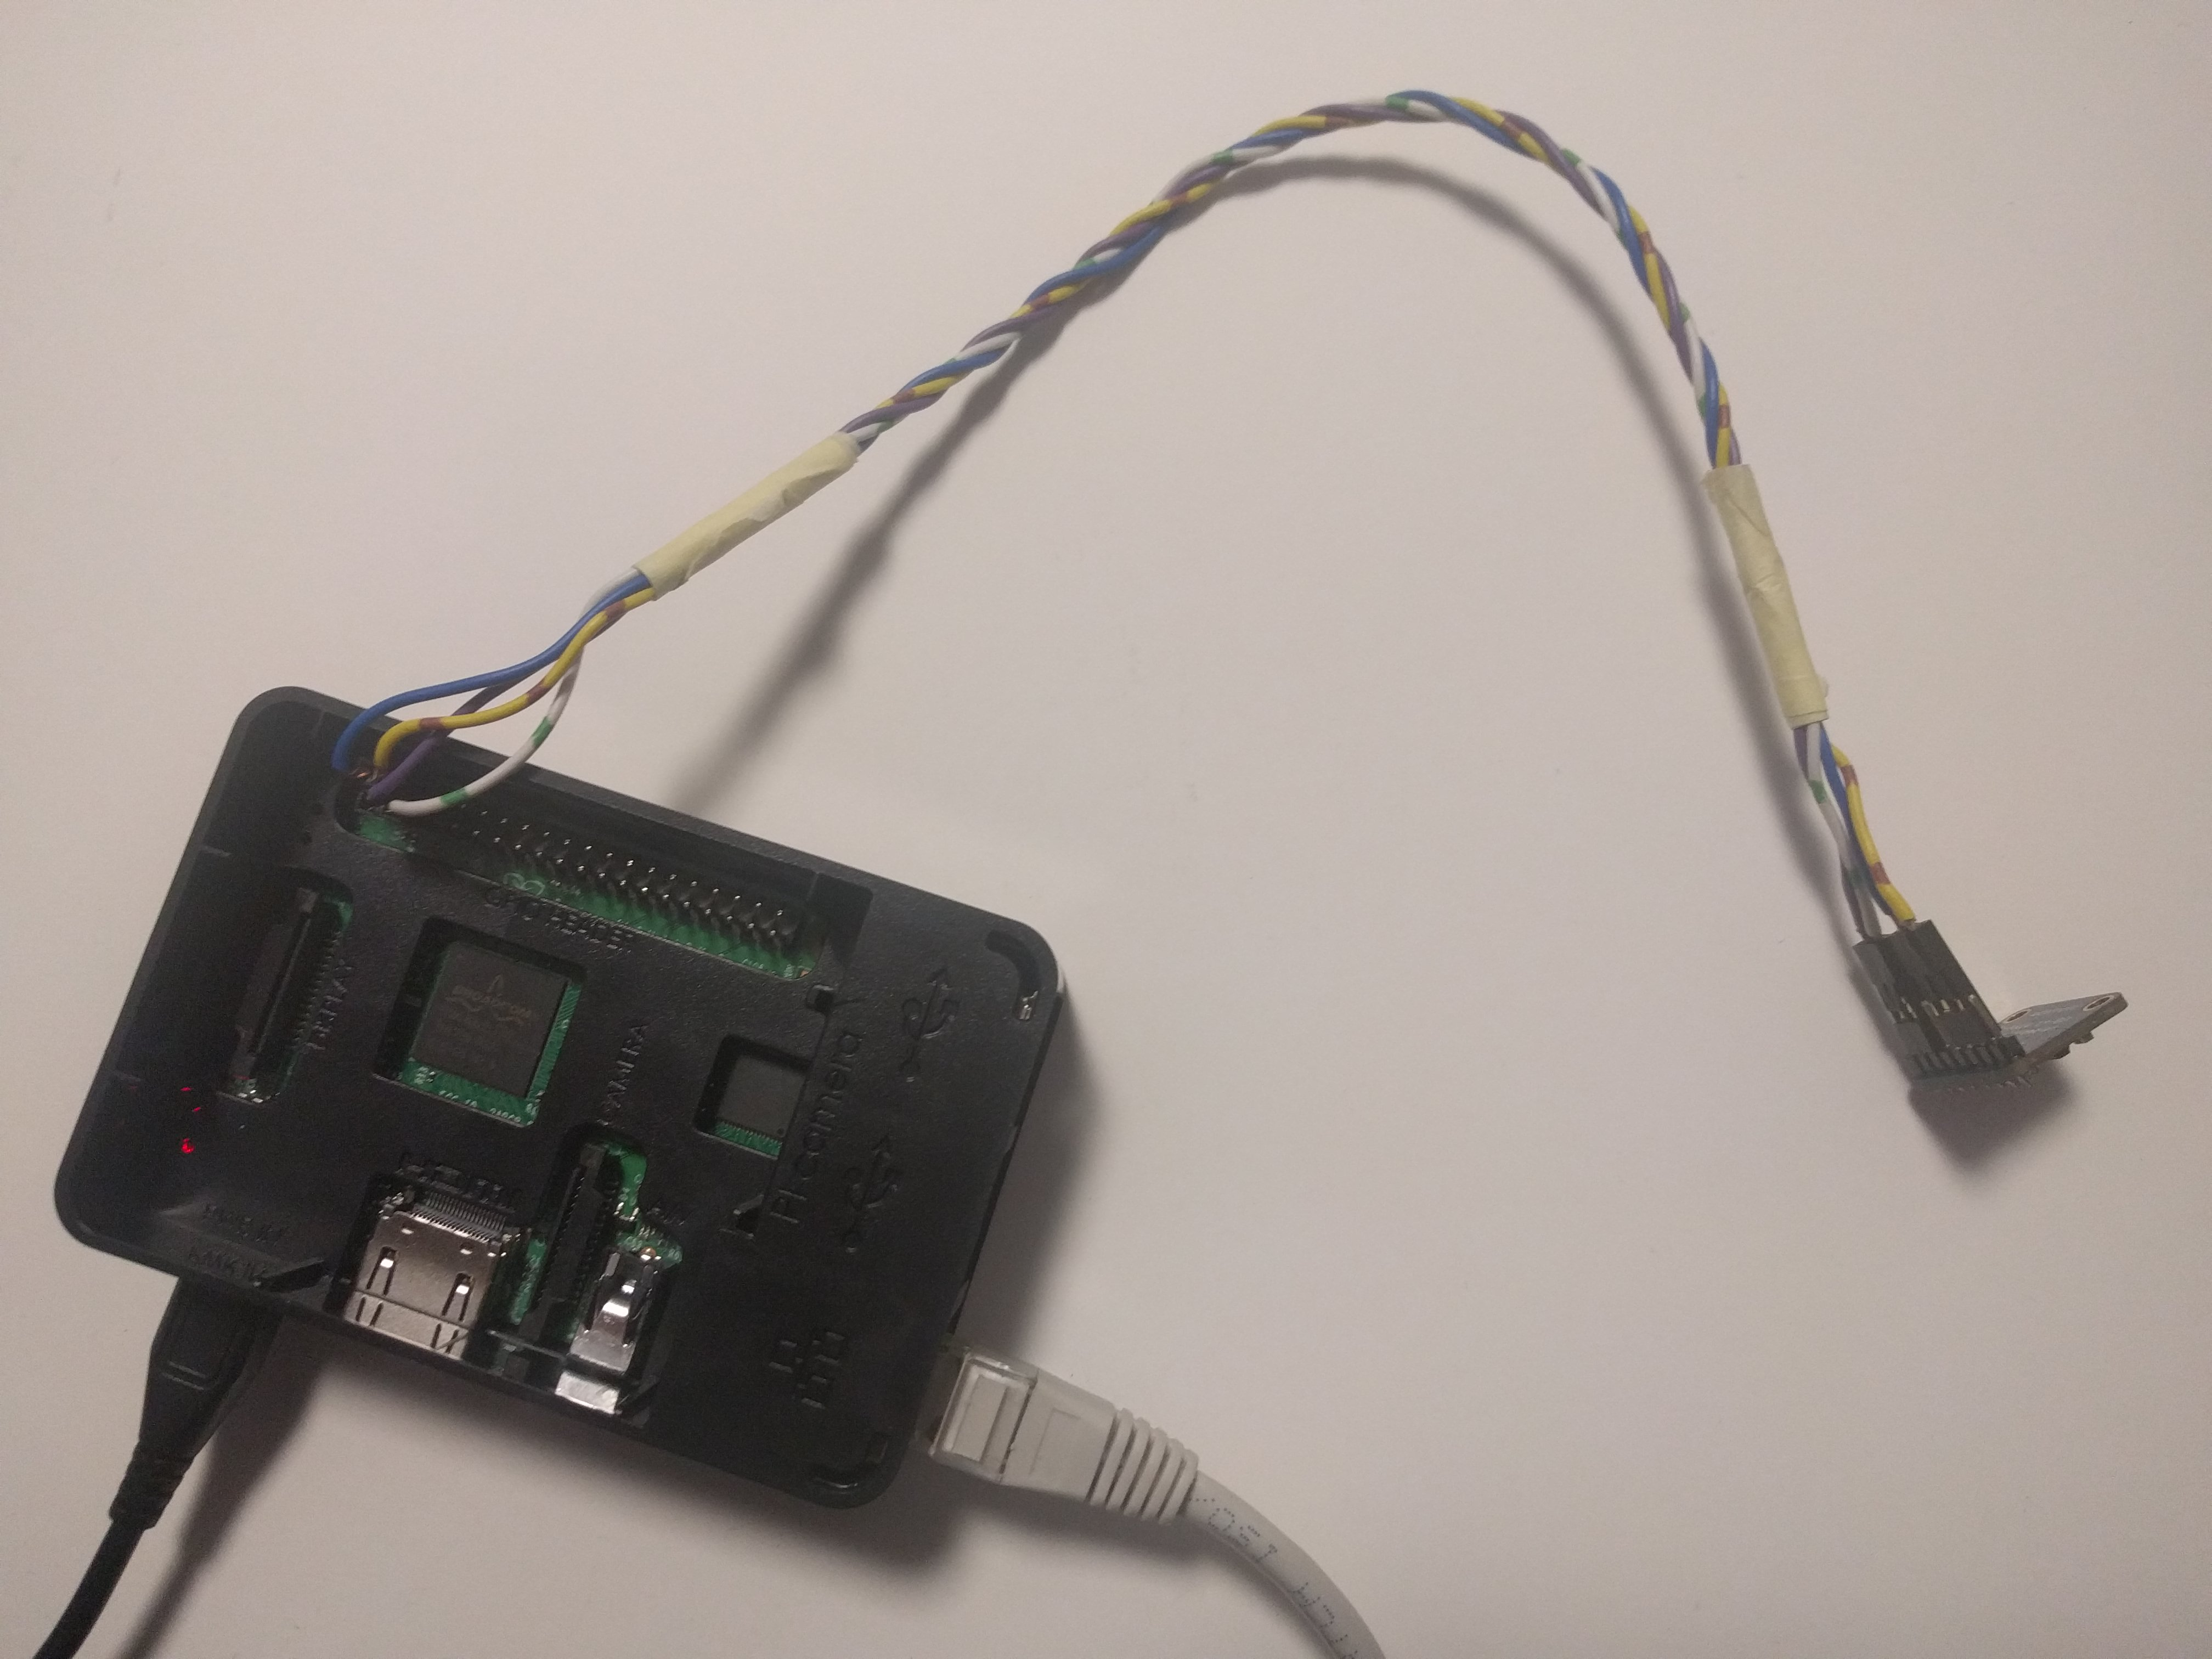
\includegraphics[width=\textwidth]{bitgraphics/pi.png}
  \caption{Wibroakustyczna stacja pomiarowa}
  \label{fig:foto}
\end{figure}

Od strony mikrokomputera Raspberry Pi obsługę wyżej wymienionych linii zapewnia
panel GPIO (General Purpose Input Output). Znajdują się w nim piny zasilające,
uziemienia, piny dedykowanych do konkretnych protokołów komunikacji, w tym
I\textsuperscript{2}C, i piny których przeznaczenie nie jest ustalone.  Na
poziomie oprogramowania do obsługi komunikacji przez wybrany protokół pomocny
jest pakiet narzędzi {\fontfamily{\ttdefault}\selectfont i2c-tools}, który
między innymi pozwala odczytać adres urządzeń podłączonych do magistrali.

Główną częścią projektu było napisanie biblioteki do obsługi używanego
akcelerometru, oraz kodu który ją wykorzystuje w celu nieprzerwanej akwizycji i
zapisu danych pomiarowych. Dokładne działanie urządzenia zostało opisane w
dokumentacji \cite{mma8451}. Komunikacja z urządzeniem, przez protokół
I\textsuperscript{2}C, polegała na zapisie i odczycie danych z rejestrów.
Pierwszym krokiem było stworzenie części biblioteki która w wygodny sposób
pozwoli ustawiać flagi (kombinacje bitów w rejestrach, które sygnalizują
urządzeniu pożądaną konfigurację) i odczytywać dane z tych rejestrów. W tym
celu stworzono klasy \lstinline|Flag| i \lstinline|Register|, które
przechowują liczby odpowiadające odpowiednio kombinacji bitów flagi i
adresowi rejestru (Kod źr. \ref{code:reg}).

\begin{program}
  \caption{Definicja rejestru \lstinline|STATUS| i jego flag}
  \begin{lstlisting}
    import mma8451.register.addr as REG
    from mma8451.register.classes import Flag

    class STATUS(Flag):
      _addr           = REG.STATUS
      ZYXOW           = 0x80
      ZOW             = 0x40
      YOW             = 0x20
      XOW             = 0x10
      ZYXDR           = 0x08
      ZDR             = 0x04
      YDR             = 0x02
      XDR             = 0x01
  \end{lstlisting}
  \label{code:reg}
\end{program}

Następnie stworzono klasę \lstinline|IIC|, która, posiada metody pozwalające na
zapis wartości do rejestrów, jak i odczyt wartości przy wykorzystaniu uprzednio
stworzonych typów. Szczególnie ważne było stworzenie metody pozyskiwania
wartości w trybie \emph{burst}, który pozwala na odczyt wielu wartości naraz
jednym ciągiem danych. Wykorzystuje ona bibliotekę \emph{pigpio}.

\begin{program}
  \caption{Wykorzystanie klasy IIC do poboru danych}
  \begin{lstlisting}
    from mma8451.register import register as REG
    from mma8451.iic import IIC
    import pigpio

    # Inicjalizacja połączenia z procesem pigpio
    pi = pigpio.pi()
    # Stwórz obiekt klasy, gdzie 1 do magistrala a 0x1D adres
    iic = IIC(pi, 1, 0x1D)
    # Uśpij urządzenie
    iic.unset_flag(REG.CTRL_REG1.ACTIVE)
    # Włącz tryb 14-to bitowy
    iic.unset_flag(REG.CTRL_REG1.F_READ)
    # Włacz urządzenie do trybu aktywnego
    iic.set_flag(REG.CTRL_REG1.ACTIVE)
    # Pobierz dane ze wszystkich trzech osi
    dane = iic.block_read(REG.OUT_X_MSB, 6)
  \end{lstlisting}
  \label{code:iic}
\end{program}

Po napisaniu tych elementów biblioteki zajęto się jej główną częścią, służącą
do inicjalizacji urządzenia, obsługi przerwań, ustawienia pożądanych parametrów
i przygotowania wątków i procesów ciągłej akwizycji i zapisu danych. W procesie
inicializacji ustawiane są flagi włączające tryb niskoszumowy urządzenia oraz
najmniej energooszczędny, natomiast najbardziej dokładny tryb próbkowania.
Ustawienia zakresu dynamicznego oraz częstotliwości próbkowania pozostawione są
na swoich domyślnych wartościach, odpowiednio $\pm\SI{2}{\g}$ oraz
\SI{800}{\hertz}. Pozwala to zapewnić maksymalną dokładność uzyskanych z
urządzenia danych.

Kolejno ustawiane są flagi które aktywują wbudowaną kolejkę FIFO (First In
First Out) urządzenia. Aby nie stracić żadnych próbek z powodu tymczasowego
spowolnienia wykonywania programu oraz by nie zajmować całego czasu procesora
poprzez ciągłe sprawdzanie rejestrów w oczekiwaniu na nowe próbki, jest
wykorzystana ta kolejka, która może przechowywać aż do trzydziestu dwóch
czternasto-bitowych próbek z trzech osi. Kolejka jest ustawiana tak, by w
momencie wykroczenia liczby próbek w kolejce ponad dwadzieścia następowało
przerwanie, wysyłane w postaci zmiany stanu na pinie \emph{I1} do GPIO.
W programie ustawiona jest by w momencie wykrycia tej zmiany została wykonana
funkcja, która informuje wątek akwizycji o dostępności nowych danych.

Po inicjalizacji ustawień uruchamiany jest wątek akwizycji danych oraz proces,
który się zajmuje ich zapisywaniem. Wątek akwizycji czeka na informację o
dostępności nowych danych po czym odczytuje wszystkie próbki z kolejki
wykorzystując do tego wspomniany wcześniej tryb \emph{burst}, a następnie
zebrane wartości przekazuje do kolejki. Na dane w kolejce czeka proces
zapisujący, który po zebraniu odpowiedniej ilości próbek, która w tym momencie
odpowiada pięciu minutom, przeprowadza zamianę uzyskanych wartości z kodu
uzupełnień do dwóch na liczbę całkowitą ze znakiem, po czym uzyskaną macierz
zawierającą dane ze wszystkich osi zapisuje do plik HDF5 w grupach
odpowiadających dacie i godzinie zapisu. Wybrano format HDF5 z powodu na jego
uniwersalność oraz wygodę wewnętrznej struktury (Rys. \ref{fig:struc}).

\begin{figure}[!tbh]%
  \centering%
  \begin{minipage}{0.3\textwidth}%
    \dirtree{%
      .1 <rok>/.
      .2 <miesiąc>/.
      .3 <dzień>/.
      .4 <godzina>/.
      .5 <minuta>.
      .5 \dots.
      .4 \dots.
      .3 \dots.
      .2 \dots.
    }%
  \end{minipage}%
  \caption{Struktura grup w pliku z danymi}%
  \label{fig:struc}%
\end{figure}%

% opis kodu

Stacja pomiarowa jest zdolna do zapisania w swojej pamięci wewnętrznej około
miesiąca wibrogramu. Ponieważ norma wymaga analizy tercjowej drgań, uwzględniono
filtrację sygnału w pasmach od \SI{0,5}{\hertz} do \SI{100}{\hertz}.

\begin{figure}[!tbh]
  \centering
  \includegraphics[width=0.8\textwidth, angle=-90]{bitgraphics/pom_2.jpg}
  \caption{Stacja pomiarowa podczas pracy}
  \label{fig:pomiar1}
\end{figure}

\begin{figure}[!tbh]
  \centering
  \includegraphics[width=0.8\textwidth]{bitgraphics/pom_1.jpg}
  \caption{Tymczasowe mocowanie akcelerometru}
  \label{fig:imadlo}
\end{figure}

\begin{figure}[!tbh]
  \centering
  %% Creator: Matplotlib, PGF backend
%%
%% To include the figure in your LaTeX document, write
%%   \input{<filename>.pgf}
%%
%% Make sure the required packages are loaded in your preamble
%%   \usepackage{pgf}
%%
%% Figures using additional raster images can only be included by \input if
%% they are in the same directory as the main LaTeX file. For loading figures
%% from other directories you can use the `import` package
%%   \usepackage{import}
%% and then include the figures with
%%   \import{<path to file>}{<filename>.pgf}
%%
%% Matplotlib used the following preamble
%%   \usepackage[utf8]{inputenc}
%%   \usepackage[T1]{fontenc}
%%   \usepackage{siunitx}
%%
\begingroup%
\makeatletter%
\begin{pgfpicture}%
\pgfpathrectangle{\pgfpointorigin}{\pgfqpoint{5.000000in}{3.500000in}}%
\pgfusepath{use as bounding box, clip}%
\begin{pgfscope}%
\pgfsetbuttcap%
\pgfsetmiterjoin%
\definecolor{currentfill}{rgb}{1.000000,1.000000,1.000000}%
\pgfsetfillcolor{currentfill}%
\pgfsetlinewidth{0.000000pt}%
\definecolor{currentstroke}{rgb}{1.000000,1.000000,1.000000}%
\pgfsetstrokecolor{currentstroke}%
\pgfsetdash{}{0pt}%
\pgfpathmoveto{\pgfqpoint{0.000000in}{0.000000in}}%
\pgfpathlineto{\pgfqpoint{5.000000in}{0.000000in}}%
\pgfpathlineto{\pgfqpoint{5.000000in}{3.500000in}}%
\pgfpathlineto{\pgfqpoint{0.000000in}{3.500000in}}%
\pgfpathclose%
\pgfusepath{fill}%
\end{pgfscope}%
\begin{pgfscope}%
\pgfsetbuttcap%
\pgfsetmiterjoin%
\definecolor{currentfill}{rgb}{1.000000,1.000000,1.000000}%
\pgfsetfillcolor{currentfill}%
\pgfsetlinewidth{0.000000pt}%
\definecolor{currentstroke}{rgb}{0.000000,0.000000,0.000000}%
\pgfsetstrokecolor{currentstroke}%
\pgfsetstrokeopacity{0.000000}%
\pgfsetdash{}{0pt}%
\pgfpathmoveto{\pgfqpoint{0.967524in}{0.564288in}}%
\pgfpathlineto{\pgfqpoint{4.815000in}{0.564288in}}%
\pgfpathlineto{\pgfqpoint{4.815000in}{3.315000in}}%
\pgfpathlineto{\pgfqpoint{0.967524in}{3.315000in}}%
\pgfpathclose%
\pgfusepath{fill}%
\end{pgfscope}%
\begin{pgfscope}%
\pgfpathrectangle{\pgfqpoint{0.967524in}{0.564288in}}{\pgfqpoint{3.847476in}{2.750712in}}%
\pgfusepath{clip}%
\pgfsetrectcap%
\pgfsetroundjoin%
\pgfsetlinewidth{0.803000pt}%
\definecolor{currentstroke}{rgb}{0.690196,0.690196,0.690196}%
\pgfsetstrokecolor{currentstroke}%
\pgfsetdash{}{0pt}%
\pgfpathmoveto{\pgfqpoint{1.142409in}{0.564288in}}%
\pgfpathlineto{\pgfqpoint{1.142409in}{3.315000in}}%
\pgfusepath{stroke}%
\end{pgfscope}%
\begin{pgfscope}%
\pgfsetbuttcap%
\pgfsetroundjoin%
\definecolor{currentfill}{rgb}{0.000000,0.000000,0.000000}%
\pgfsetfillcolor{currentfill}%
\pgfsetlinewidth{0.803000pt}%
\definecolor{currentstroke}{rgb}{0.000000,0.000000,0.000000}%
\pgfsetstrokecolor{currentstroke}%
\pgfsetdash{}{0pt}%
\pgfsys@defobject{currentmarker}{\pgfqpoint{0.000000in}{-0.048611in}}{\pgfqpoint{0.000000in}{0.000000in}}{%
\pgfpathmoveto{\pgfqpoint{0.000000in}{0.000000in}}%
\pgfpathlineto{\pgfqpoint{0.000000in}{-0.048611in}}%
\pgfusepath{stroke,fill}%
}%
\begin{pgfscope}%
\pgfsys@transformshift{1.142409in}{0.564288in}%
\pgfsys@useobject{currentmarker}{}%
\end{pgfscope}%
\end{pgfscope}%
\begin{pgfscope}%
\pgftext[x=1.142409in,y=0.467066in,,top]{\rmfamily\fontsize{10.000000}{12.000000}\selectfont \(\displaystyle 0,0\)}%
\end{pgfscope}%
\begin{pgfscope}%
\pgfpathrectangle{\pgfqpoint{0.967524in}{0.564288in}}{\pgfqpoint{3.847476in}{2.750712in}}%
\pgfusepath{clip}%
\pgfsetrectcap%
\pgfsetroundjoin%
\pgfsetlinewidth{0.803000pt}%
\definecolor{currentstroke}{rgb}{0.690196,0.690196,0.690196}%
\pgfsetstrokecolor{currentstroke}%
\pgfsetdash{}{0pt}%
\pgfpathmoveto{\pgfqpoint{1.702602in}{0.564288in}}%
\pgfpathlineto{\pgfqpoint{1.702602in}{3.315000in}}%
\pgfusepath{stroke}%
\end{pgfscope}%
\begin{pgfscope}%
\pgfsetbuttcap%
\pgfsetroundjoin%
\definecolor{currentfill}{rgb}{0.000000,0.000000,0.000000}%
\pgfsetfillcolor{currentfill}%
\pgfsetlinewidth{0.803000pt}%
\definecolor{currentstroke}{rgb}{0.000000,0.000000,0.000000}%
\pgfsetstrokecolor{currentstroke}%
\pgfsetdash{}{0pt}%
\pgfsys@defobject{currentmarker}{\pgfqpoint{0.000000in}{-0.048611in}}{\pgfqpoint{0.000000in}{0.000000in}}{%
\pgfpathmoveto{\pgfqpoint{0.000000in}{0.000000in}}%
\pgfpathlineto{\pgfqpoint{0.000000in}{-0.048611in}}%
\pgfusepath{stroke,fill}%
}%
\begin{pgfscope}%
\pgfsys@transformshift{1.702602in}{0.564288in}%
\pgfsys@useobject{currentmarker}{}%
\end{pgfscope}%
\end{pgfscope}%
\begin{pgfscope}%
\pgftext[x=1.702602in,y=0.467066in,,top]{\rmfamily\fontsize{10.000000}{12.000000}\selectfont \(\displaystyle 0,2\)}%
\end{pgfscope}%
\begin{pgfscope}%
\pgfpathrectangle{\pgfqpoint{0.967524in}{0.564288in}}{\pgfqpoint{3.847476in}{2.750712in}}%
\pgfusepath{clip}%
\pgfsetrectcap%
\pgfsetroundjoin%
\pgfsetlinewidth{0.803000pt}%
\definecolor{currentstroke}{rgb}{0.690196,0.690196,0.690196}%
\pgfsetstrokecolor{currentstroke}%
\pgfsetdash{}{0pt}%
\pgfpathmoveto{\pgfqpoint{2.262795in}{0.564288in}}%
\pgfpathlineto{\pgfqpoint{2.262795in}{3.315000in}}%
\pgfusepath{stroke}%
\end{pgfscope}%
\begin{pgfscope}%
\pgfsetbuttcap%
\pgfsetroundjoin%
\definecolor{currentfill}{rgb}{0.000000,0.000000,0.000000}%
\pgfsetfillcolor{currentfill}%
\pgfsetlinewidth{0.803000pt}%
\definecolor{currentstroke}{rgb}{0.000000,0.000000,0.000000}%
\pgfsetstrokecolor{currentstroke}%
\pgfsetdash{}{0pt}%
\pgfsys@defobject{currentmarker}{\pgfqpoint{0.000000in}{-0.048611in}}{\pgfqpoint{0.000000in}{0.000000in}}{%
\pgfpathmoveto{\pgfqpoint{0.000000in}{0.000000in}}%
\pgfpathlineto{\pgfqpoint{0.000000in}{-0.048611in}}%
\pgfusepath{stroke,fill}%
}%
\begin{pgfscope}%
\pgfsys@transformshift{2.262795in}{0.564288in}%
\pgfsys@useobject{currentmarker}{}%
\end{pgfscope}%
\end{pgfscope}%
\begin{pgfscope}%
\pgftext[x=2.262795in,y=0.467066in,,top]{\rmfamily\fontsize{10.000000}{12.000000}\selectfont \(\displaystyle 0,4\)}%
\end{pgfscope}%
\begin{pgfscope}%
\pgfpathrectangle{\pgfqpoint{0.967524in}{0.564288in}}{\pgfqpoint{3.847476in}{2.750712in}}%
\pgfusepath{clip}%
\pgfsetrectcap%
\pgfsetroundjoin%
\pgfsetlinewidth{0.803000pt}%
\definecolor{currentstroke}{rgb}{0.690196,0.690196,0.690196}%
\pgfsetstrokecolor{currentstroke}%
\pgfsetdash{}{0pt}%
\pgfpathmoveto{\pgfqpoint{2.822988in}{0.564288in}}%
\pgfpathlineto{\pgfqpoint{2.822988in}{3.315000in}}%
\pgfusepath{stroke}%
\end{pgfscope}%
\begin{pgfscope}%
\pgfsetbuttcap%
\pgfsetroundjoin%
\definecolor{currentfill}{rgb}{0.000000,0.000000,0.000000}%
\pgfsetfillcolor{currentfill}%
\pgfsetlinewidth{0.803000pt}%
\definecolor{currentstroke}{rgb}{0.000000,0.000000,0.000000}%
\pgfsetstrokecolor{currentstroke}%
\pgfsetdash{}{0pt}%
\pgfsys@defobject{currentmarker}{\pgfqpoint{0.000000in}{-0.048611in}}{\pgfqpoint{0.000000in}{0.000000in}}{%
\pgfpathmoveto{\pgfqpoint{0.000000in}{0.000000in}}%
\pgfpathlineto{\pgfqpoint{0.000000in}{-0.048611in}}%
\pgfusepath{stroke,fill}%
}%
\begin{pgfscope}%
\pgfsys@transformshift{2.822988in}{0.564288in}%
\pgfsys@useobject{currentmarker}{}%
\end{pgfscope}%
\end{pgfscope}%
\begin{pgfscope}%
\pgftext[x=2.822988in,y=0.467066in,,top]{\rmfamily\fontsize{10.000000}{12.000000}\selectfont \(\displaystyle 0,6\)}%
\end{pgfscope}%
\begin{pgfscope}%
\pgfpathrectangle{\pgfqpoint{0.967524in}{0.564288in}}{\pgfqpoint{3.847476in}{2.750712in}}%
\pgfusepath{clip}%
\pgfsetrectcap%
\pgfsetroundjoin%
\pgfsetlinewidth{0.803000pt}%
\definecolor{currentstroke}{rgb}{0.690196,0.690196,0.690196}%
\pgfsetstrokecolor{currentstroke}%
\pgfsetdash{}{0pt}%
\pgfpathmoveto{\pgfqpoint{3.383181in}{0.564288in}}%
\pgfpathlineto{\pgfqpoint{3.383181in}{3.315000in}}%
\pgfusepath{stroke}%
\end{pgfscope}%
\begin{pgfscope}%
\pgfsetbuttcap%
\pgfsetroundjoin%
\definecolor{currentfill}{rgb}{0.000000,0.000000,0.000000}%
\pgfsetfillcolor{currentfill}%
\pgfsetlinewidth{0.803000pt}%
\definecolor{currentstroke}{rgb}{0.000000,0.000000,0.000000}%
\pgfsetstrokecolor{currentstroke}%
\pgfsetdash{}{0pt}%
\pgfsys@defobject{currentmarker}{\pgfqpoint{0.000000in}{-0.048611in}}{\pgfqpoint{0.000000in}{0.000000in}}{%
\pgfpathmoveto{\pgfqpoint{0.000000in}{0.000000in}}%
\pgfpathlineto{\pgfqpoint{0.000000in}{-0.048611in}}%
\pgfusepath{stroke,fill}%
}%
\begin{pgfscope}%
\pgfsys@transformshift{3.383181in}{0.564288in}%
\pgfsys@useobject{currentmarker}{}%
\end{pgfscope}%
\end{pgfscope}%
\begin{pgfscope}%
\pgftext[x=3.383181in,y=0.467066in,,top]{\rmfamily\fontsize{10.000000}{12.000000}\selectfont \(\displaystyle 0,8\)}%
\end{pgfscope}%
\begin{pgfscope}%
\pgfpathrectangle{\pgfqpoint{0.967524in}{0.564288in}}{\pgfqpoint{3.847476in}{2.750712in}}%
\pgfusepath{clip}%
\pgfsetrectcap%
\pgfsetroundjoin%
\pgfsetlinewidth{0.803000pt}%
\definecolor{currentstroke}{rgb}{0.690196,0.690196,0.690196}%
\pgfsetstrokecolor{currentstroke}%
\pgfsetdash{}{0pt}%
\pgfpathmoveto{\pgfqpoint{3.943375in}{0.564288in}}%
\pgfpathlineto{\pgfqpoint{3.943375in}{3.315000in}}%
\pgfusepath{stroke}%
\end{pgfscope}%
\begin{pgfscope}%
\pgfsetbuttcap%
\pgfsetroundjoin%
\definecolor{currentfill}{rgb}{0.000000,0.000000,0.000000}%
\pgfsetfillcolor{currentfill}%
\pgfsetlinewidth{0.803000pt}%
\definecolor{currentstroke}{rgb}{0.000000,0.000000,0.000000}%
\pgfsetstrokecolor{currentstroke}%
\pgfsetdash{}{0pt}%
\pgfsys@defobject{currentmarker}{\pgfqpoint{0.000000in}{-0.048611in}}{\pgfqpoint{0.000000in}{0.000000in}}{%
\pgfpathmoveto{\pgfqpoint{0.000000in}{0.000000in}}%
\pgfpathlineto{\pgfqpoint{0.000000in}{-0.048611in}}%
\pgfusepath{stroke,fill}%
}%
\begin{pgfscope}%
\pgfsys@transformshift{3.943375in}{0.564288in}%
\pgfsys@useobject{currentmarker}{}%
\end{pgfscope}%
\end{pgfscope}%
\begin{pgfscope}%
\pgftext[x=3.943375in,y=0.467066in,,top]{\rmfamily\fontsize{10.000000}{12.000000}\selectfont \(\displaystyle 1,0\)}%
\end{pgfscope}%
\begin{pgfscope}%
\pgfpathrectangle{\pgfqpoint{0.967524in}{0.564288in}}{\pgfqpoint{3.847476in}{2.750712in}}%
\pgfusepath{clip}%
\pgfsetrectcap%
\pgfsetroundjoin%
\pgfsetlinewidth{0.803000pt}%
\definecolor{currentstroke}{rgb}{0.690196,0.690196,0.690196}%
\pgfsetstrokecolor{currentstroke}%
\pgfsetdash{}{0pt}%
\pgfpathmoveto{\pgfqpoint{4.503568in}{0.564288in}}%
\pgfpathlineto{\pgfqpoint{4.503568in}{3.315000in}}%
\pgfusepath{stroke}%
\end{pgfscope}%
\begin{pgfscope}%
\pgfsetbuttcap%
\pgfsetroundjoin%
\definecolor{currentfill}{rgb}{0.000000,0.000000,0.000000}%
\pgfsetfillcolor{currentfill}%
\pgfsetlinewidth{0.803000pt}%
\definecolor{currentstroke}{rgb}{0.000000,0.000000,0.000000}%
\pgfsetstrokecolor{currentstroke}%
\pgfsetdash{}{0pt}%
\pgfsys@defobject{currentmarker}{\pgfqpoint{0.000000in}{-0.048611in}}{\pgfqpoint{0.000000in}{0.000000in}}{%
\pgfpathmoveto{\pgfqpoint{0.000000in}{0.000000in}}%
\pgfpathlineto{\pgfqpoint{0.000000in}{-0.048611in}}%
\pgfusepath{stroke,fill}%
}%
\begin{pgfscope}%
\pgfsys@transformshift{4.503568in}{0.564288in}%
\pgfsys@useobject{currentmarker}{}%
\end{pgfscope}%
\end{pgfscope}%
\begin{pgfscope}%
\pgftext[x=4.503568in,y=0.467066in,,top]{\rmfamily\fontsize{10.000000}{12.000000}\selectfont \(\displaystyle 1,2\)}%
\end{pgfscope}%
\begin{pgfscope}%
\pgftext[x=2.891262in,y=0.288855in,,top]{\rmfamily\fontsize{10.000000}{12.000000}\selectfont Czas [\si{\second}]}%
\end{pgfscope}%
\begin{pgfscope}%
\pgfpathrectangle{\pgfqpoint{0.967524in}{0.564288in}}{\pgfqpoint{3.847476in}{2.750712in}}%
\pgfusepath{clip}%
\pgfsetrectcap%
\pgfsetroundjoin%
\pgfsetlinewidth{0.803000pt}%
\definecolor{currentstroke}{rgb}{0.690196,0.690196,0.690196}%
\pgfsetstrokecolor{currentstroke}%
\pgfsetdash{}{0pt}%
\pgfpathmoveto{\pgfqpoint{0.967524in}{0.932258in}}%
\pgfpathlineto{\pgfqpoint{4.815000in}{0.932258in}}%
\pgfusepath{stroke}%
\end{pgfscope}%
\begin{pgfscope}%
\pgfsetbuttcap%
\pgfsetroundjoin%
\definecolor{currentfill}{rgb}{0.000000,0.000000,0.000000}%
\pgfsetfillcolor{currentfill}%
\pgfsetlinewidth{0.803000pt}%
\definecolor{currentstroke}{rgb}{0.000000,0.000000,0.000000}%
\pgfsetstrokecolor{currentstroke}%
\pgfsetdash{}{0pt}%
\pgfsys@defobject{currentmarker}{\pgfqpoint{-0.048611in}{0.000000in}}{\pgfqpoint{0.000000in}{0.000000in}}{%
\pgfpathmoveto{\pgfqpoint{0.000000in}{0.000000in}}%
\pgfpathlineto{\pgfqpoint{-0.048611in}{0.000000in}}%
\pgfusepath{stroke,fill}%
}%
\begin{pgfscope}%
\pgfsys@transformshift{0.967524in}{0.932258in}%
\pgfsys@useobject{currentmarker}{}%
\end{pgfscope}%
\end{pgfscope}%
\begin{pgfscope}%
\pgftext[x=0.353325in,y=0.884434in,left,base]{\rmfamily\fontsize{10.000000}{12.000000}\selectfont \(\displaystyle -10,025\)}%
\end{pgfscope}%
\begin{pgfscope}%
\pgfpathrectangle{\pgfqpoint{0.967524in}{0.564288in}}{\pgfqpoint{3.847476in}{2.750712in}}%
\pgfusepath{clip}%
\pgfsetrectcap%
\pgfsetroundjoin%
\pgfsetlinewidth{0.803000pt}%
\definecolor{currentstroke}{rgb}{0.690196,0.690196,0.690196}%
\pgfsetstrokecolor{currentstroke}%
\pgfsetdash{}{0pt}%
\pgfpathmoveto{\pgfqpoint{0.967524in}{1.305279in}}%
\pgfpathlineto{\pgfqpoint{4.815000in}{1.305279in}}%
\pgfusepath{stroke}%
\end{pgfscope}%
\begin{pgfscope}%
\pgfsetbuttcap%
\pgfsetroundjoin%
\definecolor{currentfill}{rgb}{0.000000,0.000000,0.000000}%
\pgfsetfillcolor{currentfill}%
\pgfsetlinewidth{0.803000pt}%
\definecolor{currentstroke}{rgb}{0.000000,0.000000,0.000000}%
\pgfsetstrokecolor{currentstroke}%
\pgfsetdash{}{0pt}%
\pgfsys@defobject{currentmarker}{\pgfqpoint{-0.048611in}{0.000000in}}{\pgfqpoint{0.000000in}{0.000000in}}{%
\pgfpathmoveto{\pgfqpoint{0.000000in}{0.000000in}}%
\pgfpathlineto{\pgfqpoint{-0.048611in}{0.000000in}}%
\pgfusepath{stroke,fill}%
}%
\begin{pgfscope}%
\pgfsys@transformshift{0.967524in}{1.305279in}%
\pgfsys@useobject{currentmarker}{}%
\end{pgfscope}%
\end{pgfscope}%
\begin{pgfscope}%
\pgftext[x=0.353325in,y=1.257455in,left,base]{\rmfamily\fontsize{10.000000}{12.000000}\selectfont \(\displaystyle -10,000\)}%
\end{pgfscope}%
\begin{pgfscope}%
\pgfpathrectangle{\pgfqpoint{0.967524in}{0.564288in}}{\pgfqpoint{3.847476in}{2.750712in}}%
\pgfusepath{clip}%
\pgfsetrectcap%
\pgfsetroundjoin%
\pgfsetlinewidth{0.803000pt}%
\definecolor{currentstroke}{rgb}{0.690196,0.690196,0.690196}%
\pgfsetstrokecolor{currentstroke}%
\pgfsetdash{}{0pt}%
\pgfpathmoveto{\pgfqpoint{0.967524in}{1.678301in}}%
\pgfpathlineto{\pgfqpoint{4.815000in}{1.678301in}}%
\pgfusepath{stroke}%
\end{pgfscope}%
\begin{pgfscope}%
\pgfsetbuttcap%
\pgfsetroundjoin%
\definecolor{currentfill}{rgb}{0.000000,0.000000,0.000000}%
\pgfsetfillcolor{currentfill}%
\pgfsetlinewidth{0.803000pt}%
\definecolor{currentstroke}{rgb}{0.000000,0.000000,0.000000}%
\pgfsetstrokecolor{currentstroke}%
\pgfsetdash{}{0pt}%
\pgfsys@defobject{currentmarker}{\pgfqpoint{-0.048611in}{0.000000in}}{\pgfqpoint{0.000000in}{0.000000in}}{%
\pgfpathmoveto{\pgfqpoint{0.000000in}{0.000000in}}%
\pgfpathlineto{\pgfqpoint{-0.048611in}{0.000000in}}%
\pgfusepath{stroke,fill}%
}%
\begin{pgfscope}%
\pgfsys@transformshift{0.967524in}{1.678301in}%
\pgfsys@useobject{currentmarker}{}%
\end{pgfscope}%
\end{pgfscope}%
\begin{pgfscope}%
\pgftext[x=0.422770in,y=1.630476in,left,base]{\rmfamily\fontsize{10.000000}{12.000000}\selectfont \(\displaystyle -9,975\)}%
\end{pgfscope}%
\begin{pgfscope}%
\pgfpathrectangle{\pgfqpoint{0.967524in}{0.564288in}}{\pgfqpoint{3.847476in}{2.750712in}}%
\pgfusepath{clip}%
\pgfsetrectcap%
\pgfsetroundjoin%
\pgfsetlinewidth{0.803000pt}%
\definecolor{currentstroke}{rgb}{0.690196,0.690196,0.690196}%
\pgfsetstrokecolor{currentstroke}%
\pgfsetdash{}{0pt}%
\pgfpathmoveto{\pgfqpoint{0.967524in}{2.051322in}}%
\pgfpathlineto{\pgfqpoint{4.815000in}{2.051322in}}%
\pgfusepath{stroke}%
\end{pgfscope}%
\begin{pgfscope}%
\pgfsetbuttcap%
\pgfsetroundjoin%
\definecolor{currentfill}{rgb}{0.000000,0.000000,0.000000}%
\pgfsetfillcolor{currentfill}%
\pgfsetlinewidth{0.803000pt}%
\definecolor{currentstroke}{rgb}{0.000000,0.000000,0.000000}%
\pgfsetstrokecolor{currentstroke}%
\pgfsetdash{}{0pt}%
\pgfsys@defobject{currentmarker}{\pgfqpoint{-0.048611in}{0.000000in}}{\pgfqpoint{0.000000in}{0.000000in}}{%
\pgfpathmoveto{\pgfqpoint{0.000000in}{0.000000in}}%
\pgfpathlineto{\pgfqpoint{-0.048611in}{0.000000in}}%
\pgfusepath{stroke,fill}%
}%
\begin{pgfscope}%
\pgfsys@transformshift{0.967524in}{2.051322in}%
\pgfsys@useobject{currentmarker}{}%
\end{pgfscope}%
\end{pgfscope}%
\begin{pgfscope}%
\pgftext[x=0.422770in,y=2.003498in,left,base]{\rmfamily\fontsize{10.000000}{12.000000}\selectfont \(\displaystyle -9,950\)}%
\end{pgfscope}%
\begin{pgfscope}%
\pgfpathrectangle{\pgfqpoint{0.967524in}{0.564288in}}{\pgfqpoint{3.847476in}{2.750712in}}%
\pgfusepath{clip}%
\pgfsetrectcap%
\pgfsetroundjoin%
\pgfsetlinewidth{0.803000pt}%
\definecolor{currentstroke}{rgb}{0.690196,0.690196,0.690196}%
\pgfsetstrokecolor{currentstroke}%
\pgfsetdash{}{0pt}%
\pgfpathmoveto{\pgfqpoint{0.967524in}{2.424343in}}%
\pgfpathlineto{\pgfqpoint{4.815000in}{2.424343in}}%
\pgfusepath{stroke}%
\end{pgfscope}%
\begin{pgfscope}%
\pgfsetbuttcap%
\pgfsetroundjoin%
\definecolor{currentfill}{rgb}{0.000000,0.000000,0.000000}%
\pgfsetfillcolor{currentfill}%
\pgfsetlinewidth{0.803000pt}%
\definecolor{currentstroke}{rgb}{0.000000,0.000000,0.000000}%
\pgfsetstrokecolor{currentstroke}%
\pgfsetdash{}{0pt}%
\pgfsys@defobject{currentmarker}{\pgfqpoint{-0.048611in}{0.000000in}}{\pgfqpoint{0.000000in}{0.000000in}}{%
\pgfpathmoveto{\pgfqpoint{0.000000in}{0.000000in}}%
\pgfpathlineto{\pgfqpoint{-0.048611in}{0.000000in}}%
\pgfusepath{stroke,fill}%
}%
\begin{pgfscope}%
\pgfsys@transformshift{0.967524in}{2.424343in}%
\pgfsys@useobject{currentmarker}{}%
\end{pgfscope}%
\end{pgfscope}%
\begin{pgfscope}%
\pgftext[x=0.422770in,y=2.376519in,left,base]{\rmfamily\fontsize{10.000000}{12.000000}\selectfont \(\displaystyle -9,925\)}%
\end{pgfscope}%
\begin{pgfscope}%
\pgfpathrectangle{\pgfqpoint{0.967524in}{0.564288in}}{\pgfqpoint{3.847476in}{2.750712in}}%
\pgfusepath{clip}%
\pgfsetrectcap%
\pgfsetroundjoin%
\pgfsetlinewidth{0.803000pt}%
\definecolor{currentstroke}{rgb}{0.690196,0.690196,0.690196}%
\pgfsetstrokecolor{currentstroke}%
\pgfsetdash{}{0pt}%
\pgfpathmoveto{\pgfqpoint{0.967524in}{2.797365in}}%
\pgfpathlineto{\pgfqpoint{4.815000in}{2.797365in}}%
\pgfusepath{stroke}%
\end{pgfscope}%
\begin{pgfscope}%
\pgfsetbuttcap%
\pgfsetroundjoin%
\definecolor{currentfill}{rgb}{0.000000,0.000000,0.000000}%
\pgfsetfillcolor{currentfill}%
\pgfsetlinewidth{0.803000pt}%
\definecolor{currentstroke}{rgb}{0.000000,0.000000,0.000000}%
\pgfsetstrokecolor{currentstroke}%
\pgfsetdash{}{0pt}%
\pgfsys@defobject{currentmarker}{\pgfqpoint{-0.048611in}{0.000000in}}{\pgfqpoint{0.000000in}{0.000000in}}{%
\pgfpathmoveto{\pgfqpoint{0.000000in}{0.000000in}}%
\pgfpathlineto{\pgfqpoint{-0.048611in}{0.000000in}}%
\pgfusepath{stroke,fill}%
}%
\begin{pgfscope}%
\pgfsys@transformshift{0.967524in}{2.797365in}%
\pgfsys@useobject{currentmarker}{}%
\end{pgfscope}%
\end{pgfscope}%
\begin{pgfscope}%
\pgftext[x=0.422770in,y=2.749540in,left,base]{\rmfamily\fontsize{10.000000}{12.000000}\selectfont \(\displaystyle -9,900\)}%
\end{pgfscope}%
\begin{pgfscope}%
\pgfpathrectangle{\pgfqpoint{0.967524in}{0.564288in}}{\pgfqpoint{3.847476in}{2.750712in}}%
\pgfusepath{clip}%
\pgfsetrectcap%
\pgfsetroundjoin%
\pgfsetlinewidth{0.803000pt}%
\definecolor{currentstroke}{rgb}{0.690196,0.690196,0.690196}%
\pgfsetstrokecolor{currentstroke}%
\pgfsetdash{}{0pt}%
\pgfpathmoveto{\pgfqpoint{0.967524in}{3.170386in}}%
\pgfpathlineto{\pgfqpoint{4.815000in}{3.170386in}}%
\pgfusepath{stroke}%
\end{pgfscope}%
\begin{pgfscope}%
\pgfsetbuttcap%
\pgfsetroundjoin%
\definecolor{currentfill}{rgb}{0.000000,0.000000,0.000000}%
\pgfsetfillcolor{currentfill}%
\pgfsetlinewidth{0.803000pt}%
\definecolor{currentstroke}{rgb}{0.000000,0.000000,0.000000}%
\pgfsetstrokecolor{currentstroke}%
\pgfsetdash{}{0pt}%
\pgfsys@defobject{currentmarker}{\pgfqpoint{-0.048611in}{0.000000in}}{\pgfqpoint{0.000000in}{0.000000in}}{%
\pgfpathmoveto{\pgfqpoint{0.000000in}{0.000000in}}%
\pgfpathlineto{\pgfqpoint{-0.048611in}{0.000000in}}%
\pgfusepath{stroke,fill}%
}%
\begin{pgfscope}%
\pgfsys@transformshift{0.967524in}{3.170386in}%
\pgfsys@useobject{currentmarker}{}%
\end{pgfscope}%
\end{pgfscope}%
\begin{pgfscope}%
\pgftext[x=0.422770in,y=3.122562in,left,base]{\rmfamily\fontsize{10.000000}{12.000000}\selectfont \(\displaystyle -9,875\)}%
\end{pgfscope}%
\begin{pgfscope}%
\pgftext[x=0.297770in,y=1.939644in,,bottom,rotate=90.000000]{\rmfamily\fontsize{10.000000}{12.000000}\selectfont Przyspieszenie drgań [\si{\meter\per\second\squared}]}%
\end{pgfscope}%
\begin{pgfscope}%
\pgfpathrectangle{\pgfqpoint{0.967524in}{0.564288in}}{\pgfqpoint{3.847476in}{2.750712in}}%
\pgfusepath{clip}%
\pgfsetrectcap%
\pgfsetroundjoin%
\pgfsetlinewidth{1.505625pt}%
\definecolor{currentstroke}{rgb}{0.121569,0.466667,0.705882}%
\pgfsetstrokecolor{currentstroke}%
\pgfsetdash{}{0pt}%
\pgfpathmoveto{\pgfqpoint{1.142409in}{1.618132in}}%
\pgfpathlineto{\pgfqpoint{1.145910in}{1.689579in}}%
\pgfpathlineto{\pgfqpoint{1.149411in}{1.903920in}}%
\pgfpathlineto{\pgfqpoint{1.152913in}{2.189709in}}%
\pgfpathlineto{\pgfqpoint{1.156414in}{1.832473in}}%
\pgfpathlineto{\pgfqpoint{1.163416in}{2.475497in}}%
\pgfpathlineto{\pgfqpoint{1.166917in}{1.189450in}}%
\pgfpathlineto{\pgfqpoint{1.170419in}{2.332603in}}%
\pgfpathlineto{\pgfqpoint{1.173920in}{1.761026in}}%
\pgfpathlineto{\pgfqpoint{1.177421in}{2.332603in}}%
\pgfpathlineto{\pgfqpoint{1.180922in}{1.832473in}}%
\pgfpathlineto{\pgfqpoint{1.184424in}{1.689579in}}%
\pgfpathlineto{\pgfqpoint{1.187925in}{1.903920in}}%
\pgfpathlineto{\pgfqpoint{1.191426in}{2.404050in}}%
\pgfpathlineto{\pgfqpoint{1.194927in}{1.618132in}}%
\pgfpathlineto{\pgfqpoint{1.198428in}{1.546685in}}%
\pgfpathlineto{\pgfqpoint{1.201930in}{2.832732in}}%
\pgfpathlineto{\pgfqpoint{1.205431in}{1.761026in}}%
\pgfpathlineto{\pgfqpoint{1.208932in}{2.118262in}}%
\pgfpathlineto{\pgfqpoint{1.212433in}{1.761026in}}%
\pgfpathlineto{\pgfqpoint{1.215934in}{1.903920in}}%
\pgfpathlineto{\pgfqpoint{1.222937in}{0.760767in}}%
\pgfpathlineto{\pgfqpoint{1.226438in}{2.618391in}}%
\pgfpathlineto{\pgfqpoint{1.229939in}{1.761026in}}%
\pgfpathlineto{\pgfqpoint{1.233440in}{1.689579in}}%
\pgfpathlineto{\pgfqpoint{1.236942in}{1.118003in}}%
\pgfpathlineto{\pgfqpoint{1.240443in}{1.689579in}}%
\pgfpathlineto{\pgfqpoint{1.243944in}{1.689579in}}%
\pgfpathlineto{\pgfqpoint{1.247445in}{2.332603in}}%
\pgfpathlineto{\pgfqpoint{1.250946in}{1.546685in}}%
\pgfpathlineto{\pgfqpoint{1.254448in}{1.761026in}}%
\pgfpathlineto{\pgfqpoint{1.257949in}{2.118262in}}%
\pgfpathlineto{\pgfqpoint{1.261450in}{1.761026in}}%
\pgfpathlineto{\pgfqpoint{1.268452in}{1.475238in}}%
\pgfpathlineto{\pgfqpoint{1.271954in}{2.046815in}}%
\pgfpathlineto{\pgfqpoint{1.275455in}{1.832473in}}%
\pgfpathlineto{\pgfqpoint{1.282457in}{2.261156in}}%
\pgfpathlineto{\pgfqpoint{1.289460in}{1.618132in}}%
\pgfpathlineto{\pgfqpoint{1.292961in}{1.903920in}}%
\pgfpathlineto{\pgfqpoint{1.296462in}{2.546944in}}%
\pgfpathlineto{\pgfqpoint{1.299963in}{1.975367in}}%
\pgfpathlineto{\pgfqpoint{1.303465in}{2.404050in}}%
\pgfpathlineto{\pgfqpoint{1.306966in}{1.618132in}}%
\pgfpathlineto{\pgfqpoint{1.310467in}{1.975367in}}%
\pgfpathlineto{\pgfqpoint{1.317469in}{2.118262in}}%
\pgfpathlineto{\pgfqpoint{1.320971in}{1.903920in}}%
\pgfpathlineto{\pgfqpoint{1.324472in}{2.475497in}}%
\pgfpathlineto{\pgfqpoint{1.327973in}{1.903920in}}%
\pgfpathlineto{\pgfqpoint{1.331474in}{1.832473in}}%
\pgfpathlineto{\pgfqpoint{1.334975in}{2.046815in}}%
\pgfpathlineto{\pgfqpoint{1.338477in}{2.332603in}}%
\pgfpathlineto{\pgfqpoint{1.341978in}{1.903920in}}%
\pgfpathlineto{\pgfqpoint{1.345479in}{1.761026in}}%
\pgfpathlineto{\pgfqpoint{1.348980in}{1.403791in}}%
\pgfpathlineto{\pgfqpoint{1.352481in}{2.618391in}}%
\pgfpathlineto{\pgfqpoint{1.355983in}{1.546685in}}%
\pgfpathlineto{\pgfqpoint{1.359484in}{1.832473in}}%
\pgfpathlineto{\pgfqpoint{1.362985in}{2.404050in}}%
\pgfpathlineto{\pgfqpoint{1.366486in}{1.832473in}}%
\pgfpathlineto{\pgfqpoint{1.369987in}{2.261156in}}%
\pgfpathlineto{\pgfqpoint{1.373489in}{1.475238in}}%
\pgfpathlineto{\pgfqpoint{1.376990in}{2.118262in}}%
\pgfpathlineto{\pgfqpoint{1.380491in}{1.618132in}}%
\pgfpathlineto{\pgfqpoint{1.383992in}{2.761285in}}%
\pgfpathlineto{\pgfqpoint{1.387494in}{1.761026in}}%
\pgfpathlineto{\pgfqpoint{1.390995in}{1.689579in}}%
\pgfpathlineto{\pgfqpoint{1.394496in}{1.546685in}}%
\pgfpathlineto{\pgfqpoint{1.397997in}{2.761285in}}%
\pgfpathlineto{\pgfqpoint{1.405000in}{1.618132in}}%
\pgfpathlineto{\pgfqpoint{1.408501in}{1.546685in}}%
\pgfpathlineto{\pgfqpoint{1.412002in}{1.903920in}}%
\pgfpathlineto{\pgfqpoint{1.415503in}{1.761026in}}%
\pgfpathlineto{\pgfqpoint{1.419004in}{2.618391in}}%
\pgfpathlineto{\pgfqpoint{1.422506in}{2.618391in}}%
\pgfpathlineto{\pgfqpoint{1.426007in}{1.546685in}}%
\pgfpathlineto{\pgfqpoint{1.429508in}{1.832473in}}%
\pgfpathlineto{\pgfqpoint{1.433009in}{1.903920in}}%
\pgfpathlineto{\pgfqpoint{1.436510in}{1.689579in}}%
\pgfpathlineto{\pgfqpoint{1.440012in}{1.689579in}}%
\pgfpathlineto{\pgfqpoint{1.443513in}{2.404050in}}%
\pgfpathlineto{\pgfqpoint{1.447014in}{2.761285in}}%
\pgfpathlineto{\pgfqpoint{1.450515in}{1.761026in}}%
\pgfpathlineto{\pgfqpoint{1.454016in}{2.546944in}}%
\pgfpathlineto{\pgfqpoint{1.461019in}{1.332344in}}%
\pgfpathlineto{\pgfqpoint{1.464520in}{1.832473in}}%
\pgfpathlineto{\pgfqpoint{1.468021in}{1.761026in}}%
\pgfpathlineto{\pgfqpoint{1.471522in}{2.118262in}}%
\pgfpathlineto{\pgfqpoint{1.475024in}{1.903920in}}%
\pgfpathlineto{\pgfqpoint{1.478525in}{2.332603in}}%
\pgfpathlineto{\pgfqpoint{1.482026in}{1.832473in}}%
\pgfpathlineto{\pgfqpoint{1.485527in}{2.332603in}}%
\pgfpathlineto{\pgfqpoint{1.489029in}{1.475238in}}%
\pgfpathlineto{\pgfqpoint{1.492530in}{1.975367in}}%
\pgfpathlineto{\pgfqpoint{1.496031in}{2.261156in}}%
\pgfpathlineto{\pgfqpoint{1.499532in}{1.903920in}}%
\pgfpathlineto{\pgfqpoint{1.503033in}{2.189709in}}%
\pgfpathlineto{\pgfqpoint{1.506535in}{1.903920in}}%
\pgfpathlineto{\pgfqpoint{1.510036in}{2.618391in}}%
\pgfpathlineto{\pgfqpoint{1.513537in}{1.832473in}}%
\pgfpathlineto{\pgfqpoint{1.517038in}{2.761285in}}%
\pgfpathlineto{\pgfqpoint{1.520539in}{1.618132in}}%
\pgfpathlineto{\pgfqpoint{1.524041in}{2.046815in}}%
\pgfpathlineto{\pgfqpoint{1.527542in}{1.975367in}}%
\pgfpathlineto{\pgfqpoint{1.531043in}{1.832473in}}%
\pgfpathlineto{\pgfqpoint{1.534544in}{1.903920in}}%
\pgfpathlineto{\pgfqpoint{1.538045in}{2.118262in}}%
\pgfpathlineto{\pgfqpoint{1.541547in}{1.975367in}}%
\pgfpathlineto{\pgfqpoint{1.545048in}{2.046815in}}%
\pgfpathlineto{\pgfqpoint{1.548549in}{1.546685in}}%
\pgfpathlineto{\pgfqpoint{1.552050in}{1.761026in}}%
\pgfpathlineto{\pgfqpoint{1.555551in}{2.546944in}}%
\pgfpathlineto{\pgfqpoint{1.559053in}{2.189709in}}%
\pgfpathlineto{\pgfqpoint{1.562554in}{0.903661in}}%
\pgfpathlineto{\pgfqpoint{1.566055in}{1.618132in}}%
\pgfpathlineto{\pgfqpoint{1.569556in}{1.903920in}}%
\pgfpathlineto{\pgfqpoint{1.573057in}{1.618132in}}%
\pgfpathlineto{\pgfqpoint{1.576559in}{1.975367in}}%
\pgfpathlineto{\pgfqpoint{1.580060in}{1.761026in}}%
\pgfpathlineto{\pgfqpoint{1.583561in}{1.975367in}}%
\pgfpathlineto{\pgfqpoint{1.587062in}{2.046815in}}%
\pgfpathlineto{\pgfqpoint{1.590564in}{1.761026in}}%
\pgfpathlineto{\pgfqpoint{1.594065in}{1.761026in}}%
\pgfpathlineto{\pgfqpoint{1.597566in}{1.689579in}}%
\pgfpathlineto{\pgfqpoint{1.601067in}{1.689579in}}%
\pgfpathlineto{\pgfqpoint{1.604568in}{1.975367in}}%
\pgfpathlineto{\pgfqpoint{1.608070in}{1.689579in}}%
\pgfpathlineto{\pgfqpoint{1.611571in}{2.046815in}}%
\pgfpathlineto{\pgfqpoint{1.615072in}{1.903920in}}%
\pgfpathlineto{\pgfqpoint{1.618573in}{1.689579in}}%
\pgfpathlineto{\pgfqpoint{1.625576in}{1.832473in}}%
\pgfpathlineto{\pgfqpoint{1.629077in}{1.546685in}}%
\pgfpathlineto{\pgfqpoint{1.632578in}{2.189709in}}%
\pgfpathlineto{\pgfqpoint{1.636079in}{1.903920in}}%
\pgfpathlineto{\pgfqpoint{1.639580in}{1.761026in}}%
\pgfpathlineto{\pgfqpoint{1.643082in}{2.475497in}}%
\pgfpathlineto{\pgfqpoint{1.646583in}{1.975367in}}%
\pgfpathlineto{\pgfqpoint{1.650084in}{1.903920in}}%
\pgfpathlineto{\pgfqpoint{1.653585in}{2.189709in}}%
\pgfpathlineto{\pgfqpoint{1.657086in}{1.832473in}}%
\pgfpathlineto{\pgfqpoint{1.660588in}{1.832473in}}%
\pgfpathlineto{\pgfqpoint{1.664089in}{1.475238in}}%
\pgfpathlineto{\pgfqpoint{1.671091in}{1.761026in}}%
\pgfpathlineto{\pgfqpoint{1.674592in}{1.975367in}}%
\pgfpathlineto{\pgfqpoint{1.678094in}{1.832473in}}%
\pgfpathlineto{\pgfqpoint{1.681595in}{1.475238in}}%
\pgfpathlineto{\pgfqpoint{1.688597in}{2.118262in}}%
\pgfpathlineto{\pgfqpoint{1.692099in}{1.832473in}}%
\pgfpathlineto{\pgfqpoint{1.695600in}{1.975367in}}%
\pgfpathlineto{\pgfqpoint{1.699101in}{1.903920in}}%
\pgfpathlineto{\pgfqpoint{1.702602in}{1.618132in}}%
\pgfpathlineto{\pgfqpoint{1.706103in}{1.832473in}}%
\pgfpathlineto{\pgfqpoint{1.709605in}{1.975367in}}%
\pgfpathlineto{\pgfqpoint{1.713106in}{1.689579in}}%
\pgfpathlineto{\pgfqpoint{1.716607in}{1.975367in}}%
\pgfpathlineto{\pgfqpoint{1.720108in}{1.903920in}}%
\pgfpathlineto{\pgfqpoint{1.723609in}{1.761026in}}%
\pgfpathlineto{\pgfqpoint{1.727111in}{1.832473in}}%
\pgfpathlineto{\pgfqpoint{1.730612in}{2.618391in}}%
\pgfpathlineto{\pgfqpoint{1.734113in}{2.046815in}}%
\pgfpathlineto{\pgfqpoint{1.737614in}{2.261156in}}%
\pgfpathlineto{\pgfqpoint{1.741115in}{2.261156in}}%
\pgfpathlineto{\pgfqpoint{1.744617in}{1.546685in}}%
\pgfpathlineto{\pgfqpoint{1.748118in}{1.761026in}}%
\pgfpathlineto{\pgfqpoint{1.755120in}{1.761026in}}%
\pgfpathlineto{\pgfqpoint{1.758621in}{2.046815in}}%
\pgfpathlineto{\pgfqpoint{1.765624in}{1.618132in}}%
\pgfpathlineto{\pgfqpoint{1.769125in}{2.189709in}}%
\pgfpathlineto{\pgfqpoint{1.772626in}{1.689579in}}%
\pgfpathlineto{\pgfqpoint{1.776127in}{2.261156in}}%
\pgfpathlineto{\pgfqpoint{1.783130in}{1.475238in}}%
\pgfpathlineto{\pgfqpoint{1.786631in}{2.475497in}}%
\pgfpathlineto{\pgfqpoint{1.790132in}{1.618132in}}%
\pgfpathlineto{\pgfqpoint{1.793634in}{2.261156in}}%
\pgfpathlineto{\pgfqpoint{1.797135in}{1.761026in}}%
\pgfpathlineto{\pgfqpoint{1.800636in}{1.903920in}}%
\pgfpathlineto{\pgfqpoint{1.804137in}{2.618391in}}%
\pgfpathlineto{\pgfqpoint{1.807638in}{2.404050in}}%
\pgfpathlineto{\pgfqpoint{1.811140in}{2.261156in}}%
\pgfpathlineto{\pgfqpoint{1.814641in}{1.689579in}}%
\pgfpathlineto{\pgfqpoint{1.818142in}{2.118262in}}%
\pgfpathlineto{\pgfqpoint{1.821643in}{1.332344in}}%
\pgfpathlineto{\pgfqpoint{1.825144in}{1.975367in}}%
\pgfpathlineto{\pgfqpoint{1.828646in}{1.546685in}}%
\pgfpathlineto{\pgfqpoint{1.832147in}{2.261156in}}%
\pgfpathlineto{\pgfqpoint{1.835648in}{1.903920in}}%
\pgfpathlineto{\pgfqpoint{1.839149in}{2.404050in}}%
\pgfpathlineto{\pgfqpoint{1.846152in}{1.761026in}}%
\pgfpathlineto{\pgfqpoint{1.849653in}{2.046815in}}%
\pgfpathlineto{\pgfqpoint{1.853154in}{2.118262in}}%
\pgfpathlineto{\pgfqpoint{1.856655in}{1.975367in}}%
\pgfpathlineto{\pgfqpoint{1.860156in}{2.404050in}}%
\pgfpathlineto{\pgfqpoint{1.867159in}{1.618132in}}%
\pgfpathlineto{\pgfqpoint{1.870660in}{2.046815in}}%
\pgfpathlineto{\pgfqpoint{1.874161in}{1.618132in}}%
\pgfpathlineto{\pgfqpoint{1.877662in}{1.975367in}}%
\pgfpathlineto{\pgfqpoint{1.881164in}{1.332344in}}%
\pgfpathlineto{\pgfqpoint{1.884665in}{1.475238in}}%
\pgfpathlineto{\pgfqpoint{1.888166in}{2.261156in}}%
\pgfpathlineto{\pgfqpoint{1.891667in}{2.189709in}}%
\pgfpathlineto{\pgfqpoint{1.895169in}{2.261156in}}%
\pgfpathlineto{\pgfqpoint{1.898670in}{2.546944in}}%
\pgfpathlineto{\pgfqpoint{1.902171in}{1.903920in}}%
\pgfpathlineto{\pgfqpoint{1.905672in}{1.618132in}}%
\pgfpathlineto{\pgfqpoint{1.909173in}{2.261156in}}%
\pgfpathlineto{\pgfqpoint{1.912675in}{1.832473in}}%
\pgfpathlineto{\pgfqpoint{1.916176in}{1.546685in}}%
\pgfpathlineto{\pgfqpoint{1.919677in}{2.618391in}}%
\pgfpathlineto{\pgfqpoint{1.923178in}{1.761026in}}%
\pgfpathlineto{\pgfqpoint{1.926679in}{1.475238in}}%
\pgfpathlineto{\pgfqpoint{1.933682in}{1.903920in}}%
\pgfpathlineto{\pgfqpoint{1.937183in}{2.404050in}}%
\pgfpathlineto{\pgfqpoint{1.940684in}{2.189709in}}%
\pgfpathlineto{\pgfqpoint{1.944185in}{1.689579in}}%
\pgfpathlineto{\pgfqpoint{1.947687in}{2.046815in}}%
\pgfpathlineto{\pgfqpoint{1.951188in}{2.046815in}}%
\pgfpathlineto{\pgfqpoint{1.954689in}{1.903920in}}%
\pgfpathlineto{\pgfqpoint{1.958190in}{2.189709in}}%
\pgfpathlineto{\pgfqpoint{1.961691in}{1.761026in}}%
\pgfpathlineto{\pgfqpoint{1.965193in}{2.546944in}}%
\pgfpathlineto{\pgfqpoint{1.968694in}{2.546944in}}%
\pgfpathlineto{\pgfqpoint{1.972195in}{2.118262in}}%
\pgfpathlineto{\pgfqpoint{1.979197in}{2.118262in}}%
\pgfpathlineto{\pgfqpoint{1.982699in}{1.903920in}}%
\pgfpathlineto{\pgfqpoint{1.986200in}{1.546685in}}%
\pgfpathlineto{\pgfqpoint{1.989701in}{2.118262in}}%
\pgfpathlineto{\pgfqpoint{1.993202in}{1.761026in}}%
\pgfpathlineto{\pgfqpoint{1.996704in}{1.689579in}}%
\pgfpathlineto{\pgfqpoint{2.000205in}{0.689320in}}%
\pgfpathlineto{\pgfqpoint{2.003706in}{1.975367in}}%
\pgfpathlineto{\pgfqpoint{2.007207in}{2.118262in}}%
\pgfpathlineto{\pgfqpoint{2.010708in}{1.761026in}}%
\pgfpathlineto{\pgfqpoint{2.014210in}{1.903920in}}%
\pgfpathlineto{\pgfqpoint{2.017711in}{2.404050in}}%
\pgfpathlineto{\pgfqpoint{2.021212in}{1.475238in}}%
\pgfpathlineto{\pgfqpoint{2.024713in}{1.903920in}}%
\pgfpathlineto{\pgfqpoint{2.028214in}{1.761026in}}%
\pgfpathlineto{\pgfqpoint{2.031716in}{1.903920in}}%
\pgfpathlineto{\pgfqpoint{2.035217in}{1.832473in}}%
\pgfpathlineto{\pgfqpoint{2.038718in}{1.832473in}}%
\pgfpathlineto{\pgfqpoint{2.042219in}{1.689579in}}%
\pgfpathlineto{\pgfqpoint{2.049222in}{2.261156in}}%
\pgfpathlineto{\pgfqpoint{2.052723in}{1.903920in}}%
\pgfpathlineto{\pgfqpoint{2.056224in}{1.761026in}}%
\pgfpathlineto{\pgfqpoint{2.059725in}{2.404050in}}%
\pgfpathlineto{\pgfqpoint{2.063226in}{1.832473in}}%
\pgfpathlineto{\pgfqpoint{2.066728in}{1.761026in}}%
\pgfpathlineto{\pgfqpoint{2.070229in}{2.261156in}}%
\pgfpathlineto{\pgfqpoint{2.073730in}{1.975367in}}%
\pgfpathlineto{\pgfqpoint{2.077231in}{1.903920in}}%
\pgfpathlineto{\pgfqpoint{2.080732in}{2.261156in}}%
\pgfpathlineto{\pgfqpoint{2.084234in}{1.903920in}}%
\pgfpathlineto{\pgfqpoint{2.087735in}{1.832473in}}%
\pgfpathlineto{\pgfqpoint{2.091236in}{1.689579in}}%
\pgfpathlineto{\pgfqpoint{2.094737in}{2.332603in}}%
\pgfpathlineto{\pgfqpoint{2.098239in}{1.903920in}}%
\pgfpathlineto{\pgfqpoint{2.101740in}{1.260897in}}%
\pgfpathlineto{\pgfqpoint{2.105241in}{2.404050in}}%
\pgfpathlineto{\pgfqpoint{2.108742in}{1.903920in}}%
\pgfpathlineto{\pgfqpoint{2.112243in}{2.189709in}}%
\pgfpathlineto{\pgfqpoint{2.115745in}{1.618132in}}%
\pgfpathlineto{\pgfqpoint{2.119246in}{1.761026in}}%
\pgfpathlineto{\pgfqpoint{2.122747in}{1.761026in}}%
\pgfpathlineto{\pgfqpoint{2.126248in}{1.546685in}}%
\pgfpathlineto{\pgfqpoint{2.129749in}{1.975367in}}%
\pgfpathlineto{\pgfqpoint{2.133251in}{1.689579in}}%
\pgfpathlineto{\pgfqpoint{2.136752in}{2.332603in}}%
\pgfpathlineto{\pgfqpoint{2.140253in}{1.975367in}}%
\pgfpathlineto{\pgfqpoint{2.143754in}{1.903920in}}%
\pgfpathlineto{\pgfqpoint{2.147255in}{1.546685in}}%
\pgfpathlineto{\pgfqpoint{2.150757in}{1.975367in}}%
\pgfpathlineto{\pgfqpoint{2.154258in}{1.618132in}}%
\pgfpathlineto{\pgfqpoint{2.157759in}{1.618132in}}%
\pgfpathlineto{\pgfqpoint{2.161260in}{1.689579in}}%
\pgfpathlineto{\pgfqpoint{2.164761in}{1.975367in}}%
\pgfpathlineto{\pgfqpoint{2.168263in}{2.046815in}}%
\pgfpathlineto{\pgfqpoint{2.171764in}{1.689579in}}%
\pgfpathlineto{\pgfqpoint{2.175265in}{2.118262in}}%
\pgfpathlineto{\pgfqpoint{2.178766in}{1.975367in}}%
\pgfpathlineto{\pgfqpoint{2.182267in}{1.475238in}}%
\pgfpathlineto{\pgfqpoint{2.189270in}{2.332603in}}%
\pgfpathlineto{\pgfqpoint{2.192771in}{2.404050in}}%
\pgfpathlineto{\pgfqpoint{2.196272in}{2.261156in}}%
\pgfpathlineto{\pgfqpoint{2.199774in}{2.189709in}}%
\pgfpathlineto{\pgfqpoint{2.203275in}{1.475238in}}%
\pgfpathlineto{\pgfqpoint{2.206776in}{1.903920in}}%
\pgfpathlineto{\pgfqpoint{2.210277in}{1.832473in}}%
\pgfpathlineto{\pgfqpoint{2.213778in}{1.618132in}}%
\pgfpathlineto{\pgfqpoint{2.217280in}{1.975367in}}%
\pgfpathlineto{\pgfqpoint{2.220781in}{1.546685in}}%
\pgfpathlineto{\pgfqpoint{2.224282in}{1.618132in}}%
\pgfpathlineto{\pgfqpoint{2.227783in}{1.761026in}}%
\pgfpathlineto{\pgfqpoint{2.231284in}{1.975367in}}%
\pgfpathlineto{\pgfqpoint{2.234786in}{1.975367in}}%
\pgfpathlineto{\pgfqpoint{2.238287in}{2.046815in}}%
\pgfpathlineto{\pgfqpoint{2.241788in}{1.761026in}}%
\pgfpathlineto{\pgfqpoint{2.248790in}{1.903920in}}%
\pgfpathlineto{\pgfqpoint{2.252292in}{1.761026in}}%
\pgfpathlineto{\pgfqpoint{2.255793in}{1.761026in}}%
\pgfpathlineto{\pgfqpoint{2.259294in}{2.046815in}}%
\pgfpathlineto{\pgfqpoint{2.262795in}{1.903920in}}%
\pgfpathlineto{\pgfqpoint{2.266296in}{1.546685in}}%
\pgfpathlineto{\pgfqpoint{2.269798in}{1.975367in}}%
\pgfpathlineto{\pgfqpoint{2.273299in}{2.046815in}}%
\pgfpathlineto{\pgfqpoint{2.276800in}{1.761026in}}%
\pgfpathlineto{\pgfqpoint{2.280301in}{1.975367in}}%
\pgfpathlineto{\pgfqpoint{2.283802in}{2.475497in}}%
\pgfpathlineto{\pgfqpoint{2.287304in}{1.975367in}}%
\pgfpathlineto{\pgfqpoint{2.290805in}{1.689579in}}%
\pgfpathlineto{\pgfqpoint{2.294306in}{2.261156in}}%
\pgfpathlineto{\pgfqpoint{2.297807in}{1.975367in}}%
\pgfpathlineto{\pgfqpoint{2.301309in}{2.189709in}}%
\pgfpathlineto{\pgfqpoint{2.304810in}{1.975367in}}%
\pgfpathlineto{\pgfqpoint{2.308311in}{1.832473in}}%
\pgfpathlineto{\pgfqpoint{2.311812in}{1.903920in}}%
\pgfpathlineto{\pgfqpoint{2.315313in}{2.046815in}}%
\pgfpathlineto{\pgfqpoint{2.318815in}{2.546944in}}%
\pgfpathlineto{\pgfqpoint{2.322316in}{1.903920in}}%
\pgfpathlineto{\pgfqpoint{2.325817in}{1.689579in}}%
\pgfpathlineto{\pgfqpoint{2.329318in}{1.832473in}}%
\pgfpathlineto{\pgfqpoint{2.332819in}{1.332344in}}%
\pgfpathlineto{\pgfqpoint{2.336321in}{1.832473in}}%
\pgfpathlineto{\pgfqpoint{2.339822in}{1.903920in}}%
\pgfpathlineto{\pgfqpoint{2.343323in}{1.618132in}}%
\pgfpathlineto{\pgfqpoint{2.346824in}{1.689579in}}%
\pgfpathlineto{\pgfqpoint{2.350325in}{1.689579in}}%
\pgfpathlineto{\pgfqpoint{2.353827in}{1.475238in}}%
\pgfpathlineto{\pgfqpoint{2.357328in}{1.975367in}}%
\pgfpathlineto{\pgfqpoint{2.364330in}{1.832473in}}%
\pgfpathlineto{\pgfqpoint{2.367831in}{2.118262in}}%
\pgfpathlineto{\pgfqpoint{2.371333in}{2.046815in}}%
\pgfpathlineto{\pgfqpoint{2.374834in}{2.261156in}}%
\pgfpathlineto{\pgfqpoint{2.378335in}{2.118262in}}%
\pgfpathlineto{\pgfqpoint{2.381836in}{2.118262in}}%
\pgfpathlineto{\pgfqpoint{2.385337in}{1.546685in}}%
\pgfpathlineto{\pgfqpoint{2.388839in}{1.618132in}}%
\pgfpathlineto{\pgfqpoint{2.392340in}{1.975367in}}%
\pgfpathlineto{\pgfqpoint{2.395841in}{1.761026in}}%
\pgfpathlineto{\pgfqpoint{2.399342in}{2.118262in}}%
\pgfpathlineto{\pgfqpoint{2.402844in}{2.046815in}}%
\pgfpathlineto{\pgfqpoint{2.406345in}{2.118262in}}%
\pgfpathlineto{\pgfqpoint{2.409846in}{2.118262in}}%
\pgfpathlineto{\pgfqpoint{2.413347in}{1.903920in}}%
\pgfpathlineto{\pgfqpoint{2.420350in}{1.761026in}}%
\pgfpathlineto{\pgfqpoint{2.423851in}{1.332344in}}%
\pgfpathlineto{\pgfqpoint{2.427352in}{2.046815in}}%
\pgfpathlineto{\pgfqpoint{2.430853in}{1.761026in}}%
\pgfpathlineto{\pgfqpoint{2.434354in}{2.046815in}}%
\pgfpathlineto{\pgfqpoint{2.437856in}{1.546685in}}%
\pgfpathlineto{\pgfqpoint{2.441357in}{2.046815in}}%
\pgfpathlineto{\pgfqpoint{2.444858in}{1.975367in}}%
\pgfpathlineto{\pgfqpoint{2.448359in}{2.118262in}}%
\pgfpathlineto{\pgfqpoint{2.451860in}{2.189709in}}%
\pgfpathlineto{\pgfqpoint{2.455362in}{1.761026in}}%
\pgfpathlineto{\pgfqpoint{2.458863in}{1.618132in}}%
\pgfpathlineto{\pgfqpoint{2.462364in}{1.832473in}}%
\pgfpathlineto{\pgfqpoint{2.465865in}{1.689579in}}%
\pgfpathlineto{\pgfqpoint{2.469366in}{1.903920in}}%
\pgfpathlineto{\pgfqpoint{2.472868in}{1.975367in}}%
\pgfpathlineto{\pgfqpoint{2.476369in}{1.761026in}}%
\pgfpathlineto{\pgfqpoint{2.479870in}{1.260897in}}%
\pgfpathlineto{\pgfqpoint{2.483371in}{1.903920in}}%
\pgfpathlineto{\pgfqpoint{2.486872in}{2.189709in}}%
\pgfpathlineto{\pgfqpoint{2.490374in}{2.261156in}}%
\pgfpathlineto{\pgfqpoint{2.493875in}{2.046815in}}%
\pgfpathlineto{\pgfqpoint{2.497376in}{2.118262in}}%
\pgfpathlineto{\pgfqpoint{2.500877in}{2.118262in}}%
\pgfpathlineto{\pgfqpoint{2.504379in}{2.261156in}}%
\pgfpathlineto{\pgfqpoint{2.507880in}{1.189450in}}%
\pgfpathlineto{\pgfqpoint{2.514882in}{2.118262in}}%
\pgfpathlineto{\pgfqpoint{2.518383in}{1.332344in}}%
\pgfpathlineto{\pgfqpoint{2.521885in}{2.261156in}}%
\pgfpathlineto{\pgfqpoint{2.525386in}{2.046815in}}%
\pgfpathlineto{\pgfqpoint{2.528887in}{1.975367in}}%
\pgfpathlineto{\pgfqpoint{2.532388in}{1.546685in}}%
\pgfpathlineto{\pgfqpoint{2.535889in}{2.046815in}}%
\pgfpathlineto{\pgfqpoint{2.539391in}{1.832473in}}%
\pgfpathlineto{\pgfqpoint{2.542892in}{1.546685in}}%
\pgfpathlineto{\pgfqpoint{2.546393in}{2.046815in}}%
\pgfpathlineto{\pgfqpoint{2.549894in}{1.618132in}}%
\pgfpathlineto{\pgfqpoint{2.553395in}{2.618391in}}%
\pgfpathlineto{\pgfqpoint{2.556897in}{1.832473in}}%
\pgfpathlineto{\pgfqpoint{2.560398in}{1.832473in}}%
\pgfpathlineto{\pgfqpoint{2.567400in}{1.689579in}}%
\pgfpathlineto{\pgfqpoint{2.570901in}{1.761026in}}%
\pgfpathlineto{\pgfqpoint{2.574403in}{2.404050in}}%
\pgfpathlineto{\pgfqpoint{2.577904in}{1.975367in}}%
\pgfpathlineto{\pgfqpoint{2.581405in}{2.332603in}}%
\pgfpathlineto{\pgfqpoint{2.588407in}{1.618132in}}%
\pgfpathlineto{\pgfqpoint{2.591909in}{1.761026in}}%
\pgfpathlineto{\pgfqpoint{2.595410in}{2.404050in}}%
\pgfpathlineto{\pgfqpoint{2.598911in}{1.618132in}}%
\pgfpathlineto{\pgfqpoint{2.605914in}{1.903920in}}%
\pgfpathlineto{\pgfqpoint{2.609415in}{1.832473in}}%
\pgfpathlineto{\pgfqpoint{2.612916in}{1.903920in}}%
\pgfpathlineto{\pgfqpoint{2.616417in}{1.475238in}}%
\pgfpathlineto{\pgfqpoint{2.619918in}{1.832473in}}%
\pgfpathlineto{\pgfqpoint{2.623420in}{1.546685in}}%
\pgfpathlineto{\pgfqpoint{2.626921in}{1.975367in}}%
\pgfpathlineto{\pgfqpoint{2.630422in}{2.189709in}}%
\pgfpathlineto{\pgfqpoint{2.633923in}{0.832214in}}%
\pgfpathlineto{\pgfqpoint{2.637424in}{2.261156in}}%
\pgfpathlineto{\pgfqpoint{2.640926in}{2.261156in}}%
\pgfpathlineto{\pgfqpoint{2.644427in}{1.546685in}}%
\pgfpathlineto{\pgfqpoint{2.651429in}{1.975367in}}%
\pgfpathlineto{\pgfqpoint{2.654930in}{1.975367in}}%
\pgfpathlineto{\pgfqpoint{2.658432in}{1.832473in}}%
\pgfpathlineto{\pgfqpoint{2.661933in}{2.118262in}}%
\pgfpathlineto{\pgfqpoint{2.665434in}{1.618132in}}%
\pgfpathlineto{\pgfqpoint{2.668935in}{1.903920in}}%
\pgfpathlineto{\pgfqpoint{2.672436in}{1.689579in}}%
\pgfpathlineto{\pgfqpoint{2.675938in}{1.618132in}}%
\pgfpathlineto{\pgfqpoint{2.679439in}{1.832473in}}%
\pgfpathlineto{\pgfqpoint{2.682940in}{1.546685in}}%
\pgfpathlineto{\pgfqpoint{2.686441in}{1.761026in}}%
\pgfpathlineto{\pgfqpoint{2.689942in}{2.118262in}}%
\pgfpathlineto{\pgfqpoint{2.693444in}{1.975367in}}%
\pgfpathlineto{\pgfqpoint{2.696945in}{1.689579in}}%
\pgfpathlineto{\pgfqpoint{2.700446in}{1.903920in}}%
\pgfpathlineto{\pgfqpoint{2.703947in}{1.403791in}}%
\pgfpathlineto{\pgfqpoint{2.707449in}{1.832473in}}%
\pgfpathlineto{\pgfqpoint{2.710950in}{1.832473in}}%
\pgfpathlineto{\pgfqpoint{2.714451in}{1.118003in}}%
\pgfpathlineto{\pgfqpoint{2.717952in}{2.046815in}}%
\pgfpathlineto{\pgfqpoint{2.721453in}{1.689579in}}%
\pgfpathlineto{\pgfqpoint{2.724955in}{2.904179in}}%
\pgfpathlineto{\pgfqpoint{2.728456in}{1.832473in}}%
\pgfpathlineto{\pgfqpoint{2.731957in}{2.189709in}}%
\pgfpathlineto{\pgfqpoint{2.735458in}{2.046815in}}%
\pgfpathlineto{\pgfqpoint{2.738959in}{1.403791in}}%
\pgfpathlineto{\pgfqpoint{2.742461in}{1.832473in}}%
\pgfpathlineto{\pgfqpoint{2.745962in}{1.403791in}}%
\pgfpathlineto{\pgfqpoint{2.749463in}{2.189709in}}%
\pgfpathlineto{\pgfqpoint{2.752964in}{1.761026in}}%
\pgfpathlineto{\pgfqpoint{2.756465in}{2.046815in}}%
\pgfpathlineto{\pgfqpoint{2.759967in}{1.618132in}}%
\pgfpathlineto{\pgfqpoint{2.763468in}{1.546685in}}%
\pgfpathlineto{\pgfqpoint{2.766969in}{2.261156in}}%
\pgfpathlineto{\pgfqpoint{2.770470in}{2.118262in}}%
\pgfpathlineto{\pgfqpoint{2.773971in}{1.761026in}}%
\pgfpathlineto{\pgfqpoint{2.780974in}{2.046815in}}%
\pgfpathlineto{\pgfqpoint{2.784475in}{1.903920in}}%
\pgfpathlineto{\pgfqpoint{2.787976in}{1.832473in}}%
\pgfpathlineto{\pgfqpoint{2.791477in}{1.475238in}}%
\pgfpathlineto{\pgfqpoint{2.794979in}{1.546685in}}%
\pgfpathlineto{\pgfqpoint{2.798480in}{1.832473in}}%
\pgfpathlineto{\pgfqpoint{2.801981in}{1.618132in}}%
\pgfpathlineto{\pgfqpoint{2.805482in}{1.832473in}}%
\pgfpathlineto{\pgfqpoint{2.808984in}{1.689579in}}%
\pgfpathlineto{\pgfqpoint{2.812485in}{1.975367in}}%
\pgfpathlineto{\pgfqpoint{2.815986in}{1.403791in}}%
\pgfpathlineto{\pgfqpoint{2.819487in}{1.975367in}}%
\pgfpathlineto{\pgfqpoint{2.822988in}{1.689579in}}%
\pgfpathlineto{\pgfqpoint{2.829991in}{2.618391in}}%
\pgfpathlineto{\pgfqpoint{2.833492in}{2.118262in}}%
\pgfpathlineto{\pgfqpoint{2.840494in}{2.761285in}}%
\pgfpathlineto{\pgfqpoint{2.843996in}{1.618132in}}%
\pgfpathlineto{\pgfqpoint{2.847497in}{2.118262in}}%
\pgfpathlineto{\pgfqpoint{2.850998in}{1.332344in}}%
\pgfpathlineto{\pgfqpoint{2.854499in}{1.975367in}}%
\pgfpathlineto{\pgfqpoint{2.858000in}{2.189709in}}%
\pgfpathlineto{\pgfqpoint{2.865003in}{1.546685in}}%
\pgfpathlineto{\pgfqpoint{2.868504in}{1.689579in}}%
\pgfpathlineto{\pgfqpoint{2.872005in}{1.761026in}}%
\pgfpathlineto{\pgfqpoint{2.875506in}{1.903920in}}%
\pgfpathlineto{\pgfqpoint{2.879008in}{2.261156in}}%
\pgfpathlineto{\pgfqpoint{2.882509in}{1.618132in}}%
\pgfpathlineto{\pgfqpoint{2.886010in}{1.761026in}}%
\pgfpathlineto{\pgfqpoint{2.889511in}{1.761026in}}%
\pgfpathlineto{\pgfqpoint{2.893012in}{2.189709in}}%
\pgfpathlineto{\pgfqpoint{2.896514in}{1.975367in}}%
\pgfpathlineto{\pgfqpoint{2.900015in}{1.975367in}}%
\pgfpathlineto{\pgfqpoint{2.903516in}{1.761026in}}%
\pgfpathlineto{\pgfqpoint{2.907017in}{2.189709in}}%
\pgfpathlineto{\pgfqpoint{2.910519in}{1.832473in}}%
\pgfpathlineto{\pgfqpoint{2.914020in}{2.046815in}}%
\pgfpathlineto{\pgfqpoint{2.921022in}{1.403791in}}%
\pgfpathlineto{\pgfqpoint{2.924523in}{1.475238in}}%
\pgfpathlineto{\pgfqpoint{2.928025in}{2.118262in}}%
\pgfpathlineto{\pgfqpoint{2.931526in}{1.975367in}}%
\pgfpathlineto{\pgfqpoint{2.935027in}{2.332603in}}%
\pgfpathlineto{\pgfqpoint{2.938528in}{1.832473in}}%
\pgfpathlineto{\pgfqpoint{2.942029in}{1.975367in}}%
\pgfpathlineto{\pgfqpoint{2.945531in}{1.475238in}}%
\pgfpathlineto{\pgfqpoint{2.949032in}{1.832473in}}%
\pgfpathlineto{\pgfqpoint{2.952533in}{1.689579in}}%
\pgfpathlineto{\pgfqpoint{2.956034in}{1.618132in}}%
\pgfpathlineto{\pgfqpoint{2.959535in}{1.832473in}}%
\pgfpathlineto{\pgfqpoint{2.963037in}{2.546944in}}%
\pgfpathlineto{\pgfqpoint{2.966538in}{1.689579in}}%
\pgfpathlineto{\pgfqpoint{2.970039in}{1.975367in}}%
\pgfpathlineto{\pgfqpoint{2.973540in}{1.761026in}}%
\pgfpathlineto{\pgfqpoint{2.977041in}{2.332603in}}%
\pgfpathlineto{\pgfqpoint{2.984044in}{1.689579in}}%
\pgfpathlineto{\pgfqpoint{2.987545in}{2.118262in}}%
\pgfpathlineto{\pgfqpoint{2.991046in}{1.903920in}}%
\pgfpathlineto{\pgfqpoint{2.994547in}{1.975367in}}%
\pgfpathlineto{\pgfqpoint{2.998049in}{1.903920in}}%
\pgfpathlineto{\pgfqpoint{3.005051in}{2.046815in}}%
\pgfpathlineto{\pgfqpoint{3.008552in}{1.832473in}}%
\pgfpathlineto{\pgfqpoint{3.012054in}{2.189709in}}%
\pgfpathlineto{\pgfqpoint{3.019056in}{1.546685in}}%
\pgfpathlineto{\pgfqpoint{3.022557in}{1.689579in}}%
\pgfpathlineto{\pgfqpoint{3.026058in}{1.260897in}}%
\pgfpathlineto{\pgfqpoint{3.029560in}{2.475497in}}%
\pgfpathlineto{\pgfqpoint{3.033061in}{1.832473in}}%
\pgfpathlineto{\pgfqpoint{3.036562in}{1.975367in}}%
\pgfpathlineto{\pgfqpoint{3.040063in}{1.475238in}}%
\pgfpathlineto{\pgfqpoint{3.043564in}{2.332603in}}%
\pgfpathlineto{\pgfqpoint{3.050567in}{1.832473in}}%
\pgfpathlineto{\pgfqpoint{3.054068in}{1.618132in}}%
\pgfpathlineto{\pgfqpoint{3.057569in}{2.118262in}}%
\pgfpathlineto{\pgfqpoint{3.061070in}{1.761026in}}%
\pgfpathlineto{\pgfqpoint{3.064572in}{2.332603in}}%
\pgfpathlineto{\pgfqpoint{3.068073in}{1.832473in}}%
\pgfpathlineto{\pgfqpoint{3.071574in}{1.618132in}}%
\pgfpathlineto{\pgfqpoint{3.078576in}{1.761026in}}%
\pgfpathlineto{\pgfqpoint{3.082078in}{2.761285in}}%
\pgfpathlineto{\pgfqpoint{3.089080in}{1.618132in}}%
\pgfpathlineto{\pgfqpoint{3.099584in}{2.046815in}}%
\pgfpathlineto{\pgfqpoint{3.103085in}{2.046815in}}%
\pgfpathlineto{\pgfqpoint{3.106586in}{1.403791in}}%
\pgfpathlineto{\pgfqpoint{3.110087in}{2.046815in}}%
\pgfpathlineto{\pgfqpoint{3.113589in}{1.618132in}}%
\pgfpathlineto{\pgfqpoint{3.117090in}{1.403791in}}%
\pgfpathlineto{\pgfqpoint{3.120591in}{2.189709in}}%
\pgfpathlineto{\pgfqpoint{3.124092in}{1.903920in}}%
\pgfpathlineto{\pgfqpoint{3.127593in}{2.118262in}}%
\pgfpathlineto{\pgfqpoint{3.131095in}{1.975367in}}%
\pgfpathlineto{\pgfqpoint{3.134596in}{2.904179in}}%
\pgfpathlineto{\pgfqpoint{3.138097in}{1.761026in}}%
\pgfpathlineto{\pgfqpoint{3.141598in}{2.404050in}}%
\pgfpathlineto{\pgfqpoint{3.145099in}{1.903920in}}%
\pgfpathlineto{\pgfqpoint{3.148601in}{2.046815in}}%
\pgfpathlineto{\pgfqpoint{3.152102in}{1.903920in}}%
\pgfpathlineto{\pgfqpoint{3.155603in}{2.404050in}}%
\pgfpathlineto{\pgfqpoint{3.159104in}{2.189709in}}%
\pgfpathlineto{\pgfqpoint{3.162605in}{1.832473in}}%
\pgfpathlineto{\pgfqpoint{3.166107in}{1.618132in}}%
\pgfpathlineto{\pgfqpoint{3.169608in}{1.046556in}}%
\pgfpathlineto{\pgfqpoint{3.176610in}{1.761026in}}%
\pgfpathlineto{\pgfqpoint{3.180111in}{2.404050in}}%
\pgfpathlineto{\pgfqpoint{3.183613in}{1.903920in}}%
\pgfpathlineto{\pgfqpoint{3.187114in}{1.618132in}}%
\pgfpathlineto{\pgfqpoint{3.190615in}{2.261156in}}%
\pgfpathlineto{\pgfqpoint{3.194116in}{1.618132in}}%
\pgfpathlineto{\pgfqpoint{3.197617in}{2.404050in}}%
\pgfpathlineto{\pgfqpoint{3.201119in}{1.832473in}}%
\pgfpathlineto{\pgfqpoint{3.204620in}{1.689579in}}%
\pgfpathlineto{\pgfqpoint{3.208121in}{1.903920in}}%
\pgfpathlineto{\pgfqpoint{3.211622in}{1.546685in}}%
\pgfpathlineto{\pgfqpoint{3.215124in}{2.046815in}}%
\pgfpathlineto{\pgfqpoint{3.218625in}{2.118262in}}%
\pgfpathlineto{\pgfqpoint{3.222126in}{1.260897in}}%
\pgfpathlineto{\pgfqpoint{3.225627in}{1.903920in}}%
\pgfpathlineto{\pgfqpoint{3.229128in}{1.618132in}}%
\pgfpathlineto{\pgfqpoint{3.232630in}{1.832473in}}%
\pgfpathlineto{\pgfqpoint{3.236131in}{2.332603in}}%
\pgfpathlineto{\pgfqpoint{3.239632in}{1.546685in}}%
\pgfpathlineto{\pgfqpoint{3.243133in}{1.546685in}}%
\pgfpathlineto{\pgfqpoint{3.246634in}{2.046815in}}%
\pgfpathlineto{\pgfqpoint{3.250136in}{1.903920in}}%
\pgfpathlineto{\pgfqpoint{3.253637in}{1.975367in}}%
\pgfpathlineto{\pgfqpoint{3.257138in}{2.332603in}}%
\pgfpathlineto{\pgfqpoint{3.260639in}{1.761026in}}%
\pgfpathlineto{\pgfqpoint{3.264140in}{2.046815in}}%
\pgfpathlineto{\pgfqpoint{3.267642in}{2.475497in}}%
\pgfpathlineto{\pgfqpoint{3.271143in}{1.832473in}}%
\pgfpathlineto{\pgfqpoint{3.274644in}{2.475497in}}%
\pgfpathlineto{\pgfqpoint{3.278145in}{2.475497in}}%
\pgfpathlineto{\pgfqpoint{3.281646in}{2.046815in}}%
\pgfpathlineto{\pgfqpoint{3.285148in}{1.975367in}}%
\pgfpathlineto{\pgfqpoint{3.288649in}{1.546685in}}%
\pgfpathlineto{\pgfqpoint{3.292150in}{1.761026in}}%
\pgfpathlineto{\pgfqpoint{3.295651in}{1.618132in}}%
\pgfpathlineto{\pgfqpoint{3.299152in}{1.832473in}}%
\pgfpathlineto{\pgfqpoint{3.302654in}{2.475497in}}%
\pgfpathlineto{\pgfqpoint{3.306155in}{1.546685in}}%
\pgfpathlineto{\pgfqpoint{3.309656in}{2.475497in}}%
\pgfpathlineto{\pgfqpoint{3.313157in}{1.975367in}}%
\pgfpathlineto{\pgfqpoint{3.320160in}{1.975367in}}%
\pgfpathlineto{\pgfqpoint{3.323661in}{1.689579in}}%
\pgfpathlineto{\pgfqpoint{3.327162in}{1.689579in}}%
\pgfpathlineto{\pgfqpoint{3.330663in}{2.404050in}}%
\pgfpathlineto{\pgfqpoint{3.334165in}{1.903920in}}%
\pgfpathlineto{\pgfqpoint{3.337666in}{1.903920in}}%
\pgfpathlineto{\pgfqpoint{3.341167in}{2.261156in}}%
\pgfpathlineto{\pgfqpoint{3.344668in}{1.903920in}}%
\pgfpathlineto{\pgfqpoint{3.348169in}{2.118262in}}%
\pgfpathlineto{\pgfqpoint{3.351671in}{1.903920in}}%
\pgfpathlineto{\pgfqpoint{3.355172in}{2.261156in}}%
\pgfpathlineto{\pgfqpoint{3.358673in}{2.404050in}}%
\pgfpathlineto{\pgfqpoint{3.362174in}{2.118262in}}%
\pgfpathlineto{\pgfqpoint{3.365675in}{1.475238in}}%
\pgfpathlineto{\pgfqpoint{3.369177in}{2.046815in}}%
\pgfpathlineto{\pgfqpoint{3.372678in}{2.404050in}}%
\pgfpathlineto{\pgfqpoint{3.376179in}{2.261156in}}%
\pgfpathlineto{\pgfqpoint{3.379680in}{1.832473in}}%
\pgfpathlineto{\pgfqpoint{3.383181in}{1.832473in}}%
\pgfpathlineto{\pgfqpoint{3.386683in}{2.261156in}}%
\pgfpathlineto{\pgfqpoint{3.390184in}{1.046556in}}%
\pgfpathlineto{\pgfqpoint{3.393685in}{1.761026in}}%
\pgfpathlineto{\pgfqpoint{3.397186in}{1.403791in}}%
\pgfpathlineto{\pgfqpoint{3.400687in}{1.832473in}}%
\pgfpathlineto{\pgfqpoint{3.404189in}{1.546685in}}%
\pgfpathlineto{\pgfqpoint{3.407690in}{2.546944in}}%
\pgfpathlineto{\pgfqpoint{3.411191in}{1.903920in}}%
\pgfpathlineto{\pgfqpoint{3.414692in}{1.618132in}}%
\pgfpathlineto{\pgfqpoint{3.418194in}{1.689579in}}%
\pgfpathlineto{\pgfqpoint{3.421695in}{2.475497in}}%
\pgfpathlineto{\pgfqpoint{3.425196in}{1.975367in}}%
\pgfpathlineto{\pgfqpoint{3.428697in}{1.689579in}}%
\pgfpathlineto{\pgfqpoint{3.432198in}{2.546944in}}%
\pgfpathlineto{\pgfqpoint{3.435700in}{1.689579in}}%
\pgfpathlineto{\pgfqpoint{3.439201in}{1.546685in}}%
\pgfpathlineto{\pgfqpoint{3.442702in}{2.618391in}}%
\pgfpathlineto{\pgfqpoint{3.446203in}{2.118262in}}%
\pgfpathlineto{\pgfqpoint{3.449704in}{2.404050in}}%
\pgfpathlineto{\pgfqpoint{3.453206in}{0.832214in}}%
\pgfpathlineto{\pgfqpoint{3.456707in}{2.189709in}}%
\pgfpathlineto{\pgfqpoint{3.460208in}{1.903920in}}%
\pgfpathlineto{\pgfqpoint{3.463709in}{2.118262in}}%
\pgfpathlineto{\pgfqpoint{3.467210in}{1.903920in}}%
\pgfpathlineto{\pgfqpoint{3.474213in}{2.189709in}}%
\pgfpathlineto{\pgfqpoint{3.477714in}{1.618132in}}%
\pgfpathlineto{\pgfqpoint{3.481215in}{2.332603in}}%
\pgfpathlineto{\pgfqpoint{3.484716in}{1.618132in}}%
\pgfpathlineto{\pgfqpoint{3.488218in}{2.189709in}}%
\pgfpathlineto{\pgfqpoint{3.491719in}{1.903920in}}%
\pgfpathlineto{\pgfqpoint{3.495220in}{1.761026in}}%
\pgfpathlineto{\pgfqpoint{3.498721in}{1.475238in}}%
\pgfpathlineto{\pgfqpoint{3.502222in}{1.546685in}}%
\pgfpathlineto{\pgfqpoint{3.505724in}{2.189709in}}%
\pgfpathlineto{\pgfqpoint{3.509225in}{1.689579in}}%
\pgfpathlineto{\pgfqpoint{3.512726in}{1.975367in}}%
\pgfpathlineto{\pgfqpoint{3.516227in}{2.046815in}}%
\pgfpathlineto{\pgfqpoint{3.519729in}{1.546685in}}%
\pgfpathlineto{\pgfqpoint{3.523230in}{1.761026in}}%
\pgfpathlineto{\pgfqpoint{3.526731in}{1.689579in}}%
\pgfpathlineto{\pgfqpoint{3.530232in}{2.046815in}}%
\pgfpathlineto{\pgfqpoint{3.533733in}{1.403791in}}%
\pgfpathlineto{\pgfqpoint{3.537235in}{1.832473in}}%
\pgfpathlineto{\pgfqpoint{3.540736in}{1.260897in}}%
\pgfpathlineto{\pgfqpoint{3.544237in}{1.832473in}}%
\pgfpathlineto{\pgfqpoint{3.547738in}{2.189709in}}%
\pgfpathlineto{\pgfqpoint{3.551239in}{2.118262in}}%
\pgfpathlineto{\pgfqpoint{3.554741in}{1.832473in}}%
\pgfpathlineto{\pgfqpoint{3.558242in}{2.189709in}}%
\pgfpathlineto{\pgfqpoint{3.565244in}{2.618391in}}%
\pgfpathlineto{\pgfqpoint{3.568745in}{1.761026in}}%
\pgfpathlineto{\pgfqpoint{3.572247in}{1.761026in}}%
\pgfpathlineto{\pgfqpoint{3.575748in}{1.975367in}}%
\pgfpathlineto{\pgfqpoint{3.579249in}{2.118262in}}%
\pgfpathlineto{\pgfqpoint{3.582750in}{1.975367in}}%
\pgfpathlineto{\pgfqpoint{3.586251in}{2.546944in}}%
\pgfpathlineto{\pgfqpoint{3.589753in}{2.761285in}}%
\pgfpathlineto{\pgfqpoint{3.603757in}{1.618132in}}%
\pgfpathlineto{\pgfqpoint{3.607259in}{2.046815in}}%
\pgfpathlineto{\pgfqpoint{3.610760in}{1.403791in}}%
\pgfpathlineto{\pgfqpoint{3.614261in}{2.046815in}}%
\pgfpathlineto{\pgfqpoint{3.617762in}{1.761026in}}%
\pgfpathlineto{\pgfqpoint{3.621264in}{1.618132in}}%
\pgfpathlineto{\pgfqpoint{3.624765in}{1.546685in}}%
\pgfpathlineto{\pgfqpoint{3.628266in}{1.975367in}}%
\pgfpathlineto{\pgfqpoint{3.631767in}{1.903920in}}%
\pgfpathlineto{\pgfqpoint{3.635268in}{1.618132in}}%
\pgfpathlineto{\pgfqpoint{3.638770in}{1.832473in}}%
\pgfpathlineto{\pgfqpoint{3.642271in}{1.403791in}}%
\pgfpathlineto{\pgfqpoint{3.645772in}{1.975367in}}%
\pgfpathlineto{\pgfqpoint{3.649273in}{1.618132in}}%
\pgfpathlineto{\pgfqpoint{3.652774in}{1.832473in}}%
\pgfpathlineto{\pgfqpoint{3.656276in}{1.832473in}}%
\pgfpathlineto{\pgfqpoint{3.659777in}{1.903920in}}%
\pgfpathlineto{\pgfqpoint{3.663278in}{2.046815in}}%
\pgfpathlineto{\pgfqpoint{3.666779in}{2.118262in}}%
\pgfpathlineto{\pgfqpoint{3.670280in}{1.761026in}}%
\pgfpathlineto{\pgfqpoint{3.673782in}{1.903920in}}%
\pgfpathlineto{\pgfqpoint{3.677283in}{1.761026in}}%
\pgfpathlineto{\pgfqpoint{3.680784in}{2.332603in}}%
\pgfpathlineto{\pgfqpoint{3.684285in}{1.832473in}}%
\pgfpathlineto{\pgfqpoint{3.687786in}{2.046815in}}%
\pgfpathlineto{\pgfqpoint{3.691288in}{1.689579in}}%
\pgfpathlineto{\pgfqpoint{3.694789in}{2.904179in}}%
\pgfpathlineto{\pgfqpoint{3.698290in}{1.761026in}}%
\pgfpathlineto{\pgfqpoint{3.701791in}{2.618391in}}%
\pgfpathlineto{\pgfqpoint{3.705292in}{2.332603in}}%
\pgfpathlineto{\pgfqpoint{3.708794in}{1.832473in}}%
\pgfpathlineto{\pgfqpoint{3.712295in}{1.761026in}}%
\pgfpathlineto{\pgfqpoint{3.715796in}{1.832473in}}%
\pgfpathlineto{\pgfqpoint{3.719297in}{3.189968in}}%
\pgfpathlineto{\pgfqpoint{3.726300in}{2.332603in}}%
\pgfpathlineto{\pgfqpoint{3.729801in}{2.761285in}}%
\pgfpathlineto{\pgfqpoint{3.733302in}{1.618132in}}%
\pgfpathlineto{\pgfqpoint{3.736803in}{2.189709in}}%
\pgfpathlineto{\pgfqpoint{3.740305in}{1.903920in}}%
\pgfpathlineto{\pgfqpoint{3.743806in}{2.404050in}}%
\pgfpathlineto{\pgfqpoint{3.747307in}{2.118262in}}%
\pgfpathlineto{\pgfqpoint{3.750808in}{2.189709in}}%
\pgfpathlineto{\pgfqpoint{3.754309in}{1.761026in}}%
\pgfpathlineto{\pgfqpoint{3.757811in}{1.832473in}}%
\pgfpathlineto{\pgfqpoint{3.761312in}{1.689579in}}%
\pgfpathlineto{\pgfqpoint{3.764813in}{2.975626in}}%
\pgfpathlineto{\pgfqpoint{3.768314in}{2.332603in}}%
\pgfpathlineto{\pgfqpoint{3.771815in}{2.332603in}}%
\pgfpathlineto{\pgfqpoint{3.775317in}{2.189709in}}%
\pgfpathlineto{\pgfqpoint{3.778818in}{1.618132in}}%
\pgfpathlineto{\pgfqpoint{3.782319in}{1.832473in}}%
\pgfpathlineto{\pgfqpoint{3.789321in}{1.689579in}}%
\pgfpathlineto{\pgfqpoint{3.792823in}{2.118262in}}%
\pgfpathlineto{\pgfqpoint{3.796324in}{2.118262in}}%
\pgfpathlineto{\pgfqpoint{3.799825in}{1.546685in}}%
\pgfpathlineto{\pgfqpoint{3.803326in}{1.903920in}}%
\pgfpathlineto{\pgfqpoint{3.806827in}{1.761026in}}%
\pgfpathlineto{\pgfqpoint{3.810329in}{1.403791in}}%
\pgfpathlineto{\pgfqpoint{3.813830in}{1.903920in}}%
\pgfpathlineto{\pgfqpoint{3.817331in}{2.618391in}}%
\pgfpathlineto{\pgfqpoint{3.820832in}{2.046815in}}%
\pgfpathlineto{\pgfqpoint{3.824334in}{2.689838in}}%
\pgfpathlineto{\pgfqpoint{3.831336in}{1.689579in}}%
\pgfpathlineto{\pgfqpoint{3.834837in}{1.689579in}}%
\pgfpathlineto{\pgfqpoint{3.838338in}{2.118262in}}%
\pgfpathlineto{\pgfqpoint{3.841840in}{1.975367in}}%
\pgfpathlineto{\pgfqpoint{3.845341in}{2.118262in}}%
\pgfpathlineto{\pgfqpoint{3.848842in}{1.546685in}}%
\pgfpathlineto{\pgfqpoint{3.852343in}{1.403791in}}%
\pgfpathlineto{\pgfqpoint{3.855844in}{1.761026in}}%
\pgfpathlineto{\pgfqpoint{3.859346in}{1.832473in}}%
\pgfpathlineto{\pgfqpoint{3.862847in}{2.189709in}}%
\pgfpathlineto{\pgfqpoint{3.866348in}{1.832473in}}%
\pgfpathlineto{\pgfqpoint{3.869849in}{1.618132in}}%
\pgfpathlineto{\pgfqpoint{3.876852in}{1.618132in}}%
\pgfpathlineto{\pgfqpoint{3.883854in}{2.332603in}}%
\pgfpathlineto{\pgfqpoint{3.887355in}{1.761026in}}%
\pgfpathlineto{\pgfqpoint{3.890856in}{1.689579in}}%
\pgfpathlineto{\pgfqpoint{3.894358in}{1.832473in}}%
\pgfpathlineto{\pgfqpoint{3.897859in}{1.689579in}}%
\pgfpathlineto{\pgfqpoint{3.901360in}{1.975367in}}%
\pgfpathlineto{\pgfqpoint{3.904861in}{1.260897in}}%
\pgfpathlineto{\pgfqpoint{3.908362in}{1.903920in}}%
\pgfpathlineto{\pgfqpoint{3.915365in}{1.332344in}}%
\pgfpathlineto{\pgfqpoint{3.918866in}{2.046815in}}%
\pgfpathlineto{\pgfqpoint{3.922367in}{2.118262in}}%
\pgfpathlineto{\pgfqpoint{3.925869in}{1.761026in}}%
\pgfpathlineto{\pgfqpoint{3.929370in}{1.618132in}}%
\pgfpathlineto{\pgfqpoint{3.932871in}{1.761026in}}%
\pgfpathlineto{\pgfqpoint{3.936372in}{2.332603in}}%
\pgfpathlineto{\pgfqpoint{3.939873in}{2.332603in}}%
\pgfpathlineto{\pgfqpoint{3.943375in}{1.618132in}}%
\pgfpathlineto{\pgfqpoint{3.946876in}{1.761026in}}%
\pgfpathlineto{\pgfqpoint{3.950377in}{1.975367in}}%
\pgfpathlineto{\pgfqpoint{3.953878in}{1.689579in}}%
\pgfpathlineto{\pgfqpoint{3.957379in}{1.903920in}}%
\pgfpathlineto{\pgfqpoint{3.960881in}{2.332603in}}%
\pgfpathlineto{\pgfqpoint{3.964382in}{1.689579in}}%
\pgfpathlineto{\pgfqpoint{3.967883in}{1.475238in}}%
\pgfpathlineto{\pgfqpoint{3.971384in}{2.332603in}}%
\pgfpathlineto{\pgfqpoint{3.974885in}{2.546944in}}%
\pgfpathlineto{\pgfqpoint{3.978387in}{1.618132in}}%
\pgfpathlineto{\pgfqpoint{3.981888in}{1.903920in}}%
\pgfpathlineto{\pgfqpoint{3.985389in}{2.332603in}}%
\pgfpathlineto{\pgfqpoint{3.988890in}{2.332603in}}%
\pgfpathlineto{\pgfqpoint{3.992391in}{1.903920in}}%
\pgfpathlineto{\pgfqpoint{3.995893in}{1.975367in}}%
\pgfpathlineto{\pgfqpoint{3.999394in}{1.975367in}}%
\pgfpathlineto{\pgfqpoint{4.002895in}{2.118262in}}%
\pgfpathlineto{\pgfqpoint{4.006396in}{1.903920in}}%
\pgfpathlineto{\pgfqpoint{4.009897in}{2.118262in}}%
\pgfpathlineto{\pgfqpoint{4.013399in}{1.761026in}}%
\pgfpathlineto{\pgfqpoint{4.020401in}{2.761285in}}%
\pgfpathlineto{\pgfqpoint{4.023902in}{1.332344in}}%
\pgfpathlineto{\pgfqpoint{4.027404in}{1.189450in}}%
\pgfpathlineto{\pgfqpoint{4.030905in}{1.975367in}}%
\pgfpathlineto{\pgfqpoint{4.037907in}{1.975367in}}%
\pgfpathlineto{\pgfqpoint{4.041408in}{1.903920in}}%
\pgfpathlineto{\pgfqpoint{4.044910in}{1.689579in}}%
\pgfpathlineto{\pgfqpoint{4.048411in}{2.404050in}}%
\pgfpathlineto{\pgfqpoint{4.051912in}{2.261156in}}%
\pgfpathlineto{\pgfqpoint{4.055413in}{1.332344in}}%
\pgfpathlineto{\pgfqpoint{4.058914in}{2.761285in}}%
\pgfpathlineto{\pgfqpoint{4.062416in}{1.975367in}}%
\pgfpathlineto{\pgfqpoint{4.065917in}{2.118262in}}%
\pgfpathlineto{\pgfqpoint{4.069418in}{2.046815in}}%
\pgfpathlineto{\pgfqpoint{4.072919in}{1.546685in}}%
\pgfpathlineto{\pgfqpoint{4.076420in}{1.260897in}}%
\pgfpathlineto{\pgfqpoint{4.083423in}{2.332603in}}%
\pgfpathlineto{\pgfqpoint{4.086924in}{1.832473in}}%
\pgfpathlineto{\pgfqpoint{4.090425in}{1.761026in}}%
\pgfpathlineto{\pgfqpoint{4.093926in}{1.403791in}}%
\pgfpathlineto{\pgfqpoint{4.097428in}{2.261156in}}%
\pgfpathlineto{\pgfqpoint{4.100929in}{2.189709in}}%
\pgfpathlineto{\pgfqpoint{4.104430in}{1.975367in}}%
\pgfpathlineto{\pgfqpoint{4.107931in}{2.118262in}}%
\pgfpathlineto{\pgfqpoint{4.111432in}{1.975367in}}%
\pgfpathlineto{\pgfqpoint{4.114934in}{2.475497in}}%
\pgfpathlineto{\pgfqpoint{4.118435in}{1.975367in}}%
\pgfpathlineto{\pgfqpoint{4.121936in}{2.118262in}}%
\pgfpathlineto{\pgfqpoint{4.125437in}{1.618132in}}%
\pgfpathlineto{\pgfqpoint{4.128939in}{2.118262in}}%
\pgfpathlineto{\pgfqpoint{4.132440in}{2.046815in}}%
\pgfpathlineto{\pgfqpoint{4.135941in}{2.046815in}}%
\pgfpathlineto{\pgfqpoint{4.139442in}{2.404050in}}%
\pgfpathlineto{\pgfqpoint{4.142943in}{1.761026in}}%
\pgfpathlineto{\pgfqpoint{4.146445in}{1.618132in}}%
\pgfpathlineto{\pgfqpoint{4.149946in}{2.046815in}}%
\pgfpathlineto{\pgfqpoint{4.153447in}{2.046815in}}%
\pgfpathlineto{\pgfqpoint{4.156948in}{2.546944in}}%
\pgfpathlineto{\pgfqpoint{4.160449in}{1.761026in}}%
\pgfpathlineto{\pgfqpoint{4.163951in}{2.261156in}}%
\pgfpathlineto{\pgfqpoint{4.167452in}{1.975367in}}%
\pgfpathlineto{\pgfqpoint{4.170953in}{1.832473in}}%
\pgfpathlineto{\pgfqpoint{4.174454in}{1.975367in}}%
\pgfpathlineto{\pgfqpoint{4.177955in}{1.975367in}}%
\pgfpathlineto{\pgfqpoint{4.181457in}{2.618391in}}%
\pgfpathlineto{\pgfqpoint{4.184958in}{2.046815in}}%
\pgfpathlineto{\pgfqpoint{4.188459in}{2.832732in}}%
\pgfpathlineto{\pgfqpoint{4.191960in}{2.189709in}}%
\pgfpathlineto{\pgfqpoint{4.195461in}{1.118003in}}%
\pgfpathlineto{\pgfqpoint{4.198963in}{1.975367in}}%
\pgfpathlineto{\pgfqpoint{4.202464in}{1.689579in}}%
\pgfpathlineto{\pgfqpoint{4.205965in}{2.618391in}}%
\pgfpathlineto{\pgfqpoint{4.209466in}{1.761026in}}%
\pgfpathlineto{\pgfqpoint{4.212967in}{1.332344in}}%
\pgfpathlineto{\pgfqpoint{4.216469in}{1.761026in}}%
\pgfpathlineto{\pgfqpoint{4.219970in}{1.832473in}}%
\pgfpathlineto{\pgfqpoint{4.223471in}{2.332603in}}%
\pgfpathlineto{\pgfqpoint{4.226972in}{1.975367in}}%
\pgfpathlineto{\pgfqpoint{4.230474in}{1.260897in}}%
\pgfpathlineto{\pgfqpoint{4.233975in}{1.689579in}}%
\pgfpathlineto{\pgfqpoint{4.237476in}{1.832473in}}%
\pgfpathlineto{\pgfqpoint{4.240977in}{2.046815in}}%
\pgfpathlineto{\pgfqpoint{4.244478in}{1.403791in}}%
\pgfpathlineto{\pgfqpoint{4.247980in}{1.332344in}}%
\pgfpathlineto{\pgfqpoint{4.251481in}{2.046815in}}%
\pgfpathlineto{\pgfqpoint{4.254982in}{2.332603in}}%
\pgfpathlineto{\pgfqpoint{4.258483in}{1.475238in}}%
\pgfpathlineto{\pgfqpoint{4.261984in}{1.689579in}}%
\pgfpathlineto{\pgfqpoint{4.265486in}{2.404050in}}%
\pgfpathlineto{\pgfqpoint{4.268987in}{2.332603in}}%
\pgfpathlineto{\pgfqpoint{4.272488in}{1.761026in}}%
\pgfpathlineto{\pgfqpoint{4.275989in}{1.832473in}}%
\pgfpathlineto{\pgfqpoint{4.279490in}{1.332344in}}%
\pgfpathlineto{\pgfqpoint{4.282992in}{1.903920in}}%
\pgfpathlineto{\pgfqpoint{4.286493in}{1.903920in}}%
\pgfpathlineto{\pgfqpoint{4.289994in}{1.546685in}}%
\pgfpathlineto{\pgfqpoint{4.293495in}{2.046815in}}%
\pgfpathlineto{\pgfqpoint{4.296996in}{1.475238in}}%
\pgfpathlineto{\pgfqpoint{4.300498in}{2.261156in}}%
\pgfpathlineto{\pgfqpoint{4.303999in}{2.189709in}}%
\pgfpathlineto{\pgfqpoint{4.307500in}{1.832473in}}%
\pgfpathlineto{\pgfqpoint{4.311001in}{1.118003in}}%
\pgfpathlineto{\pgfqpoint{4.314502in}{1.546685in}}%
\pgfpathlineto{\pgfqpoint{4.318004in}{1.403791in}}%
\pgfpathlineto{\pgfqpoint{4.321505in}{2.546944in}}%
\pgfpathlineto{\pgfqpoint{4.325006in}{1.832473in}}%
\pgfpathlineto{\pgfqpoint{4.328507in}{1.903920in}}%
\pgfpathlineto{\pgfqpoint{4.332009in}{1.832473in}}%
\pgfpathlineto{\pgfqpoint{4.335510in}{1.618132in}}%
\pgfpathlineto{\pgfqpoint{4.339011in}{1.475238in}}%
\pgfpathlineto{\pgfqpoint{4.342512in}{1.546685in}}%
\pgfpathlineto{\pgfqpoint{4.346013in}{1.903920in}}%
\pgfpathlineto{\pgfqpoint{4.349515in}{1.903920in}}%
\pgfpathlineto{\pgfqpoint{4.353016in}{1.618132in}}%
\pgfpathlineto{\pgfqpoint{4.356517in}{1.832473in}}%
\pgfpathlineto{\pgfqpoint{4.360018in}{1.689579in}}%
\pgfpathlineto{\pgfqpoint{4.363519in}{1.975367in}}%
\pgfpathlineto{\pgfqpoint{4.367021in}{2.475497in}}%
\pgfpathlineto{\pgfqpoint{4.370522in}{1.761026in}}%
\pgfpathlineto{\pgfqpoint{4.374023in}{2.189709in}}%
\pgfpathlineto{\pgfqpoint{4.377524in}{2.404050in}}%
\pgfpathlineto{\pgfqpoint{4.381025in}{1.975367in}}%
\pgfpathlineto{\pgfqpoint{4.388028in}{2.118262in}}%
\pgfpathlineto{\pgfqpoint{4.391529in}{2.404050in}}%
\pgfpathlineto{\pgfqpoint{4.395030in}{1.832473in}}%
\pgfpathlineto{\pgfqpoint{4.398531in}{2.261156in}}%
\pgfpathlineto{\pgfqpoint{4.402033in}{1.618132in}}%
\pgfpathlineto{\pgfqpoint{4.405534in}{1.903920in}}%
\pgfpathlineto{\pgfqpoint{4.412536in}{1.903920in}}%
\pgfpathlineto{\pgfqpoint{4.416037in}{2.618391in}}%
\pgfpathlineto{\pgfqpoint{4.419539in}{1.975367in}}%
\pgfpathlineto{\pgfqpoint{4.423040in}{1.761026in}}%
\pgfpathlineto{\pgfqpoint{4.430042in}{1.475238in}}%
\pgfpathlineto{\pgfqpoint{4.433544in}{1.975367in}}%
\pgfpathlineto{\pgfqpoint{4.437045in}{1.761026in}}%
\pgfpathlineto{\pgfqpoint{4.440546in}{1.689579in}}%
\pgfpathlineto{\pgfqpoint{4.444047in}{1.903920in}}%
\pgfpathlineto{\pgfqpoint{4.447548in}{2.404050in}}%
\pgfpathlineto{\pgfqpoint{4.451050in}{1.689579in}}%
\pgfpathlineto{\pgfqpoint{4.454551in}{2.618391in}}%
\pgfpathlineto{\pgfqpoint{4.458052in}{1.475238in}}%
\pgfpathlineto{\pgfqpoint{4.461553in}{1.689579in}}%
\pgfpathlineto{\pgfqpoint{4.465054in}{1.832473in}}%
\pgfpathlineto{\pgfqpoint{4.468556in}{1.761026in}}%
\pgfpathlineto{\pgfqpoint{4.472057in}{2.046815in}}%
\pgfpathlineto{\pgfqpoint{4.475558in}{2.832732in}}%
\pgfpathlineto{\pgfqpoint{4.479059in}{2.118262in}}%
\pgfpathlineto{\pgfqpoint{4.482560in}{1.903920in}}%
\pgfpathlineto{\pgfqpoint{4.486062in}{2.332603in}}%
\pgfpathlineto{\pgfqpoint{4.489563in}{1.832473in}}%
\pgfpathlineto{\pgfqpoint{4.493064in}{2.475497in}}%
\pgfpathlineto{\pgfqpoint{4.496565in}{1.689579in}}%
\pgfpathlineto{\pgfqpoint{4.500066in}{2.189709in}}%
\pgfpathlineto{\pgfqpoint{4.503568in}{2.189709in}}%
\pgfpathlineto{\pgfqpoint{4.507069in}{2.404050in}}%
\pgfpathlineto{\pgfqpoint{4.510570in}{2.046815in}}%
\pgfpathlineto{\pgfqpoint{4.514071in}{1.975367in}}%
\pgfpathlineto{\pgfqpoint{4.517572in}{1.618132in}}%
\pgfpathlineto{\pgfqpoint{4.521074in}{1.403791in}}%
\pgfpathlineto{\pgfqpoint{4.524575in}{1.546685in}}%
\pgfpathlineto{\pgfqpoint{4.528076in}{1.761026in}}%
\pgfpathlineto{\pgfqpoint{4.531577in}{1.761026in}}%
\pgfpathlineto{\pgfqpoint{4.538580in}{2.332603in}}%
\pgfpathlineto{\pgfqpoint{4.542081in}{1.975367in}}%
\pgfpathlineto{\pgfqpoint{4.545582in}{1.975367in}}%
\pgfpathlineto{\pgfqpoint{4.552585in}{1.475238in}}%
\pgfpathlineto{\pgfqpoint{4.556086in}{1.546685in}}%
\pgfpathlineto{\pgfqpoint{4.559587in}{1.975367in}}%
\pgfpathlineto{\pgfqpoint{4.563088in}{2.046815in}}%
\pgfpathlineto{\pgfqpoint{4.566589in}{1.475238in}}%
\pgfpathlineto{\pgfqpoint{4.570091in}{1.975367in}}%
\pgfpathlineto{\pgfqpoint{4.573592in}{1.832473in}}%
\pgfpathlineto{\pgfqpoint{4.577093in}{2.261156in}}%
\pgfpathlineto{\pgfqpoint{4.580594in}{2.046815in}}%
\pgfpathlineto{\pgfqpoint{4.584095in}{1.975367in}}%
\pgfpathlineto{\pgfqpoint{4.587597in}{1.332344in}}%
\pgfpathlineto{\pgfqpoint{4.591098in}{2.975626in}}%
\pgfpathlineto{\pgfqpoint{4.594599in}{1.332344in}}%
\pgfpathlineto{\pgfqpoint{4.598100in}{2.404050in}}%
\pgfpathlineto{\pgfqpoint{4.601601in}{1.475238in}}%
\pgfpathlineto{\pgfqpoint{4.605103in}{1.618132in}}%
\pgfpathlineto{\pgfqpoint{4.612105in}{1.761026in}}%
\pgfpathlineto{\pgfqpoint{4.615606in}{1.332344in}}%
\pgfpathlineto{\pgfqpoint{4.619107in}{2.332603in}}%
\pgfpathlineto{\pgfqpoint{4.622609in}{2.189709in}}%
\pgfpathlineto{\pgfqpoint{4.626110in}{1.975367in}}%
\pgfpathlineto{\pgfqpoint{4.629611in}{1.903920in}}%
\pgfpathlineto{\pgfqpoint{4.633112in}{1.618132in}}%
\pgfpathlineto{\pgfqpoint{4.636614in}{1.475238in}}%
\pgfpathlineto{\pgfqpoint{4.640115in}{1.832473in}}%
\pgfpathlineto{\pgfqpoint{4.640115in}{1.832473in}}%
\pgfusepath{stroke}%
\end{pgfscope}%
\begin{pgfscope}%
\pgfsetrectcap%
\pgfsetmiterjoin%
\pgfsetlinewidth{0.803000pt}%
\definecolor{currentstroke}{rgb}{0.000000,0.000000,0.000000}%
\pgfsetstrokecolor{currentstroke}%
\pgfsetdash{}{0pt}%
\pgfpathmoveto{\pgfqpoint{0.967524in}{0.564288in}}%
\pgfpathlineto{\pgfqpoint{0.967524in}{3.315000in}}%
\pgfusepath{stroke}%
\end{pgfscope}%
\begin{pgfscope}%
\pgfsetrectcap%
\pgfsetmiterjoin%
\pgfsetlinewidth{0.803000pt}%
\definecolor{currentstroke}{rgb}{0.000000,0.000000,0.000000}%
\pgfsetstrokecolor{currentstroke}%
\pgfsetdash{}{0pt}%
\pgfpathmoveto{\pgfqpoint{4.815000in}{0.564288in}}%
\pgfpathlineto{\pgfqpoint{4.815000in}{3.315000in}}%
\pgfusepath{stroke}%
\end{pgfscope}%
\begin{pgfscope}%
\pgfsetrectcap%
\pgfsetmiterjoin%
\pgfsetlinewidth{0.803000pt}%
\definecolor{currentstroke}{rgb}{0.000000,0.000000,0.000000}%
\pgfsetstrokecolor{currentstroke}%
\pgfsetdash{}{0pt}%
\pgfpathmoveto{\pgfqpoint{0.967524in}{0.564288in}}%
\pgfpathlineto{\pgfqpoint{4.815000in}{0.564288in}}%
\pgfusepath{stroke}%
\end{pgfscope}%
\begin{pgfscope}%
\pgfsetrectcap%
\pgfsetmiterjoin%
\pgfsetlinewidth{0.803000pt}%
\definecolor{currentstroke}{rgb}{0.000000,0.000000,0.000000}%
\pgfsetstrokecolor{currentstroke}%
\pgfsetdash{}{0pt}%
\pgfpathmoveto{\pgfqpoint{0.967524in}{3.315000in}}%
\pgfpathlineto{\pgfqpoint{4.815000in}{3.315000in}}%
\pgfusepath{stroke}%
\end{pgfscope}%
\end{pgfpicture}%
\makeatother%
\endgroup%

  \caption{Fragment wibrogramu przyspieszenia drgań w osi X}
  \label{plot:accel_x}
\end{figure}

\begin{figure}[!tbh]
  \centering
  %% Creator: Matplotlib, PGF backend
%%
%% To include the figure in your LaTeX document, write
%%   \input{<filename>.pgf}
%%
%% Make sure the required packages are loaded in your preamble
%%   \usepackage{pgf}
%%
%% Figures using additional raster images can only be included by \input if
%% they are in the same directory as the main LaTeX file. For loading figures
%% from other directories you can use the `import` package
%%   \usepackage{import}
%% and then include the figures with
%%   \import{<path to file>}{<filename>.pgf}
%%
%% Matplotlib used the following preamble
%%   \usepackage[utf8]{inputenc}
%%   \usepackage[T1]{fontenc}
%%   \usepackage{siunitx}
%%
\begingroup%
\makeatletter%
\begin{pgfpicture}%
\pgfpathrectangle{\pgfpointorigin}{\pgfqpoint{5.000000in}{3.500000in}}%
\pgfusepath{use as bounding box, clip}%
\begin{pgfscope}%
\pgfsetbuttcap%
\pgfsetmiterjoin%
\definecolor{currentfill}{rgb}{1.000000,1.000000,1.000000}%
\pgfsetfillcolor{currentfill}%
\pgfsetlinewidth{0.000000pt}%
\definecolor{currentstroke}{rgb}{1.000000,1.000000,1.000000}%
\pgfsetstrokecolor{currentstroke}%
\pgfsetdash{}{0pt}%
\pgfpathmoveto{\pgfqpoint{0.000000in}{0.000000in}}%
\pgfpathlineto{\pgfqpoint{5.000000in}{0.000000in}}%
\pgfpathlineto{\pgfqpoint{5.000000in}{3.500000in}}%
\pgfpathlineto{\pgfqpoint{0.000000in}{3.500000in}}%
\pgfpathclose%
\pgfusepath{fill}%
\end{pgfscope}%
\begin{pgfscope}%
\pgfsetbuttcap%
\pgfsetmiterjoin%
\definecolor{currentfill}{rgb}{1.000000,1.000000,1.000000}%
\pgfsetfillcolor{currentfill}%
\pgfsetlinewidth{0.000000pt}%
\definecolor{currentstroke}{rgb}{0.000000,0.000000,0.000000}%
\pgfsetstrokecolor{currentstroke}%
\pgfsetstrokeopacity{0.000000}%
\pgfsetdash{}{0pt}%
\pgfpathmoveto{\pgfqpoint{0.859499in}{0.780790in}}%
\pgfpathlineto{\pgfqpoint{4.815000in}{0.780790in}}%
\pgfpathlineto{\pgfqpoint{4.815000in}{3.315000in}}%
\pgfpathlineto{\pgfqpoint{0.859499in}{3.315000in}}%
\pgfpathclose%
\pgfusepath{fill}%
\end{pgfscope}%
\begin{pgfscope}%
\pgfpathrectangle{\pgfqpoint{0.859499in}{0.780790in}}{\pgfqpoint{3.955501in}{2.534210in}}%
\pgfusepath{clip}%
\pgfsetbuttcap%
\pgfsetmiterjoin%
\definecolor{currentfill}{rgb}{0.121569,0.466667,0.705882}%
\pgfsetfillcolor{currentfill}%
\pgfsetlinewidth{0.000000pt}%
\definecolor{currentstroke}{rgb}{0.000000,0.000000,0.000000}%
\pgfsetstrokecolor{currentstroke}%
\pgfsetstrokeopacity{0.000000}%
\pgfsetdash{}{0pt}%
\pgfpathmoveto{\pgfqpoint{1.039294in}{0.780790in}}%
\pgfpathlineto{\pgfqpoint{1.174705in}{0.780790in}}%
\pgfpathlineto{\pgfqpoint{1.174705in}{3.100259in}}%
\pgfpathlineto{\pgfqpoint{1.039294in}{3.100259in}}%
\pgfpathclose%
\pgfusepath{fill}%
\end{pgfscope}%
\begin{pgfscope}%
\pgfpathrectangle{\pgfqpoint{0.859499in}{0.780790in}}{\pgfqpoint{3.955501in}{2.534210in}}%
\pgfusepath{clip}%
\pgfsetbuttcap%
\pgfsetmiterjoin%
\definecolor{currentfill}{rgb}{0.121569,0.466667,0.705882}%
\pgfsetfillcolor{currentfill}%
\pgfsetlinewidth{0.000000pt}%
\definecolor{currentstroke}{rgb}{0.000000,0.000000,0.000000}%
\pgfsetstrokecolor{currentstroke}%
\pgfsetstrokeopacity{0.000000}%
\pgfsetdash{}{0pt}%
\pgfpathmoveto{\pgfqpoint{1.189751in}{0.780790in}}%
\pgfpathlineto{\pgfqpoint{1.325162in}{0.780790in}}%
\pgfpathlineto{\pgfqpoint{1.325162in}{3.194323in}}%
\pgfpathlineto{\pgfqpoint{1.189751in}{3.194323in}}%
\pgfpathclose%
\pgfusepath{fill}%
\end{pgfscope}%
\begin{pgfscope}%
\pgfpathrectangle{\pgfqpoint{0.859499in}{0.780790in}}{\pgfqpoint{3.955501in}{2.534210in}}%
\pgfusepath{clip}%
\pgfsetbuttcap%
\pgfsetmiterjoin%
\definecolor{currentfill}{rgb}{0.121569,0.466667,0.705882}%
\pgfsetfillcolor{currentfill}%
\pgfsetlinewidth{0.000000pt}%
\definecolor{currentstroke}{rgb}{0.000000,0.000000,0.000000}%
\pgfsetstrokecolor{currentstroke}%
\pgfsetstrokeopacity{0.000000}%
\pgfsetdash{}{0pt}%
\pgfpathmoveto{\pgfqpoint{1.340207in}{0.780790in}}%
\pgfpathlineto{\pgfqpoint{1.475618in}{0.780790in}}%
\pgfpathlineto{\pgfqpoint{1.475618in}{3.013330in}}%
\pgfpathlineto{\pgfqpoint{1.340207in}{3.013330in}}%
\pgfpathclose%
\pgfusepath{fill}%
\end{pgfscope}%
\begin{pgfscope}%
\pgfpathrectangle{\pgfqpoint{0.859499in}{0.780790in}}{\pgfqpoint{3.955501in}{2.534210in}}%
\pgfusepath{clip}%
\pgfsetbuttcap%
\pgfsetmiterjoin%
\definecolor{currentfill}{rgb}{0.121569,0.466667,0.705882}%
\pgfsetfillcolor{currentfill}%
\pgfsetlinewidth{0.000000pt}%
\definecolor{currentstroke}{rgb}{0.000000,0.000000,0.000000}%
\pgfsetstrokecolor{currentstroke}%
\pgfsetstrokeopacity{0.000000}%
\pgfsetdash{}{0pt}%
\pgfpathmoveto{\pgfqpoint{1.490664in}{0.780790in}}%
\pgfpathlineto{\pgfqpoint{1.626075in}{0.780790in}}%
\pgfpathlineto{\pgfqpoint{1.626075in}{3.062487in}}%
\pgfpathlineto{\pgfqpoint{1.490664in}{3.062487in}}%
\pgfpathclose%
\pgfusepath{fill}%
\end{pgfscope}%
\begin{pgfscope}%
\pgfpathrectangle{\pgfqpoint{0.859499in}{0.780790in}}{\pgfqpoint{3.955501in}{2.534210in}}%
\pgfusepath{clip}%
\pgfsetbuttcap%
\pgfsetmiterjoin%
\definecolor{currentfill}{rgb}{0.121569,0.466667,0.705882}%
\pgfsetfillcolor{currentfill}%
\pgfsetlinewidth{0.000000pt}%
\definecolor{currentstroke}{rgb}{0.000000,0.000000,0.000000}%
\pgfsetstrokecolor{currentstroke}%
\pgfsetstrokeopacity{0.000000}%
\pgfsetdash{}{0pt}%
\pgfpathmoveto{\pgfqpoint{1.641120in}{0.780790in}}%
\pgfpathlineto{\pgfqpoint{1.776531in}{0.780790in}}%
\pgfpathlineto{\pgfqpoint{1.776531in}{3.077827in}}%
\pgfpathlineto{\pgfqpoint{1.641120in}{3.077827in}}%
\pgfpathclose%
\pgfusepath{fill}%
\end{pgfscope}%
\begin{pgfscope}%
\pgfpathrectangle{\pgfqpoint{0.859499in}{0.780790in}}{\pgfqpoint{3.955501in}{2.534210in}}%
\pgfusepath{clip}%
\pgfsetbuttcap%
\pgfsetmiterjoin%
\definecolor{currentfill}{rgb}{0.121569,0.466667,0.705882}%
\pgfsetfillcolor{currentfill}%
\pgfsetlinewidth{0.000000pt}%
\definecolor{currentstroke}{rgb}{0.000000,0.000000,0.000000}%
\pgfsetstrokecolor{currentstroke}%
\pgfsetstrokeopacity{0.000000}%
\pgfsetdash{}{0pt}%
\pgfpathmoveto{\pgfqpoint{1.791577in}{0.780790in}}%
\pgfpathlineto{\pgfqpoint{1.926988in}{0.780790in}}%
\pgfpathlineto{\pgfqpoint{1.926988in}{3.128671in}}%
\pgfpathlineto{\pgfqpoint{1.791577in}{3.128671in}}%
\pgfpathclose%
\pgfusepath{fill}%
\end{pgfscope}%
\begin{pgfscope}%
\pgfpathrectangle{\pgfqpoint{0.859499in}{0.780790in}}{\pgfqpoint{3.955501in}{2.534210in}}%
\pgfusepath{clip}%
\pgfsetbuttcap%
\pgfsetmiterjoin%
\definecolor{currentfill}{rgb}{0.121569,0.466667,0.705882}%
\pgfsetfillcolor{currentfill}%
\pgfsetlinewidth{0.000000pt}%
\definecolor{currentstroke}{rgb}{0.000000,0.000000,0.000000}%
\pgfsetstrokecolor{currentstroke}%
\pgfsetstrokeopacity{0.000000}%
\pgfsetdash{}{0pt}%
\pgfpathmoveto{\pgfqpoint{1.942033in}{0.780790in}}%
\pgfpathlineto{\pgfqpoint{2.077444in}{0.780790in}}%
\pgfpathlineto{\pgfqpoint{2.077444in}{3.067704in}}%
\pgfpathlineto{\pgfqpoint{1.942033in}{3.067704in}}%
\pgfpathclose%
\pgfusepath{fill}%
\end{pgfscope}%
\begin{pgfscope}%
\pgfpathrectangle{\pgfqpoint{0.859499in}{0.780790in}}{\pgfqpoint{3.955501in}{2.534210in}}%
\pgfusepath{clip}%
\pgfsetbuttcap%
\pgfsetmiterjoin%
\definecolor{currentfill}{rgb}{0.121569,0.466667,0.705882}%
\pgfsetfillcolor{currentfill}%
\pgfsetlinewidth{0.000000pt}%
\definecolor{currentstroke}{rgb}{0.000000,0.000000,0.000000}%
\pgfsetstrokecolor{currentstroke}%
\pgfsetstrokeopacity{0.000000}%
\pgfsetdash{}{0pt}%
\pgfpathmoveto{\pgfqpoint{2.092490in}{0.780790in}}%
\pgfpathlineto{\pgfqpoint{2.227901in}{0.780790in}}%
\pgfpathlineto{\pgfqpoint{2.227901in}{3.096442in}}%
\pgfpathlineto{\pgfqpoint{2.092490in}{3.096442in}}%
\pgfpathclose%
\pgfusepath{fill}%
\end{pgfscope}%
\begin{pgfscope}%
\pgfpathrectangle{\pgfqpoint{0.859499in}{0.780790in}}{\pgfqpoint{3.955501in}{2.534210in}}%
\pgfusepath{clip}%
\pgfsetbuttcap%
\pgfsetmiterjoin%
\definecolor{currentfill}{rgb}{0.121569,0.466667,0.705882}%
\pgfsetfillcolor{currentfill}%
\pgfsetlinewidth{0.000000pt}%
\definecolor{currentstroke}{rgb}{0.000000,0.000000,0.000000}%
\pgfsetstrokecolor{currentstroke}%
\pgfsetstrokeopacity{0.000000}%
\pgfsetdash{}{0pt}%
\pgfpathmoveto{\pgfqpoint{2.242946in}{0.780790in}}%
\pgfpathlineto{\pgfqpoint{2.378357in}{0.780790in}}%
\pgfpathlineto{\pgfqpoint{2.378357in}{3.110498in}}%
\pgfpathlineto{\pgfqpoint{2.242946in}{3.110498in}}%
\pgfpathclose%
\pgfusepath{fill}%
\end{pgfscope}%
\begin{pgfscope}%
\pgfpathrectangle{\pgfqpoint{0.859499in}{0.780790in}}{\pgfqpoint{3.955501in}{2.534210in}}%
\pgfusepath{clip}%
\pgfsetbuttcap%
\pgfsetmiterjoin%
\definecolor{currentfill}{rgb}{0.121569,0.466667,0.705882}%
\pgfsetfillcolor{currentfill}%
\pgfsetlinewidth{0.000000pt}%
\definecolor{currentstroke}{rgb}{0.000000,0.000000,0.000000}%
\pgfsetstrokecolor{currentstroke}%
\pgfsetstrokeopacity{0.000000}%
\pgfsetdash{}{0pt}%
\pgfpathmoveto{\pgfqpoint{2.393403in}{0.780790in}}%
\pgfpathlineto{\pgfqpoint{2.528814in}{0.780790in}}%
\pgfpathlineto{\pgfqpoint{2.528814in}{3.101318in}}%
\pgfpathlineto{\pgfqpoint{2.393403in}{3.101318in}}%
\pgfpathclose%
\pgfusepath{fill}%
\end{pgfscope}%
\begin{pgfscope}%
\pgfpathrectangle{\pgfqpoint{0.859499in}{0.780790in}}{\pgfqpoint{3.955501in}{2.534210in}}%
\pgfusepath{clip}%
\pgfsetbuttcap%
\pgfsetmiterjoin%
\definecolor{currentfill}{rgb}{0.121569,0.466667,0.705882}%
\pgfsetfillcolor{currentfill}%
\pgfsetlinewidth{0.000000pt}%
\definecolor{currentstroke}{rgb}{0.000000,0.000000,0.000000}%
\pgfsetstrokecolor{currentstroke}%
\pgfsetstrokeopacity{0.000000}%
\pgfsetdash{}{0pt}%
\pgfpathmoveto{\pgfqpoint{2.543859in}{0.780790in}}%
\pgfpathlineto{\pgfqpoint{2.679270in}{0.780790in}}%
\pgfpathlineto{\pgfqpoint{2.679270in}{3.093089in}}%
\pgfpathlineto{\pgfqpoint{2.543859in}{3.093089in}}%
\pgfpathclose%
\pgfusepath{fill}%
\end{pgfscope}%
\begin{pgfscope}%
\pgfpathrectangle{\pgfqpoint{0.859499in}{0.780790in}}{\pgfqpoint{3.955501in}{2.534210in}}%
\pgfusepath{clip}%
\pgfsetbuttcap%
\pgfsetmiterjoin%
\definecolor{currentfill}{rgb}{0.121569,0.466667,0.705882}%
\pgfsetfillcolor{currentfill}%
\pgfsetlinewidth{0.000000pt}%
\definecolor{currentstroke}{rgb}{0.000000,0.000000,0.000000}%
\pgfsetstrokecolor{currentstroke}%
\pgfsetstrokeopacity{0.000000}%
\pgfsetdash{}{0pt}%
\pgfpathmoveto{\pgfqpoint{2.694316in}{0.780790in}}%
\pgfpathlineto{\pgfqpoint{2.829727in}{0.780790in}}%
\pgfpathlineto{\pgfqpoint{2.829727in}{3.077702in}}%
\pgfpathlineto{\pgfqpoint{2.694316in}{3.077702in}}%
\pgfpathclose%
\pgfusepath{fill}%
\end{pgfscope}%
\begin{pgfscope}%
\pgfpathrectangle{\pgfqpoint{0.859499in}{0.780790in}}{\pgfqpoint{3.955501in}{2.534210in}}%
\pgfusepath{clip}%
\pgfsetbuttcap%
\pgfsetmiterjoin%
\definecolor{currentfill}{rgb}{0.121569,0.466667,0.705882}%
\pgfsetfillcolor{currentfill}%
\pgfsetlinewidth{0.000000pt}%
\definecolor{currentstroke}{rgb}{0.000000,0.000000,0.000000}%
\pgfsetstrokecolor{currentstroke}%
\pgfsetstrokeopacity{0.000000}%
\pgfsetdash{}{0pt}%
\pgfpathmoveto{\pgfqpoint{2.844772in}{0.780790in}}%
\pgfpathlineto{\pgfqpoint{2.980183in}{0.780790in}}%
\pgfpathlineto{\pgfqpoint{2.980183in}{3.100233in}}%
\pgfpathlineto{\pgfqpoint{2.844772in}{3.100233in}}%
\pgfpathclose%
\pgfusepath{fill}%
\end{pgfscope}%
\begin{pgfscope}%
\pgfpathrectangle{\pgfqpoint{0.859499in}{0.780790in}}{\pgfqpoint{3.955501in}{2.534210in}}%
\pgfusepath{clip}%
\pgfsetbuttcap%
\pgfsetmiterjoin%
\definecolor{currentfill}{rgb}{0.121569,0.466667,0.705882}%
\pgfsetfillcolor{currentfill}%
\pgfsetlinewidth{0.000000pt}%
\definecolor{currentstroke}{rgb}{0.000000,0.000000,0.000000}%
\pgfsetstrokecolor{currentstroke}%
\pgfsetstrokeopacity{0.000000}%
\pgfsetdash{}{0pt}%
\pgfpathmoveto{\pgfqpoint{2.995229in}{0.780790in}}%
\pgfpathlineto{\pgfqpoint{3.130640in}{0.780790in}}%
\pgfpathlineto{\pgfqpoint{3.130640in}{3.085830in}}%
\pgfpathlineto{\pgfqpoint{2.995229in}{3.085830in}}%
\pgfpathclose%
\pgfusepath{fill}%
\end{pgfscope}%
\begin{pgfscope}%
\pgfpathrectangle{\pgfqpoint{0.859499in}{0.780790in}}{\pgfqpoint{3.955501in}{2.534210in}}%
\pgfusepath{clip}%
\pgfsetbuttcap%
\pgfsetmiterjoin%
\definecolor{currentfill}{rgb}{0.121569,0.466667,0.705882}%
\pgfsetfillcolor{currentfill}%
\pgfsetlinewidth{0.000000pt}%
\definecolor{currentstroke}{rgb}{0.000000,0.000000,0.000000}%
\pgfsetstrokecolor{currentstroke}%
\pgfsetstrokeopacity{0.000000}%
\pgfsetdash{}{0pt}%
\pgfpathmoveto{\pgfqpoint{3.145685in}{0.780790in}}%
\pgfpathlineto{\pgfqpoint{3.281096in}{0.780790in}}%
\pgfpathlineto{\pgfqpoint{3.281096in}{3.095515in}}%
\pgfpathlineto{\pgfqpoint{3.145685in}{3.095515in}}%
\pgfpathclose%
\pgfusepath{fill}%
\end{pgfscope}%
\begin{pgfscope}%
\pgfpathrectangle{\pgfqpoint{0.859499in}{0.780790in}}{\pgfqpoint{3.955501in}{2.534210in}}%
\pgfusepath{clip}%
\pgfsetbuttcap%
\pgfsetmiterjoin%
\definecolor{currentfill}{rgb}{0.121569,0.466667,0.705882}%
\pgfsetfillcolor{currentfill}%
\pgfsetlinewidth{0.000000pt}%
\definecolor{currentstroke}{rgb}{0.000000,0.000000,0.000000}%
\pgfsetstrokecolor{currentstroke}%
\pgfsetstrokeopacity{0.000000}%
\pgfsetdash{}{0pt}%
\pgfpathmoveto{\pgfqpoint{3.296142in}{0.780790in}}%
\pgfpathlineto{\pgfqpoint{3.431553in}{0.780790in}}%
\pgfpathlineto{\pgfqpoint{3.431553in}{3.070029in}}%
\pgfpathlineto{\pgfqpoint{3.296142in}{3.070029in}}%
\pgfpathclose%
\pgfusepath{fill}%
\end{pgfscope}%
\begin{pgfscope}%
\pgfpathrectangle{\pgfqpoint{0.859499in}{0.780790in}}{\pgfqpoint{3.955501in}{2.534210in}}%
\pgfusepath{clip}%
\pgfsetbuttcap%
\pgfsetmiterjoin%
\definecolor{currentfill}{rgb}{0.121569,0.466667,0.705882}%
\pgfsetfillcolor{currentfill}%
\pgfsetlinewidth{0.000000pt}%
\definecolor{currentstroke}{rgb}{0.000000,0.000000,0.000000}%
\pgfsetstrokecolor{currentstroke}%
\pgfsetstrokeopacity{0.000000}%
\pgfsetdash{}{0pt}%
\pgfpathmoveto{\pgfqpoint{3.446598in}{0.780790in}}%
\pgfpathlineto{\pgfqpoint{3.582009in}{0.780790in}}%
\pgfpathlineto{\pgfqpoint{3.582009in}{3.099406in}}%
\pgfpathlineto{\pgfqpoint{3.446598in}{3.099406in}}%
\pgfpathclose%
\pgfusepath{fill}%
\end{pgfscope}%
\begin{pgfscope}%
\pgfpathrectangle{\pgfqpoint{0.859499in}{0.780790in}}{\pgfqpoint{3.955501in}{2.534210in}}%
\pgfusepath{clip}%
\pgfsetbuttcap%
\pgfsetmiterjoin%
\definecolor{currentfill}{rgb}{0.121569,0.466667,0.705882}%
\pgfsetfillcolor{currentfill}%
\pgfsetlinewidth{0.000000pt}%
\definecolor{currentstroke}{rgb}{0.000000,0.000000,0.000000}%
\pgfsetstrokecolor{currentstroke}%
\pgfsetstrokeopacity{0.000000}%
\pgfsetdash{}{0pt}%
\pgfpathmoveto{\pgfqpoint{3.597055in}{0.780790in}}%
\pgfpathlineto{\pgfqpoint{3.732466in}{0.780790in}}%
\pgfpathlineto{\pgfqpoint{3.732466in}{3.076446in}}%
\pgfpathlineto{\pgfqpoint{3.597055in}{3.076446in}}%
\pgfpathclose%
\pgfusepath{fill}%
\end{pgfscope}%
\begin{pgfscope}%
\pgfpathrectangle{\pgfqpoint{0.859499in}{0.780790in}}{\pgfqpoint{3.955501in}{2.534210in}}%
\pgfusepath{clip}%
\pgfsetbuttcap%
\pgfsetmiterjoin%
\definecolor{currentfill}{rgb}{0.121569,0.466667,0.705882}%
\pgfsetfillcolor{currentfill}%
\pgfsetlinewidth{0.000000pt}%
\definecolor{currentstroke}{rgb}{0.000000,0.000000,0.000000}%
\pgfsetstrokecolor{currentstroke}%
\pgfsetstrokeopacity{0.000000}%
\pgfsetdash{}{0pt}%
\pgfpathmoveto{\pgfqpoint{3.747511in}{0.780790in}}%
\pgfpathlineto{\pgfqpoint{3.882922in}{0.780790in}}%
\pgfpathlineto{\pgfqpoint{3.882922in}{3.075408in}}%
\pgfpathlineto{\pgfqpoint{3.747511in}{3.075408in}}%
\pgfpathclose%
\pgfusepath{fill}%
\end{pgfscope}%
\begin{pgfscope}%
\pgfpathrectangle{\pgfqpoint{0.859499in}{0.780790in}}{\pgfqpoint{3.955501in}{2.534210in}}%
\pgfusepath{clip}%
\pgfsetbuttcap%
\pgfsetmiterjoin%
\definecolor{currentfill}{rgb}{0.121569,0.466667,0.705882}%
\pgfsetfillcolor{currentfill}%
\pgfsetlinewidth{0.000000pt}%
\definecolor{currentstroke}{rgb}{0.000000,0.000000,0.000000}%
\pgfsetstrokecolor{currentstroke}%
\pgfsetstrokeopacity{0.000000}%
\pgfsetdash{}{0pt}%
\pgfpathmoveto{\pgfqpoint{3.897968in}{0.780790in}}%
\pgfpathlineto{\pgfqpoint{4.033379in}{0.780790in}}%
\pgfpathlineto{\pgfqpoint{4.033379in}{3.082073in}}%
\pgfpathlineto{\pgfqpoint{3.897968in}{3.082073in}}%
\pgfpathclose%
\pgfusepath{fill}%
\end{pgfscope}%
\begin{pgfscope}%
\pgfpathrectangle{\pgfqpoint{0.859499in}{0.780790in}}{\pgfqpoint{3.955501in}{2.534210in}}%
\pgfusepath{clip}%
\pgfsetbuttcap%
\pgfsetmiterjoin%
\definecolor{currentfill}{rgb}{0.121569,0.466667,0.705882}%
\pgfsetfillcolor{currentfill}%
\pgfsetlinewidth{0.000000pt}%
\definecolor{currentstroke}{rgb}{0.000000,0.000000,0.000000}%
\pgfsetstrokecolor{currentstroke}%
\pgfsetstrokeopacity{0.000000}%
\pgfsetdash{}{0pt}%
\pgfpathmoveto{\pgfqpoint{4.048424in}{0.780790in}}%
\pgfpathlineto{\pgfqpoint{4.183835in}{0.780790in}}%
\pgfpathlineto{\pgfqpoint{4.183835in}{3.096495in}}%
\pgfpathlineto{\pgfqpoint{4.048424in}{3.096495in}}%
\pgfpathclose%
\pgfusepath{fill}%
\end{pgfscope}%
\begin{pgfscope}%
\pgfpathrectangle{\pgfqpoint{0.859499in}{0.780790in}}{\pgfqpoint{3.955501in}{2.534210in}}%
\pgfusepath{clip}%
\pgfsetbuttcap%
\pgfsetmiterjoin%
\definecolor{currentfill}{rgb}{0.121569,0.466667,0.705882}%
\pgfsetfillcolor{currentfill}%
\pgfsetlinewidth{0.000000pt}%
\definecolor{currentstroke}{rgb}{0.000000,0.000000,0.000000}%
\pgfsetstrokecolor{currentstroke}%
\pgfsetstrokeopacity{0.000000}%
\pgfsetdash{}{0pt}%
\pgfpathmoveto{\pgfqpoint{4.198881in}{0.780790in}}%
\pgfpathlineto{\pgfqpoint{4.334291in}{0.780790in}}%
\pgfpathlineto{\pgfqpoint{4.334291in}{3.092733in}}%
\pgfpathlineto{\pgfqpoint{4.198881in}{3.092733in}}%
\pgfpathclose%
\pgfusepath{fill}%
\end{pgfscope}%
\begin{pgfscope}%
\pgfpathrectangle{\pgfqpoint{0.859499in}{0.780790in}}{\pgfqpoint{3.955501in}{2.534210in}}%
\pgfusepath{clip}%
\pgfsetbuttcap%
\pgfsetmiterjoin%
\definecolor{currentfill}{rgb}{0.121569,0.466667,0.705882}%
\pgfsetfillcolor{currentfill}%
\pgfsetlinewidth{0.000000pt}%
\definecolor{currentstroke}{rgb}{0.000000,0.000000,0.000000}%
\pgfsetstrokecolor{currentstroke}%
\pgfsetstrokeopacity{0.000000}%
\pgfsetdash{}{0pt}%
\pgfpathmoveto{\pgfqpoint{4.349337in}{0.780790in}}%
\pgfpathlineto{\pgfqpoint{4.484748in}{0.780790in}}%
\pgfpathlineto{\pgfqpoint{4.484748in}{3.109060in}}%
\pgfpathlineto{\pgfqpoint{4.349337in}{3.109060in}}%
\pgfpathclose%
\pgfusepath{fill}%
\end{pgfscope}%
\begin{pgfscope}%
\pgfpathrectangle{\pgfqpoint{0.859499in}{0.780790in}}{\pgfqpoint{3.955501in}{2.534210in}}%
\pgfusepath{clip}%
\pgfsetbuttcap%
\pgfsetmiterjoin%
\definecolor{currentfill}{rgb}{0.121569,0.466667,0.705882}%
\pgfsetfillcolor{currentfill}%
\pgfsetlinewidth{0.000000pt}%
\definecolor{currentstroke}{rgb}{0.000000,0.000000,0.000000}%
\pgfsetstrokecolor{currentstroke}%
\pgfsetstrokeopacity{0.000000}%
\pgfsetdash{}{0pt}%
\pgfpathmoveto{\pgfqpoint{4.499794in}{0.780790in}}%
\pgfpathlineto{\pgfqpoint{4.635204in}{0.780790in}}%
\pgfpathlineto{\pgfqpoint{4.635204in}{3.086820in}}%
\pgfpathlineto{\pgfqpoint{4.499794in}{3.086820in}}%
\pgfpathclose%
\pgfusepath{fill}%
\end{pgfscope}%
\begin{pgfscope}%
\pgfpathrectangle{\pgfqpoint{0.859499in}{0.780790in}}{\pgfqpoint{3.955501in}{2.534210in}}%
\pgfusepath{clip}%
\pgfsetrectcap%
\pgfsetroundjoin%
\pgfsetlinewidth{0.803000pt}%
\definecolor{currentstroke}{rgb}{0.690196,0.690196,0.690196}%
\pgfsetstrokecolor{currentstroke}%
\pgfsetdash{}{0pt}%
\pgfpathmoveto{\pgfqpoint{1.107000in}{0.780790in}}%
\pgfpathlineto{\pgfqpoint{1.107000in}{3.315000in}}%
\pgfusepath{stroke}%
\end{pgfscope}%
\begin{pgfscope}%
\pgfsetbuttcap%
\pgfsetroundjoin%
\definecolor{currentfill}{rgb}{0.000000,0.000000,0.000000}%
\pgfsetfillcolor{currentfill}%
\pgfsetlinewidth{0.803000pt}%
\definecolor{currentstroke}{rgb}{0.000000,0.000000,0.000000}%
\pgfsetstrokecolor{currentstroke}%
\pgfsetdash{}{0pt}%
\pgfsys@defobject{currentmarker}{\pgfqpoint{0.000000in}{-0.048611in}}{\pgfqpoint{0.000000in}{0.000000in}}{%
\pgfpathmoveto{\pgfqpoint{0.000000in}{0.000000in}}%
\pgfpathlineto{\pgfqpoint{0.000000in}{-0.048611in}}%
\pgfusepath{stroke,fill}%
}%
\begin{pgfscope}%
\pgfsys@transformshift{1.107000in}{0.780790in}%
\pgfsys@useobject{currentmarker}{}%
\end{pgfscope}%
\end{pgfscope}%
\begin{pgfscope}%
\pgftext[x=1.108916in,y=0.484126in,left,base,rotate=70.000000]{\rmfamily\fontsize{10.000000}{12.000000}\selectfont 0,5}%
\end{pgfscope}%
\begin{pgfscope}%
\pgfpathrectangle{\pgfqpoint{0.859499in}{0.780790in}}{\pgfqpoint{3.955501in}{2.534210in}}%
\pgfusepath{clip}%
\pgfsetrectcap%
\pgfsetroundjoin%
\pgfsetlinewidth{0.803000pt}%
\definecolor{currentstroke}{rgb}{0.690196,0.690196,0.690196}%
\pgfsetstrokecolor{currentstroke}%
\pgfsetdash{}{0pt}%
\pgfpathmoveto{\pgfqpoint{1.257456in}{0.780790in}}%
\pgfpathlineto{\pgfqpoint{1.257456in}{3.315000in}}%
\pgfusepath{stroke}%
\end{pgfscope}%
\begin{pgfscope}%
\pgfsetbuttcap%
\pgfsetroundjoin%
\definecolor{currentfill}{rgb}{0.000000,0.000000,0.000000}%
\pgfsetfillcolor{currentfill}%
\pgfsetlinewidth{0.803000pt}%
\definecolor{currentstroke}{rgb}{0.000000,0.000000,0.000000}%
\pgfsetstrokecolor{currentstroke}%
\pgfsetdash{}{0pt}%
\pgfsys@defobject{currentmarker}{\pgfqpoint{0.000000in}{-0.048611in}}{\pgfqpoint{0.000000in}{0.000000in}}{%
\pgfpathmoveto{\pgfqpoint{0.000000in}{0.000000in}}%
\pgfpathlineto{\pgfqpoint{0.000000in}{-0.048611in}}%
\pgfusepath{stroke,fill}%
}%
\begin{pgfscope}%
\pgfsys@transformshift{1.257456in}{0.780790in}%
\pgfsys@useobject{currentmarker}{}%
\end{pgfscope}%
\end{pgfscope}%
\begin{pgfscope}%
\pgftext[x=1.247500in,y=0.418885in,left,base,rotate=70.000000]{\rmfamily\fontsize{10.000000}{12.000000}\selectfont 0,63}%
\end{pgfscope}%
\begin{pgfscope}%
\pgfpathrectangle{\pgfqpoint{0.859499in}{0.780790in}}{\pgfqpoint{3.955501in}{2.534210in}}%
\pgfusepath{clip}%
\pgfsetrectcap%
\pgfsetroundjoin%
\pgfsetlinewidth{0.803000pt}%
\definecolor{currentstroke}{rgb}{0.690196,0.690196,0.690196}%
\pgfsetstrokecolor{currentstroke}%
\pgfsetdash{}{0pt}%
\pgfpathmoveto{\pgfqpoint{1.407913in}{0.780790in}}%
\pgfpathlineto{\pgfqpoint{1.407913in}{3.315000in}}%
\pgfusepath{stroke}%
\end{pgfscope}%
\begin{pgfscope}%
\pgfsetbuttcap%
\pgfsetroundjoin%
\definecolor{currentfill}{rgb}{0.000000,0.000000,0.000000}%
\pgfsetfillcolor{currentfill}%
\pgfsetlinewidth{0.803000pt}%
\definecolor{currentstroke}{rgb}{0.000000,0.000000,0.000000}%
\pgfsetstrokecolor{currentstroke}%
\pgfsetdash{}{0pt}%
\pgfsys@defobject{currentmarker}{\pgfqpoint{0.000000in}{-0.048611in}}{\pgfqpoint{0.000000in}{0.000000in}}{%
\pgfpathmoveto{\pgfqpoint{0.000000in}{0.000000in}}%
\pgfpathlineto{\pgfqpoint{0.000000in}{-0.048611in}}%
\pgfusepath{stroke,fill}%
}%
\begin{pgfscope}%
\pgfsys@transformshift{1.407913in}{0.780790in}%
\pgfsys@useobject{currentmarker}{}%
\end{pgfscope}%
\end{pgfscope}%
\begin{pgfscope}%
\pgftext[x=1.409829in,y=0.484126in,left,base,rotate=70.000000]{\rmfamily\fontsize{10.000000}{12.000000}\selectfont 0,8}%
\end{pgfscope}%
\begin{pgfscope}%
\pgfpathrectangle{\pgfqpoint{0.859499in}{0.780790in}}{\pgfqpoint{3.955501in}{2.534210in}}%
\pgfusepath{clip}%
\pgfsetrectcap%
\pgfsetroundjoin%
\pgfsetlinewidth{0.803000pt}%
\definecolor{currentstroke}{rgb}{0.690196,0.690196,0.690196}%
\pgfsetstrokecolor{currentstroke}%
\pgfsetdash{}{0pt}%
\pgfpathmoveto{\pgfqpoint{1.558369in}{0.780790in}}%
\pgfpathlineto{\pgfqpoint{1.558369in}{3.315000in}}%
\pgfusepath{stroke}%
\end{pgfscope}%
\begin{pgfscope}%
\pgfsetbuttcap%
\pgfsetroundjoin%
\definecolor{currentfill}{rgb}{0.000000,0.000000,0.000000}%
\pgfsetfillcolor{currentfill}%
\pgfsetlinewidth{0.803000pt}%
\definecolor{currentstroke}{rgb}{0.000000,0.000000,0.000000}%
\pgfsetstrokecolor{currentstroke}%
\pgfsetdash{}{0pt}%
\pgfsys@defobject{currentmarker}{\pgfqpoint{0.000000in}{-0.048611in}}{\pgfqpoint{0.000000in}{0.000000in}}{%
\pgfpathmoveto{\pgfqpoint{0.000000in}{0.000000in}}%
\pgfpathlineto{\pgfqpoint{0.000000in}{-0.048611in}}%
\pgfusepath{stroke,fill}%
}%
\begin{pgfscope}%
\pgfsys@transformshift{1.558369in}{0.780790in}%
\pgfsys@useobject{currentmarker}{}%
\end{pgfscope}%
\end{pgfscope}%
\begin{pgfscope}%
\pgftext[x=1.560285in,y=0.484126in,left,base,rotate=70.000000]{\rmfamily\fontsize{10.000000}{12.000000}\selectfont 1,0}%
\end{pgfscope}%
\begin{pgfscope}%
\pgfpathrectangle{\pgfqpoint{0.859499in}{0.780790in}}{\pgfqpoint{3.955501in}{2.534210in}}%
\pgfusepath{clip}%
\pgfsetrectcap%
\pgfsetroundjoin%
\pgfsetlinewidth{0.803000pt}%
\definecolor{currentstroke}{rgb}{0.690196,0.690196,0.690196}%
\pgfsetstrokecolor{currentstroke}%
\pgfsetdash{}{0pt}%
\pgfpathmoveto{\pgfqpoint{1.708826in}{0.780790in}}%
\pgfpathlineto{\pgfqpoint{1.708826in}{3.315000in}}%
\pgfusepath{stroke}%
\end{pgfscope}%
\begin{pgfscope}%
\pgfsetbuttcap%
\pgfsetroundjoin%
\definecolor{currentfill}{rgb}{0.000000,0.000000,0.000000}%
\pgfsetfillcolor{currentfill}%
\pgfsetlinewidth{0.803000pt}%
\definecolor{currentstroke}{rgb}{0.000000,0.000000,0.000000}%
\pgfsetstrokecolor{currentstroke}%
\pgfsetdash{}{0pt}%
\pgfsys@defobject{currentmarker}{\pgfqpoint{0.000000in}{-0.048611in}}{\pgfqpoint{0.000000in}{0.000000in}}{%
\pgfpathmoveto{\pgfqpoint{0.000000in}{0.000000in}}%
\pgfpathlineto{\pgfqpoint{0.000000in}{-0.048611in}}%
\pgfusepath{stroke,fill}%
}%
\begin{pgfscope}%
\pgfsys@transformshift{1.708826in}{0.780790in}%
\pgfsys@useobject{currentmarker}{}%
\end{pgfscope}%
\end{pgfscope}%
\begin{pgfscope}%
\pgftext[x=1.698869in,y=0.418885in,left,base,rotate=70.000000]{\rmfamily\fontsize{10.000000}{12.000000}\selectfont 1,25}%
\end{pgfscope}%
\begin{pgfscope}%
\pgfpathrectangle{\pgfqpoint{0.859499in}{0.780790in}}{\pgfqpoint{3.955501in}{2.534210in}}%
\pgfusepath{clip}%
\pgfsetrectcap%
\pgfsetroundjoin%
\pgfsetlinewidth{0.803000pt}%
\definecolor{currentstroke}{rgb}{0.690196,0.690196,0.690196}%
\pgfsetstrokecolor{currentstroke}%
\pgfsetdash{}{0pt}%
\pgfpathmoveto{\pgfqpoint{1.859282in}{0.780790in}}%
\pgfpathlineto{\pgfqpoint{1.859282in}{3.315000in}}%
\pgfusepath{stroke}%
\end{pgfscope}%
\begin{pgfscope}%
\pgfsetbuttcap%
\pgfsetroundjoin%
\definecolor{currentfill}{rgb}{0.000000,0.000000,0.000000}%
\pgfsetfillcolor{currentfill}%
\pgfsetlinewidth{0.803000pt}%
\definecolor{currentstroke}{rgb}{0.000000,0.000000,0.000000}%
\pgfsetstrokecolor{currentstroke}%
\pgfsetdash{}{0pt}%
\pgfsys@defobject{currentmarker}{\pgfqpoint{0.000000in}{-0.048611in}}{\pgfqpoint{0.000000in}{0.000000in}}{%
\pgfpathmoveto{\pgfqpoint{0.000000in}{0.000000in}}%
\pgfpathlineto{\pgfqpoint{0.000000in}{-0.048611in}}%
\pgfusepath{stroke,fill}%
}%
\begin{pgfscope}%
\pgfsys@transformshift{1.859282in}{0.780790in}%
\pgfsys@useobject{currentmarker}{}%
\end{pgfscope}%
\end{pgfscope}%
\begin{pgfscope}%
\pgftext[x=1.861198in,y=0.484126in,left,base,rotate=70.000000]{\rmfamily\fontsize{10.000000}{12.000000}\selectfont 1,6}%
\end{pgfscope}%
\begin{pgfscope}%
\pgfpathrectangle{\pgfqpoint{0.859499in}{0.780790in}}{\pgfqpoint{3.955501in}{2.534210in}}%
\pgfusepath{clip}%
\pgfsetrectcap%
\pgfsetroundjoin%
\pgfsetlinewidth{0.803000pt}%
\definecolor{currentstroke}{rgb}{0.690196,0.690196,0.690196}%
\pgfsetstrokecolor{currentstroke}%
\pgfsetdash{}{0pt}%
\pgfpathmoveto{\pgfqpoint{2.009739in}{0.780790in}}%
\pgfpathlineto{\pgfqpoint{2.009739in}{3.315000in}}%
\pgfusepath{stroke}%
\end{pgfscope}%
\begin{pgfscope}%
\pgfsetbuttcap%
\pgfsetroundjoin%
\definecolor{currentfill}{rgb}{0.000000,0.000000,0.000000}%
\pgfsetfillcolor{currentfill}%
\pgfsetlinewidth{0.803000pt}%
\definecolor{currentstroke}{rgb}{0.000000,0.000000,0.000000}%
\pgfsetstrokecolor{currentstroke}%
\pgfsetdash{}{0pt}%
\pgfsys@defobject{currentmarker}{\pgfqpoint{0.000000in}{-0.048611in}}{\pgfqpoint{0.000000in}{0.000000in}}{%
\pgfpathmoveto{\pgfqpoint{0.000000in}{0.000000in}}%
\pgfpathlineto{\pgfqpoint{0.000000in}{-0.048611in}}%
\pgfusepath{stroke,fill}%
}%
\begin{pgfscope}%
\pgfsys@transformshift{2.009739in}{0.780790in}%
\pgfsys@useobject{currentmarker}{}%
\end{pgfscope}%
\end{pgfscope}%
\begin{pgfscope}%
\pgftext[x=2.011655in,y=0.484126in,left,base,rotate=70.000000]{\rmfamily\fontsize{10.000000}{12.000000}\selectfont 2,0}%
\end{pgfscope}%
\begin{pgfscope}%
\pgfpathrectangle{\pgfqpoint{0.859499in}{0.780790in}}{\pgfqpoint{3.955501in}{2.534210in}}%
\pgfusepath{clip}%
\pgfsetrectcap%
\pgfsetroundjoin%
\pgfsetlinewidth{0.803000pt}%
\definecolor{currentstroke}{rgb}{0.690196,0.690196,0.690196}%
\pgfsetstrokecolor{currentstroke}%
\pgfsetdash{}{0pt}%
\pgfpathmoveto{\pgfqpoint{2.160195in}{0.780790in}}%
\pgfpathlineto{\pgfqpoint{2.160195in}{3.315000in}}%
\pgfusepath{stroke}%
\end{pgfscope}%
\begin{pgfscope}%
\pgfsetbuttcap%
\pgfsetroundjoin%
\definecolor{currentfill}{rgb}{0.000000,0.000000,0.000000}%
\pgfsetfillcolor{currentfill}%
\pgfsetlinewidth{0.803000pt}%
\definecolor{currentstroke}{rgb}{0.000000,0.000000,0.000000}%
\pgfsetstrokecolor{currentstroke}%
\pgfsetdash{}{0pt}%
\pgfsys@defobject{currentmarker}{\pgfqpoint{0.000000in}{-0.048611in}}{\pgfqpoint{0.000000in}{0.000000in}}{%
\pgfpathmoveto{\pgfqpoint{0.000000in}{0.000000in}}%
\pgfpathlineto{\pgfqpoint{0.000000in}{-0.048611in}}%
\pgfusepath{stroke,fill}%
}%
\begin{pgfscope}%
\pgfsys@transformshift{2.160195in}{0.780790in}%
\pgfsys@useobject{currentmarker}{}%
\end{pgfscope}%
\end{pgfscope}%
\begin{pgfscope}%
\pgftext[x=2.162111in,y=0.484126in,left,base,rotate=70.000000]{\rmfamily\fontsize{10.000000}{12.000000}\selectfont 2,5}%
\end{pgfscope}%
\begin{pgfscope}%
\pgfpathrectangle{\pgfqpoint{0.859499in}{0.780790in}}{\pgfqpoint{3.955501in}{2.534210in}}%
\pgfusepath{clip}%
\pgfsetrectcap%
\pgfsetroundjoin%
\pgfsetlinewidth{0.803000pt}%
\definecolor{currentstroke}{rgb}{0.690196,0.690196,0.690196}%
\pgfsetstrokecolor{currentstroke}%
\pgfsetdash{}{0pt}%
\pgfpathmoveto{\pgfqpoint{2.310652in}{0.780790in}}%
\pgfpathlineto{\pgfqpoint{2.310652in}{3.315000in}}%
\pgfusepath{stroke}%
\end{pgfscope}%
\begin{pgfscope}%
\pgfsetbuttcap%
\pgfsetroundjoin%
\definecolor{currentfill}{rgb}{0.000000,0.000000,0.000000}%
\pgfsetfillcolor{currentfill}%
\pgfsetlinewidth{0.803000pt}%
\definecolor{currentstroke}{rgb}{0.000000,0.000000,0.000000}%
\pgfsetstrokecolor{currentstroke}%
\pgfsetdash{}{0pt}%
\pgfsys@defobject{currentmarker}{\pgfqpoint{0.000000in}{-0.048611in}}{\pgfqpoint{0.000000in}{0.000000in}}{%
\pgfpathmoveto{\pgfqpoint{0.000000in}{0.000000in}}%
\pgfpathlineto{\pgfqpoint{0.000000in}{-0.048611in}}%
\pgfusepath{stroke,fill}%
}%
\begin{pgfscope}%
\pgfsys@transformshift{2.310652in}{0.780790in}%
\pgfsys@useobject{currentmarker}{}%
\end{pgfscope}%
\end{pgfscope}%
\begin{pgfscope}%
\pgftext[x=2.300695in,y=0.418885in,left,base,rotate=70.000000]{\rmfamily\fontsize{10.000000}{12.000000}\selectfont 3,15}%
\end{pgfscope}%
\begin{pgfscope}%
\pgfpathrectangle{\pgfqpoint{0.859499in}{0.780790in}}{\pgfqpoint{3.955501in}{2.534210in}}%
\pgfusepath{clip}%
\pgfsetrectcap%
\pgfsetroundjoin%
\pgfsetlinewidth{0.803000pt}%
\definecolor{currentstroke}{rgb}{0.690196,0.690196,0.690196}%
\pgfsetstrokecolor{currentstroke}%
\pgfsetdash{}{0pt}%
\pgfpathmoveto{\pgfqpoint{2.461108in}{0.780790in}}%
\pgfpathlineto{\pgfqpoint{2.461108in}{3.315000in}}%
\pgfusepath{stroke}%
\end{pgfscope}%
\begin{pgfscope}%
\pgfsetbuttcap%
\pgfsetroundjoin%
\definecolor{currentfill}{rgb}{0.000000,0.000000,0.000000}%
\pgfsetfillcolor{currentfill}%
\pgfsetlinewidth{0.803000pt}%
\definecolor{currentstroke}{rgb}{0.000000,0.000000,0.000000}%
\pgfsetstrokecolor{currentstroke}%
\pgfsetdash{}{0pt}%
\pgfsys@defobject{currentmarker}{\pgfqpoint{0.000000in}{-0.048611in}}{\pgfqpoint{0.000000in}{0.000000in}}{%
\pgfpathmoveto{\pgfqpoint{0.000000in}{0.000000in}}%
\pgfpathlineto{\pgfqpoint{0.000000in}{-0.048611in}}%
\pgfusepath{stroke,fill}%
}%
\begin{pgfscope}%
\pgfsys@transformshift{2.461108in}{0.780790in}%
\pgfsys@useobject{currentmarker}{}%
\end{pgfscope}%
\end{pgfscope}%
\begin{pgfscope}%
\pgftext[x=2.463024in,y=0.484126in,left,base,rotate=70.000000]{\rmfamily\fontsize{10.000000}{12.000000}\selectfont 4,0}%
\end{pgfscope}%
\begin{pgfscope}%
\pgfpathrectangle{\pgfqpoint{0.859499in}{0.780790in}}{\pgfqpoint{3.955501in}{2.534210in}}%
\pgfusepath{clip}%
\pgfsetrectcap%
\pgfsetroundjoin%
\pgfsetlinewidth{0.803000pt}%
\definecolor{currentstroke}{rgb}{0.690196,0.690196,0.690196}%
\pgfsetstrokecolor{currentstroke}%
\pgfsetdash{}{0pt}%
\pgfpathmoveto{\pgfqpoint{2.611565in}{0.780790in}}%
\pgfpathlineto{\pgfqpoint{2.611565in}{3.315000in}}%
\pgfusepath{stroke}%
\end{pgfscope}%
\begin{pgfscope}%
\pgfsetbuttcap%
\pgfsetroundjoin%
\definecolor{currentfill}{rgb}{0.000000,0.000000,0.000000}%
\pgfsetfillcolor{currentfill}%
\pgfsetlinewidth{0.803000pt}%
\definecolor{currentstroke}{rgb}{0.000000,0.000000,0.000000}%
\pgfsetstrokecolor{currentstroke}%
\pgfsetdash{}{0pt}%
\pgfsys@defobject{currentmarker}{\pgfqpoint{0.000000in}{-0.048611in}}{\pgfqpoint{0.000000in}{0.000000in}}{%
\pgfpathmoveto{\pgfqpoint{0.000000in}{0.000000in}}%
\pgfpathlineto{\pgfqpoint{0.000000in}{-0.048611in}}%
\pgfusepath{stroke,fill}%
}%
\begin{pgfscope}%
\pgfsys@transformshift{2.611565in}{0.780790in}%
\pgfsys@useobject{currentmarker}{}%
\end{pgfscope}%
\end{pgfscope}%
\begin{pgfscope}%
\pgftext[x=2.613481in,y=0.484126in,left,base,rotate=70.000000]{\rmfamily\fontsize{10.000000}{12.000000}\selectfont 5,0}%
\end{pgfscope}%
\begin{pgfscope}%
\pgfpathrectangle{\pgfqpoint{0.859499in}{0.780790in}}{\pgfqpoint{3.955501in}{2.534210in}}%
\pgfusepath{clip}%
\pgfsetrectcap%
\pgfsetroundjoin%
\pgfsetlinewidth{0.803000pt}%
\definecolor{currentstroke}{rgb}{0.690196,0.690196,0.690196}%
\pgfsetstrokecolor{currentstroke}%
\pgfsetdash{}{0pt}%
\pgfpathmoveto{\pgfqpoint{2.762021in}{0.780790in}}%
\pgfpathlineto{\pgfqpoint{2.762021in}{3.315000in}}%
\pgfusepath{stroke}%
\end{pgfscope}%
\begin{pgfscope}%
\pgfsetbuttcap%
\pgfsetroundjoin%
\definecolor{currentfill}{rgb}{0.000000,0.000000,0.000000}%
\pgfsetfillcolor{currentfill}%
\pgfsetlinewidth{0.803000pt}%
\definecolor{currentstroke}{rgb}{0.000000,0.000000,0.000000}%
\pgfsetstrokecolor{currentstroke}%
\pgfsetdash{}{0pt}%
\pgfsys@defobject{currentmarker}{\pgfqpoint{0.000000in}{-0.048611in}}{\pgfqpoint{0.000000in}{0.000000in}}{%
\pgfpathmoveto{\pgfqpoint{0.000000in}{0.000000in}}%
\pgfpathlineto{\pgfqpoint{0.000000in}{-0.048611in}}%
\pgfusepath{stroke,fill}%
}%
\begin{pgfscope}%
\pgfsys@transformshift{2.762021in}{0.780790in}%
\pgfsys@useobject{currentmarker}{}%
\end{pgfscope}%
\end{pgfscope}%
\begin{pgfscope}%
\pgftext[x=2.763937in,y=0.484126in,left,base,rotate=70.000000]{\rmfamily\fontsize{10.000000}{12.000000}\selectfont 6,3}%
\end{pgfscope}%
\begin{pgfscope}%
\pgfpathrectangle{\pgfqpoint{0.859499in}{0.780790in}}{\pgfqpoint{3.955501in}{2.534210in}}%
\pgfusepath{clip}%
\pgfsetrectcap%
\pgfsetroundjoin%
\pgfsetlinewidth{0.803000pt}%
\definecolor{currentstroke}{rgb}{0.690196,0.690196,0.690196}%
\pgfsetstrokecolor{currentstroke}%
\pgfsetdash{}{0pt}%
\pgfpathmoveto{\pgfqpoint{2.912478in}{0.780790in}}%
\pgfpathlineto{\pgfqpoint{2.912478in}{3.315000in}}%
\pgfusepath{stroke}%
\end{pgfscope}%
\begin{pgfscope}%
\pgfsetbuttcap%
\pgfsetroundjoin%
\definecolor{currentfill}{rgb}{0.000000,0.000000,0.000000}%
\pgfsetfillcolor{currentfill}%
\pgfsetlinewidth{0.803000pt}%
\definecolor{currentstroke}{rgb}{0.000000,0.000000,0.000000}%
\pgfsetstrokecolor{currentstroke}%
\pgfsetdash{}{0pt}%
\pgfsys@defobject{currentmarker}{\pgfqpoint{0.000000in}{-0.048611in}}{\pgfqpoint{0.000000in}{0.000000in}}{%
\pgfpathmoveto{\pgfqpoint{0.000000in}{0.000000in}}%
\pgfpathlineto{\pgfqpoint{0.000000in}{-0.048611in}}%
\pgfusepath{stroke,fill}%
}%
\begin{pgfscope}%
\pgfsys@transformshift{2.912478in}{0.780790in}%
\pgfsys@useobject{currentmarker}{}%
\end{pgfscope}%
\end{pgfscope}%
\begin{pgfscope}%
\pgftext[x=2.914394in,y=0.484126in,left,base,rotate=70.000000]{\rmfamily\fontsize{10.000000}{12.000000}\selectfont 8,0}%
\end{pgfscope}%
\begin{pgfscope}%
\pgfpathrectangle{\pgfqpoint{0.859499in}{0.780790in}}{\pgfqpoint{3.955501in}{2.534210in}}%
\pgfusepath{clip}%
\pgfsetrectcap%
\pgfsetroundjoin%
\pgfsetlinewidth{0.803000pt}%
\definecolor{currentstroke}{rgb}{0.690196,0.690196,0.690196}%
\pgfsetstrokecolor{currentstroke}%
\pgfsetdash{}{0pt}%
\pgfpathmoveto{\pgfqpoint{3.062934in}{0.780790in}}%
\pgfpathlineto{\pgfqpoint{3.062934in}{3.315000in}}%
\pgfusepath{stroke}%
\end{pgfscope}%
\begin{pgfscope}%
\pgfsetbuttcap%
\pgfsetroundjoin%
\definecolor{currentfill}{rgb}{0.000000,0.000000,0.000000}%
\pgfsetfillcolor{currentfill}%
\pgfsetlinewidth{0.803000pt}%
\definecolor{currentstroke}{rgb}{0.000000,0.000000,0.000000}%
\pgfsetstrokecolor{currentstroke}%
\pgfsetdash{}{0pt}%
\pgfsys@defobject{currentmarker}{\pgfqpoint{0.000000in}{-0.048611in}}{\pgfqpoint{0.000000in}{0.000000in}}{%
\pgfpathmoveto{\pgfqpoint{0.000000in}{0.000000in}}%
\pgfpathlineto{\pgfqpoint{0.000000in}{-0.048611in}}%
\pgfusepath{stroke,fill}%
}%
\begin{pgfscope}%
\pgfsys@transformshift{3.062934in}{0.780790in}%
\pgfsys@useobject{currentmarker}{}%
\end{pgfscope}%
\end{pgfscope}%
\begin{pgfscope}%
\pgftext[x=3.052977in,y=0.418885in,left,base,rotate=70.000000]{\rmfamily\fontsize{10.000000}{12.000000}\selectfont 10,0}%
\end{pgfscope}%
\begin{pgfscope}%
\pgfpathrectangle{\pgfqpoint{0.859499in}{0.780790in}}{\pgfqpoint{3.955501in}{2.534210in}}%
\pgfusepath{clip}%
\pgfsetrectcap%
\pgfsetroundjoin%
\pgfsetlinewidth{0.803000pt}%
\definecolor{currentstroke}{rgb}{0.690196,0.690196,0.690196}%
\pgfsetstrokecolor{currentstroke}%
\pgfsetdash{}{0pt}%
\pgfpathmoveto{\pgfqpoint{3.213391in}{0.780790in}}%
\pgfpathlineto{\pgfqpoint{3.213391in}{3.315000in}}%
\pgfusepath{stroke}%
\end{pgfscope}%
\begin{pgfscope}%
\pgfsetbuttcap%
\pgfsetroundjoin%
\definecolor{currentfill}{rgb}{0.000000,0.000000,0.000000}%
\pgfsetfillcolor{currentfill}%
\pgfsetlinewidth{0.803000pt}%
\definecolor{currentstroke}{rgb}{0.000000,0.000000,0.000000}%
\pgfsetstrokecolor{currentstroke}%
\pgfsetdash{}{0pt}%
\pgfsys@defobject{currentmarker}{\pgfqpoint{0.000000in}{-0.048611in}}{\pgfqpoint{0.000000in}{0.000000in}}{%
\pgfpathmoveto{\pgfqpoint{0.000000in}{0.000000in}}%
\pgfpathlineto{\pgfqpoint{0.000000in}{-0.048611in}}%
\pgfusepath{stroke,fill}%
}%
\begin{pgfscope}%
\pgfsys@transformshift{3.213391in}{0.780790in}%
\pgfsys@useobject{currentmarker}{}%
\end{pgfscope}%
\end{pgfscope}%
\begin{pgfscope}%
\pgftext[x=3.203434in,y=0.418885in,left,base,rotate=70.000000]{\rmfamily\fontsize{10.000000}{12.000000}\selectfont 12,5}%
\end{pgfscope}%
\begin{pgfscope}%
\pgfpathrectangle{\pgfqpoint{0.859499in}{0.780790in}}{\pgfqpoint{3.955501in}{2.534210in}}%
\pgfusepath{clip}%
\pgfsetrectcap%
\pgfsetroundjoin%
\pgfsetlinewidth{0.803000pt}%
\definecolor{currentstroke}{rgb}{0.690196,0.690196,0.690196}%
\pgfsetstrokecolor{currentstroke}%
\pgfsetdash{}{0pt}%
\pgfpathmoveto{\pgfqpoint{3.363847in}{0.780790in}}%
\pgfpathlineto{\pgfqpoint{3.363847in}{3.315000in}}%
\pgfusepath{stroke}%
\end{pgfscope}%
\begin{pgfscope}%
\pgfsetbuttcap%
\pgfsetroundjoin%
\definecolor{currentfill}{rgb}{0.000000,0.000000,0.000000}%
\pgfsetfillcolor{currentfill}%
\pgfsetlinewidth{0.803000pt}%
\definecolor{currentstroke}{rgb}{0.000000,0.000000,0.000000}%
\pgfsetstrokecolor{currentstroke}%
\pgfsetdash{}{0pt}%
\pgfsys@defobject{currentmarker}{\pgfqpoint{0.000000in}{-0.048611in}}{\pgfqpoint{0.000000in}{0.000000in}}{%
\pgfpathmoveto{\pgfqpoint{0.000000in}{0.000000in}}%
\pgfpathlineto{\pgfqpoint{0.000000in}{-0.048611in}}%
\pgfusepath{stroke,fill}%
}%
\begin{pgfscope}%
\pgfsys@transformshift{3.363847in}{0.780790in}%
\pgfsys@useobject{currentmarker}{}%
\end{pgfscope}%
\end{pgfscope}%
\begin{pgfscope}%
\pgftext[x=3.353890in,y=0.418885in,left,base,rotate=70.000000]{\rmfamily\fontsize{10.000000}{12.000000}\selectfont 16,0}%
\end{pgfscope}%
\begin{pgfscope}%
\pgfpathrectangle{\pgfqpoint{0.859499in}{0.780790in}}{\pgfqpoint{3.955501in}{2.534210in}}%
\pgfusepath{clip}%
\pgfsetrectcap%
\pgfsetroundjoin%
\pgfsetlinewidth{0.803000pt}%
\definecolor{currentstroke}{rgb}{0.690196,0.690196,0.690196}%
\pgfsetstrokecolor{currentstroke}%
\pgfsetdash{}{0pt}%
\pgfpathmoveto{\pgfqpoint{3.514304in}{0.780790in}}%
\pgfpathlineto{\pgfqpoint{3.514304in}{3.315000in}}%
\pgfusepath{stroke}%
\end{pgfscope}%
\begin{pgfscope}%
\pgfsetbuttcap%
\pgfsetroundjoin%
\definecolor{currentfill}{rgb}{0.000000,0.000000,0.000000}%
\pgfsetfillcolor{currentfill}%
\pgfsetlinewidth{0.803000pt}%
\definecolor{currentstroke}{rgb}{0.000000,0.000000,0.000000}%
\pgfsetstrokecolor{currentstroke}%
\pgfsetdash{}{0pt}%
\pgfsys@defobject{currentmarker}{\pgfqpoint{0.000000in}{-0.048611in}}{\pgfqpoint{0.000000in}{0.000000in}}{%
\pgfpathmoveto{\pgfqpoint{0.000000in}{0.000000in}}%
\pgfpathlineto{\pgfqpoint{0.000000in}{-0.048611in}}%
\pgfusepath{stroke,fill}%
}%
\begin{pgfscope}%
\pgfsys@transformshift{3.514304in}{0.780790in}%
\pgfsys@useobject{currentmarker}{}%
\end{pgfscope}%
\end{pgfscope}%
\begin{pgfscope}%
\pgftext[x=3.504347in,y=0.418885in,left,base,rotate=70.000000]{\rmfamily\fontsize{10.000000}{12.000000}\selectfont 20,0}%
\end{pgfscope}%
\begin{pgfscope}%
\pgfpathrectangle{\pgfqpoint{0.859499in}{0.780790in}}{\pgfqpoint{3.955501in}{2.534210in}}%
\pgfusepath{clip}%
\pgfsetrectcap%
\pgfsetroundjoin%
\pgfsetlinewidth{0.803000pt}%
\definecolor{currentstroke}{rgb}{0.690196,0.690196,0.690196}%
\pgfsetstrokecolor{currentstroke}%
\pgfsetdash{}{0pt}%
\pgfpathmoveto{\pgfqpoint{3.664760in}{0.780790in}}%
\pgfpathlineto{\pgfqpoint{3.664760in}{3.315000in}}%
\pgfusepath{stroke}%
\end{pgfscope}%
\begin{pgfscope}%
\pgfsetbuttcap%
\pgfsetroundjoin%
\definecolor{currentfill}{rgb}{0.000000,0.000000,0.000000}%
\pgfsetfillcolor{currentfill}%
\pgfsetlinewidth{0.803000pt}%
\definecolor{currentstroke}{rgb}{0.000000,0.000000,0.000000}%
\pgfsetstrokecolor{currentstroke}%
\pgfsetdash{}{0pt}%
\pgfsys@defobject{currentmarker}{\pgfqpoint{0.000000in}{-0.048611in}}{\pgfqpoint{0.000000in}{0.000000in}}{%
\pgfpathmoveto{\pgfqpoint{0.000000in}{0.000000in}}%
\pgfpathlineto{\pgfqpoint{0.000000in}{-0.048611in}}%
\pgfusepath{stroke,fill}%
}%
\begin{pgfscope}%
\pgfsys@transformshift{3.664760in}{0.780790in}%
\pgfsys@useobject{currentmarker}{}%
\end{pgfscope}%
\end{pgfscope}%
\begin{pgfscope}%
\pgftext[x=3.654803in,y=0.418885in,left,base,rotate=70.000000]{\rmfamily\fontsize{10.000000}{12.000000}\selectfont 25,0}%
\end{pgfscope}%
\begin{pgfscope}%
\pgfpathrectangle{\pgfqpoint{0.859499in}{0.780790in}}{\pgfqpoint{3.955501in}{2.534210in}}%
\pgfusepath{clip}%
\pgfsetrectcap%
\pgfsetroundjoin%
\pgfsetlinewidth{0.803000pt}%
\definecolor{currentstroke}{rgb}{0.690196,0.690196,0.690196}%
\pgfsetstrokecolor{currentstroke}%
\pgfsetdash{}{0pt}%
\pgfpathmoveto{\pgfqpoint{3.815217in}{0.780790in}}%
\pgfpathlineto{\pgfqpoint{3.815217in}{3.315000in}}%
\pgfusepath{stroke}%
\end{pgfscope}%
\begin{pgfscope}%
\pgfsetbuttcap%
\pgfsetroundjoin%
\definecolor{currentfill}{rgb}{0.000000,0.000000,0.000000}%
\pgfsetfillcolor{currentfill}%
\pgfsetlinewidth{0.803000pt}%
\definecolor{currentstroke}{rgb}{0.000000,0.000000,0.000000}%
\pgfsetstrokecolor{currentstroke}%
\pgfsetdash{}{0pt}%
\pgfsys@defobject{currentmarker}{\pgfqpoint{0.000000in}{-0.048611in}}{\pgfqpoint{0.000000in}{0.000000in}}{%
\pgfpathmoveto{\pgfqpoint{0.000000in}{0.000000in}}%
\pgfpathlineto{\pgfqpoint{0.000000in}{-0.048611in}}%
\pgfusepath{stroke,fill}%
}%
\begin{pgfscope}%
\pgfsys@transformshift{3.815217in}{0.780790in}%
\pgfsys@useobject{currentmarker}{}%
\end{pgfscope}%
\end{pgfscope}%
\begin{pgfscope}%
\pgftext[x=3.805260in,y=0.418885in,left,base,rotate=70.000000]{\rmfamily\fontsize{10.000000}{12.000000}\selectfont 31,5}%
\end{pgfscope}%
\begin{pgfscope}%
\pgfpathrectangle{\pgfqpoint{0.859499in}{0.780790in}}{\pgfqpoint{3.955501in}{2.534210in}}%
\pgfusepath{clip}%
\pgfsetrectcap%
\pgfsetroundjoin%
\pgfsetlinewidth{0.803000pt}%
\definecolor{currentstroke}{rgb}{0.690196,0.690196,0.690196}%
\pgfsetstrokecolor{currentstroke}%
\pgfsetdash{}{0pt}%
\pgfpathmoveto{\pgfqpoint{3.965673in}{0.780790in}}%
\pgfpathlineto{\pgfqpoint{3.965673in}{3.315000in}}%
\pgfusepath{stroke}%
\end{pgfscope}%
\begin{pgfscope}%
\pgfsetbuttcap%
\pgfsetroundjoin%
\definecolor{currentfill}{rgb}{0.000000,0.000000,0.000000}%
\pgfsetfillcolor{currentfill}%
\pgfsetlinewidth{0.803000pt}%
\definecolor{currentstroke}{rgb}{0.000000,0.000000,0.000000}%
\pgfsetstrokecolor{currentstroke}%
\pgfsetdash{}{0pt}%
\pgfsys@defobject{currentmarker}{\pgfqpoint{0.000000in}{-0.048611in}}{\pgfqpoint{0.000000in}{0.000000in}}{%
\pgfpathmoveto{\pgfqpoint{0.000000in}{0.000000in}}%
\pgfpathlineto{\pgfqpoint{0.000000in}{-0.048611in}}%
\pgfusepath{stroke,fill}%
}%
\begin{pgfscope}%
\pgfsys@transformshift{3.965673in}{0.780790in}%
\pgfsys@useobject{currentmarker}{}%
\end{pgfscope}%
\end{pgfscope}%
\begin{pgfscope}%
\pgftext[x=3.955716in,y=0.418885in,left,base,rotate=70.000000]{\rmfamily\fontsize{10.000000}{12.000000}\selectfont 40,0}%
\end{pgfscope}%
\begin{pgfscope}%
\pgfpathrectangle{\pgfqpoint{0.859499in}{0.780790in}}{\pgfqpoint{3.955501in}{2.534210in}}%
\pgfusepath{clip}%
\pgfsetrectcap%
\pgfsetroundjoin%
\pgfsetlinewidth{0.803000pt}%
\definecolor{currentstroke}{rgb}{0.690196,0.690196,0.690196}%
\pgfsetstrokecolor{currentstroke}%
\pgfsetdash{}{0pt}%
\pgfpathmoveto{\pgfqpoint{4.116130in}{0.780790in}}%
\pgfpathlineto{\pgfqpoint{4.116130in}{3.315000in}}%
\pgfusepath{stroke}%
\end{pgfscope}%
\begin{pgfscope}%
\pgfsetbuttcap%
\pgfsetroundjoin%
\definecolor{currentfill}{rgb}{0.000000,0.000000,0.000000}%
\pgfsetfillcolor{currentfill}%
\pgfsetlinewidth{0.803000pt}%
\definecolor{currentstroke}{rgb}{0.000000,0.000000,0.000000}%
\pgfsetstrokecolor{currentstroke}%
\pgfsetdash{}{0pt}%
\pgfsys@defobject{currentmarker}{\pgfqpoint{0.000000in}{-0.048611in}}{\pgfqpoint{0.000000in}{0.000000in}}{%
\pgfpathmoveto{\pgfqpoint{0.000000in}{0.000000in}}%
\pgfpathlineto{\pgfqpoint{0.000000in}{-0.048611in}}%
\pgfusepath{stroke,fill}%
}%
\begin{pgfscope}%
\pgfsys@transformshift{4.116130in}{0.780790in}%
\pgfsys@useobject{currentmarker}{}%
\end{pgfscope}%
\end{pgfscope}%
\begin{pgfscope}%
\pgftext[x=4.106173in,y=0.418885in,left,base,rotate=70.000000]{\rmfamily\fontsize{10.000000}{12.000000}\selectfont 50,0}%
\end{pgfscope}%
\begin{pgfscope}%
\pgfpathrectangle{\pgfqpoint{0.859499in}{0.780790in}}{\pgfqpoint{3.955501in}{2.534210in}}%
\pgfusepath{clip}%
\pgfsetrectcap%
\pgfsetroundjoin%
\pgfsetlinewidth{0.803000pt}%
\definecolor{currentstroke}{rgb}{0.690196,0.690196,0.690196}%
\pgfsetstrokecolor{currentstroke}%
\pgfsetdash{}{0pt}%
\pgfpathmoveto{\pgfqpoint{4.266586in}{0.780790in}}%
\pgfpathlineto{\pgfqpoint{4.266586in}{3.315000in}}%
\pgfusepath{stroke}%
\end{pgfscope}%
\begin{pgfscope}%
\pgfsetbuttcap%
\pgfsetroundjoin%
\definecolor{currentfill}{rgb}{0.000000,0.000000,0.000000}%
\pgfsetfillcolor{currentfill}%
\pgfsetlinewidth{0.803000pt}%
\definecolor{currentstroke}{rgb}{0.000000,0.000000,0.000000}%
\pgfsetstrokecolor{currentstroke}%
\pgfsetdash{}{0pt}%
\pgfsys@defobject{currentmarker}{\pgfqpoint{0.000000in}{-0.048611in}}{\pgfqpoint{0.000000in}{0.000000in}}{%
\pgfpathmoveto{\pgfqpoint{0.000000in}{0.000000in}}%
\pgfpathlineto{\pgfqpoint{0.000000in}{-0.048611in}}%
\pgfusepath{stroke,fill}%
}%
\begin{pgfscope}%
\pgfsys@transformshift{4.266586in}{0.780790in}%
\pgfsys@useobject{currentmarker}{}%
\end{pgfscope}%
\end{pgfscope}%
\begin{pgfscope}%
\pgftext[x=4.256629in,y=0.418885in,left,base,rotate=70.000000]{\rmfamily\fontsize{10.000000}{12.000000}\selectfont 63,0}%
\end{pgfscope}%
\begin{pgfscope}%
\pgfpathrectangle{\pgfqpoint{0.859499in}{0.780790in}}{\pgfqpoint{3.955501in}{2.534210in}}%
\pgfusepath{clip}%
\pgfsetrectcap%
\pgfsetroundjoin%
\pgfsetlinewidth{0.803000pt}%
\definecolor{currentstroke}{rgb}{0.690196,0.690196,0.690196}%
\pgfsetstrokecolor{currentstroke}%
\pgfsetdash{}{0pt}%
\pgfpathmoveto{\pgfqpoint{4.417043in}{0.780790in}}%
\pgfpathlineto{\pgfqpoint{4.417043in}{3.315000in}}%
\pgfusepath{stroke}%
\end{pgfscope}%
\begin{pgfscope}%
\pgfsetbuttcap%
\pgfsetroundjoin%
\definecolor{currentfill}{rgb}{0.000000,0.000000,0.000000}%
\pgfsetfillcolor{currentfill}%
\pgfsetlinewidth{0.803000pt}%
\definecolor{currentstroke}{rgb}{0.000000,0.000000,0.000000}%
\pgfsetstrokecolor{currentstroke}%
\pgfsetdash{}{0pt}%
\pgfsys@defobject{currentmarker}{\pgfqpoint{0.000000in}{-0.048611in}}{\pgfqpoint{0.000000in}{0.000000in}}{%
\pgfpathmoveto{\pgfqpoint{0.000000in}{0.000000in}}%
\pgfpathlineto{\pgfqpoint{0.000000in}{-0.048611in}}%
\pgfusepath{stroke,fill}%
}%
\begin{pgfscope}%
\pgfsys@transformshift{4.417043in}{0.780790in}%
\pgfsys@useobject{currentmarker}{}%
\end{pgfscope}%
\end{pgfscope}%
\begin{pgfscope}%
\pgftext[x=4.407086in,y=0.418885in,left,base,rotate=70.000000]{\rmfamily\fontsize{10.000000}{12.000000}\selectfont 80,0}%
\end{pgfscope}%
\begin{pgfscope}%
\pgfpathrectangle{\pgfqpoint{0.859499in}{0.780790in}}{\pgfqpoint{3.955501in}{2.534210in}}%
\pgfusepath{clip}%
\pgfsetrectcap%
\pgfsetroundjoin%
\pgfsetlinewidth{0.803000pt}%
\definecolor{currentstroke}{rgb}{0.690196,0.690196,0.690196}%
\pgfsetstrokecolor{currentstroke}%
\pgfsetdash{}{0pt}%
\pgfpathmoveto{\pgfqpoint{4.567499in}{0.780790in}}%
\pgfpathlineto{\pgfqpoint{4.567499in}{3.315000in}}%
\pgfusepath{stroke}%
\end{pgfscope}%
\begin{pgfscope}%
\pgfsetbuttcap%
\pgfsetroundjoin%
\definecolor{currentfill}{rgb}{0.000000,0.000000,0.000000}%
\pgfsetfillcolor{currentfill}%
\pgfsetlinewidth{0.803000pt}%
\definecolor{currentstroke}{rgb}{0.000000,0.000000,0.000000}%
\pgfsetstrokecolor{currentstroke}%
\pgfsetdash{}{0pt}%
\pgfsys@defobject{currentmarker}{\pgfqpoint{0.000000in}{-0.048611in}}{\pgfqpoint{0.000000in}{0.000000in}}{%
\pgfpathmoveto{\pgfqpoint{0.000000in}{0.000000in}}%
\pgfpathlineto{\pgfqpoint{0.000000in}{-0.048611in}}%
\pgfusepath{stroke,fill}%
}%
\begin{pgfscope}%
\pgfsys@transformshift{4.567499in}{0.780790in}%
\pgfsys@useobject{currentmarker}{}%
\end{pgfscope}%
\end{pgfscope}%
\begin{pgfscope}%
\pgftext[x=4.545670in,y=0.353645in,left,base,rotate=70.000000]{\rmfamily\fontsize{10.000000}{12.000000}\selectfont 100,0}%
\end{pgfscope}%
\begin{pgfscope}%
\pgftext[x=2.837249in,y=0.288855in,,top]{\rmfamily\fontsize{10.000000}{12.000000}\selectfont Częstotliwości środkowe pasm [\si{\hertz}]}%
\end{pgfscope}%
\begin{pgfscope}%
\pgfpathrectangle{\pgfqpoint{0.859499in}{0.780790in}}{\pgfqpoint{3.955501in}{2.534210in}}%
\pgfusepath{clip}%
\pgfsetrectcap%
\pgfsetroundjoin%
\pgfsetlinewidth{0.803000pt}%
\definecolor{currentstroke}{rgb}{0.690196,0.690196,0.690196}%
\pgfsetstrokecolor{currentstroke}%
\pgfsetdash{}{0pt}%
\pgfpathmoveto{\pgfqpoint{0.859499in}{0.780790in}}%
\pgfpathlineto{\pgfqpoint{4.815000in}{0.780790in}}%
\pgfusepath{stroke}%
\end{pgfscope}%
\begin{pgfscope}%
\pgfsetbuttcap%
\pgfsetroundjoin%
\definecolor{currentfill}{rgb}{0.000000,0.000000,0.000000}%
\pgfsetfillcolor{currentfill}%
\pgfsetlinewidth{0.803000pt}%
\definecolor{currentstroke}{rgb}{0.000000,0.000000,0.000000}%
\pgfsetstrokecolor{currentstroke}%
\pgfsetdash{}{0pt}%
\pgfsys@defobject{currentmarker}{\pgfqpoint{-0.048611in}{0.000000in}}{\pgfqpoint{0.000000in}{0.000000in}}{%
\pgfpathmoveto{\pgfqpoint{0.000000in}{0.000000in}}%
\pgfpathlineto{\pgfqpoint{-0.048611in}{0.000000in}}%
\pgfusepath{stroke,fill}%
}%
\begin{pgfscope}%
\pgfsys@transformshift{0.859499in}{0.780790in}%
\pgfsys@useobject{currentmarker}{}%
\end{pgfscope}%
\end{pgfscope}%
\begin{pgfscope}%
\pgftext[x=0.353325in,y=0.732966in,left,base]{\rmfamily\fontsize{10.000000}{12.000000}\selectfont \(\displaystyle 0,0000\)}%
\end{pgfscope}%
\begin{pgfscope}%
\pgfpathrectangle{\pgfqpoint{0.859499in}{0.780790in}}{\pgfqpoint{3.955501in}{2.534210in}}%
\pgfusepath{clip}%
\pgfsetrectcap%
\pgfsetroundjoin%
\pgfsetlinewidth{0.803000pt}%
\definecolor{currentstroke}{rgb}{0.690196,0.690196,0.690196}%
\pgfsetstrokecolor{currentstroke}%
\pgfsetdash{}{0pt}%
\pgfpathmoveto{\pgfqpoint{0.859499in}{1.196189in}}%
\pgfpathlineto{\pgfqpoint{4.815000in}{1.196189in}}%
\pgfusepath{stroke}%
\end{pgfscope}%
\begin{pgfscope}%
\pgfsetbuttcap%
\pgfsetroundjoin%
\definecolor{currentfill}{rgb}{0.000000,0.000000,0.000000}%
\pgfsetfillcolor{currentfill}%
\pgfsetlinewidth{0.803000pt}%
\definecolor{currentstroke}{rgb}{0.000000,0.000000,0.000000}%
\pgfsetstrokecolor{currentstroke}%
\pgfsetdash{}{0pt}%
\pgfsys@defobject{currentmarker}{\pgfqpoint{-0.048611in}{0.000000in}}{\pgfqpoint{0.000000in}{0.000000in}}{%
\pgfpathmoveto{\pgfqpoint{0.000000in}{0.000000in}}%
\pgfpathlineto{\pgfqpoint{-0.048611in}{0.000000in}}%
\pgfusepath{stroke,fill}%
}%
\begin{pgfscope}%
\pgfsys@transformshift{0.859499in}{1.196189in}%
\pgfsys@useobject{currentmarker}{}%
\end{pgfscope}%
\end{pgfscope}%
\begin{pgfscope}%
\pgftext[x=0.353325in,y=1.148365in,left,base]{\rmfamily\fontsize{10.000000}{12.000000}\selectfont \(\displaystyle 0,0002\)}%
\end{pgfscope}%
\begin{pgfscope}%
\pgfpathrectangle{\pgfqpoint{0.859499in}{0.780790in}}{\pgfqpoint{3.955501in}{2.534210in}}%
\pgfusepath{clip}%
\pgfsetrectcap%
\pgfsetroundjoin%
\pgfsetlinewidth{0.803000pt}%
\definecolor{currentstroke}{rgb}{0.690196,0.690196,0.690196}%
\pgfsetstrokecolor{currentstroke}%
\pgfsetdash{}{0pt}%
\pgfpathmoveto{\pgfqpoint{0.859499in}{1.611589in}}%
\pgfpathlineto{\pgfqpoint{4.815000in}{1.611589in}}%
\pgfusepath{stroke}%
\end{pgfscope}%
\begin{pgfscope}%
\pgfsetbuttcap%
\pgfsetroundjoin%
\definecolor{currentfill}{rgb}{0.000000,0.000000,0.000000}%
\pgfsetfillcolor{currentfill}%
\pgfsetlinewidth{0.803000pt}%
\definecolor{currentstroke}{rgb}{0.000000,0.000000,0.000000}%
\pgfsetstrokecolor{currentstroke}%
\pgfsetdash{}{0pt}%
\pgfsys@defobject{currentmarker}{\pgfqpoint{-0.048611in}{0.000000in}}{\pgfqpoint{0.000000in}{0.000000in}}{%
\pgfpathmoveto{\pgfqpoint{0.000000in}{0.000000in}}%
\pgfpathlineto{\pgfqpoint{-0.048611in}{0.000000in}}%
\pgfusepath{stroke,fill}%
}%
\begin{pgfscope}%
\pgfsys@transformshift{0.859499in}{1.611589in}%
\pgfsys@useobject{currentmarker}{}%
\end{pgfscope}%
\end{pgfscope}%
\begin{pgfscope}%
\pgftext[x=0.353325in,y=1.563764in,left,base]{\rmfamily\fontsize{10.000000}{12.000000}\selectfont \(\displaystyle 0,0004\)}%
\end{pgfscope}%
\begin{pgfscope}%
\pgfpathrectangle{\pgfqpoint{0.859499in}{0.780790in}}{\pgfqpoint{3.955501in}{2.534210in}}%
\pgfusepath{clip}%
\pgfsetrectcap%
\pgfsetroundjoin%
\pgfsetlinewidth{0.803000pt}%
\definecolor{currentstroke}{rgb}{0.690196,0.690196,0.690196}%
\pgfsetstrokecolor{currentstroke}%
\pgfsetdash{}{0pt}%
\pgfpathmoveto{\pgfqpoint{0.859499in}{2.026988in}}%
\pgfpathlineto{\pgfqpoint{4.815000in}{2.026988in}}%
\pgfusepath{stroke}%
\end{pgfscope}%
\begin{pgfscope}%
\pgfsetbuttcap%
\pgfsetroundjoin%
\definecolor{currentfill}{rgb}{0.000000,0.000000,0.000000}%
\pgfsetfillcolor{currentfill}%
\pgfsetlinewidth{0.803000pt}%
\definecolor{currentstroke}{rgb}{0.000000,0.000000,0.000000}%
\pgfsetstrokecolor{currentstroke}%
\pgfsetdash{}{0pt}%
\pgfsys@defobject{currentmarker}{\pgfqpoint{-0.048611in}{0.000000in}}{\pgfqpoint{0.000000in}{0.000000in}}{%
\pgfpathmoveto{\pgfqpoint{0.000000in}{0.000000in}}%
\pgfpathlineto{\pgfqpoint{-0.048611in}{0.000000in}}%
\pgfusepath{stroke,fill}%
}%
\begin{pgfscope}%
\pgfsys@transformshift{0.859499in}{2.026988in}%
\pgfsys@useobject{currentmarker}{}%
\end{pgfscope}%
\end{pgfscope}%
\begin{pgfscope}%
\pgftext[x=0.353325in,y=1.979163in,left,base]{\rmfamily\fontsize{10.000000}{12.000000}\selectfont \(\displaystyle 0,0006\)}%
\end{pgfscope}%
\begin{pgfscope}%
\pgfpathrectangle{\pgfqpoint{0.859499in}{0.780790in}}{\pgfqpoint{3.955501in}{2.534210in}}%
\pgfusepath{clip}%
\pgfsetrectcap%
\pgfsetroundjoin%
\pgfsetlinewidth{0.803000pt}%
\definecolor{currentstroke}{rgb}{0.690196,0.690196,0.690196}%
\pgfsetstrokecolor{currentstroke}%
\pgfsetdash{}{0pt}%
\pgfpathmoveto{\pgfqpoint{0.859499in}{2.442387in}}%
\pgfpathlineto{\pgfqpoint{4.815000in}{2.442387in}}%
\pgfusepath{stroke}%
\end{pgfscope}%
\begin{pgfscope}%
\pgfsetbuttcap%
\pgfsetroundjoin%
\definecolor{currentfill}{rgb}{0.000000,0.000000,0.000000}%
\pgfsetfillcolor{currentfill}%
\pgfsetlinewidth{0.803000pt}%
\definecolor{currentstroke}{rgb}{0.000000,0.000000,0.000000}%
\pgfsetstrokecolor{currentstroke}%
\pgfsetdash{}{0pt}%
\pgfsys@defobject{currentmarker}{\pgfqpoint{-0.048611in}{0.000000in}}{\pgfqpoint{0.000000in}{0.000000in}}{%
\pgfpathmoveto{\pgfqpoint{0.000000in}{0.000000in}}%
\pgfpathlineto{\pgfqpoint{-0.048611in}{0.000000in}}%
\pgfusepath{stroke,fill}%
}%
\begin{pgfscope}%
\pgfsys@transformshift{0.859499in}{2.442387in}%
\pgfsys@useobject{currentmarker}{}%
\end{pgfscope}%
\end{pgfscope}%
\begin{pgfscope}%
\pgftext[x=0.353325in,y=2.394563in,left,base]{\rmfamily\fontsize{10.000000}{12.000000}\selectfont \(\displaystyle 0,0008\)}%
\end{pgfscope}%
\begin{pgfscope}%
\pgfpathrectangle{\pgfqpoint{0.859499in}{0.780790in}}{\pgfqpoint{3.955501in}{2.534210in}}%
\pgfusepath{clip}%
\pgfsetrectcap%
\pgfsetroundjoin%
\pgfsetlinewidth{0.803000pt}%
\definecolor{currentstroke}{rgb}{0.690196,0.690196,0.690196}%
\pgfsetstrokecolor{currentstroke}%
\pgfsetdash{}{0pt}%
\pgfpathmoveto{\pgfqpoint{0.859499in}{2.857786in}}%
\pgfpathlineto{\pgfqpoint{4.815000in}{2.857786in}}%
\pgfusepath{stroke}%
\end{pgfscope}%
\begin{pgfscope}%
\pgfsetbuttcap%
\pgfsetroundjoin%
\definecolor{currentfill}{rgb}{0.000000,0.000000,0.000000}%
\pgfsetfillcolor{currentfill}%
\pgfsetlinewidth{0.803000pt}%
\definecolor{currentstroke}{rgb}{0.000000,0.000000,0.000000}%
\pgfsetstrokecolor{currentstroke}%
\pgfsetdash{}{0pt}%
\pgfsys@defobject{currentmarker}{\pgfqpoint{-0.048611in}{0.000000in}}{\pgfqpoint{0.000000in}{0.000000in}}{%
\pgfpathmoveto{\pgfqpoint{0.000000in}{0.000000in}}%
\pgfpathlineto{\pgfqpoint{-0.048611in}{0.000000in}}%
\pgfusepath{stroke,fill}%
}%
\begin{pgfscope}%
\pgfsys@transformshift{0.859499in}{2.857786in}%
\pgfsys@useobject{currentmarker}{}%
\end{pgfscope}%
\end{pgfscope}%
\begin{pgfscope}%
\pgftext[x=0.353325in,y=2.809962in,left,base]{\rmfamily\fontsize{10.000000}{12.000000}\selectfont \(\displaystyle 0,0010\)}%
\end{pgfscope}%
\begin{pgfscope}%
\pgfpathrectangle{\pgfqpoint{0.859499in}{0.780790in}}{\pgfqpoint{3.955501in}{2.534210in}}%
\pgfusepath{clip}%
\pgfsetrectcap%
\pgfsetroundjoin%
\pgfsetlinewidth{0.803000pt}%
\definecolor{currentstroke}{rgb}{0.690196,0.690196,0.690196}%
\pgfsetstrokecolor{currentstroke}%
\pgfsetdash{}{0pt}%
\pgfpathmoveto{\pgfqpoint{0.859499in}{3.273186in}}%
\pgfpathlineto{\pgfqpoint{4.815000in}{3.273186in}}%
\pgfusepath{stroke}%
\end{pgfscope}%
\begin{pgfscope}%
\pgfsetbuttcap%
\pgfsetroundjoin%
\definecolor{currentfill}{rgb}{0.000000,0.000000,0.000000}%
\pgfsetfillcolor{currentfill}%
\pgfsetlinewidth{0.803000pt}%
\definecolor{currentstroke}{rgb}{0.000000,0.000000,0.000000}%
\pgfsetstrokecolor{currentstroke}%
\pgfsetdash{}{0pt}%
\pgfsys@defobject{currentmarker}{\pgfqpoint{-0.048611in}{0.000000in}}{\pgfqpoint{0.000000in}{0.000000in}}{%
\pgfpathmoveto{\pgfqpoint{0.000000in}{0.000000in}}%
\pgfpathlineto{\pgfqpoint{-0.048611in}{0.000000in}}%
\pgfusepath{stroke,fill}%
}%
\begin{pgfscope}%
\pgfsys@transformshift{0.859499in}{3.273186in}%
\pgfsys@useobject{currentmarker}{}%
\end{pgfscope}%
\end{pgfscope}%
\begin{pgfscope}%
\pgftext[x=0.353325in,y=3.225361in,left,base]{\rmfamily\fontsize{10.000000}{12.000000}\selectfont \(\displaystyle 0,0012\)}%
\end{pgfscope}%
\begin{pgfscope}%
\pgftext[x=0.297770in,y=2.047895in,,bottom,rotate=90.000000]{\rmfamily\fontsize{10.000000}{12.000000}\selectfont Wartość skuteczna sygnału [\si{\meter\per\second\squared}]}%
\end{pgfscope}%
\begin{pgfscope}%
\pgfsetrectcap%
\pgfsetmiterjoin%
\pgfsetlinewidth{0.803000pt}%
\definecolor{currentstroke}{rgb}{0.000000,0.000000,0.000000}%
\pgfsetstrokecolor{currentstroke}%
\pgfsetdash{}{0pt}%
\pgfpathmoveto{\pgfqpoint{0.859499in}{0.780790in}}%
\pgfpathlineto{\pgfqpoint{0.859499in}{3.315000in}}%
\pgfusepath{stroke}%
\end{pgfscope}%
\begin{pgfscope}%
\pgfsetrectcap%
\pgfsetmiterjoin%
\pgfsetlinewidth{0.803000pt}%
\definecolor{currentstroke}{rgb}{0.000000,0.000000,0.000000}%
\pgfsetstrokecolor{currentstroke}%
\pgfsetdash{}{0pt}%
\pgfpathmoveto{\pgfqpoint{4.815000in}{0.780790in}}%
\pgfpathlineto{\pgfqpoint{4.815000in}{3.315000in}}%
\pgfusepath{stroke}%
\end{pgfscope}%
\begin{pgfscope}%
\pgfsetrectcap%
\pgfsetmiterjoin%
\pgfsetlinewidth{0.803000pt}%
\definecolor{currentstroke}{rgb}{0.000000,0.000000,0.000000}%
\pgfsetstrokecolor{currentstroke}%
\pgfsetdash{}{0pt}%
\pgfpathmoveto{\pgfqpoint{0.859499in}{0.780790in}}%
\pgfpathlineto{\pgfqpoint{4.815000in}{0.780790in}}%
\pgfusepath{stroke}%
\end{pgfscope}%
\begin{pgfscope}%
\pgfsetrectcap%
\pgfsetmiterjoin%
\pgfsetlinewidth{0.803000pt}%
\definecolor{currentstroke}{rgb}{0.000000,0.000000,0.000000}%
\pgfsetstrokecolor{currentstroke}%
\pgfsetdash{}{0pt}%
\pgfpathmoveto{\pgfqpoint{0.859499in}{3.315000in}}%
\pgfpathlineto{\pgfqpoint{4.815000in}{3.315000in}}%
\pgfusepath{stroke}%
\end{pgfscope}%
\end{pgfpicture}%
\makeatother%
\endgroup%

  \caption{Widmo amplitudowe sygnału przyspieszenia drgań w osi X}
  \label{plot:power_x}
\end{figure}

\section{Wnioski}

% wnioski ogólne i dotyczące wyników

Należy pamiętać, że projekt ten jest częścią większego, mającego objąć swoim
zakresem pomiary zarówno drgań jak i hałasu środowiskowego. Stacje pomiarowe
wyposażone w akcelerometry oraz mikrofony rejestrowałyby dane, a następnie
wysyłały je na serwer sieciowy, gdzie byłyby one analizowane oraz przechowywane.
Dostęp do nich byłby możliwy przez aplikację hosta, gdzie można by było
przeglądać dane aktualne oraz analizować dane archiwalne.

\printbibliography[title=Bibliografia]

\end{document}
